% Options for packages loaded elsewhere
\PassOptionsToPackage{unicode}{hyperref}
\PassOptionsToPackage{hyphens}{url}
%
\documentclass[
]{book}
\title{Vascular Surgery Exam Prep}
\author{Editors: Adam Johnson, MD, MPH; Matt Smith, MD, PhD; and Audible Bleeding}
\date{2022-02-14}

\usepackage{amsmath,amssymb}
\usepackage{lmodern}
\usepackage{iftex}
\ifPDFTeX
  \usepackage[T1]{fontenc}
  \usepackage[utf8]{inputenc}
  \usepackage{textcomp} % provide euro and other symbols
\else % if luatex or xetex
  \usepackage{unicode-math}
  \defaultfontfeatures{Scale=MatchLowercase}
  \defaultfontfeatures[\rmfamily]{Ligatures=TeX,Scale=1}
\fi
% Use upquote if available, for straight quotes in verbatim environments
\IfFileExists{upquote.sty}{\usepackage{upquote}}{}
\IfFileExists{microtype.sty}{% use microtype if available
  \usepackage[]{microtype}
  \UseMicrotypeSet[protrusion]{basicmath} % disable protrusion for tt fonts
}{}
\makeatletter
\@ifundefined{KOMAClassName}{% if non-KOMA class
  \IfFileExists{parskip.sty}{%
    \usepackage{parskip}
  }{% else
    \setlength{\parindent}{0pt}
    \setlength{\parskip}{6pt plus 2pt minus 1pt}}
}{% if KOMA class
  \KOMAoptions{parskip=half}}
\makeatother
\usepackage{xcolor}
\IfFileExists{xurl.sty}{\usepackage{xurl}}{} % add URL line breaks if available
\IfFileExists{bookmark.sty}{\usepackage{bookmark}}{\usepackage{hyperref}}
\hypersetup{
  pdftitle={Vascular Surgery Exam Prep},
  pdfauthor={Editors: Adam Johnson, MD, MPH; Matt Smith, MD, PhD; and Audible Bleeding},
  hidelinks,
  pdfcreator={LaTeX via pandoc}}
\urlstyle{same} % disable monospaced font for URLs
\usepackage{longtable,booktabs,array}
\usepackage{calc} % for calculating minipage widths
% Correct order of tables after \paragraph or \subparagraph
\usepackage{etoolbox}
\makeatletter
\patchcmd\longtable{\par}{\if@noskipsec\mbox{}\fi\par}{}{}
\makeatother
% Allow footnotes in longtable head/foot
\IfFileExists{footnotehyper.sty}{\usepackage{footnotehyper}}{\usepackage{footnote}}
\makesavenoteenv{longtable}
\usepackage{graphicx}
\makeatletter
\def\maxwidth{\ifdim\Gin@nat@width>\linewidth\linewidth\else\Gin@nat@width\fi}
\def\maxheight{\ifdim\Gin@nat@height>\textheight\textheight\else\Gin@nat@height\fi}
\makeatother
% Scale images if necessary, so that they will not overflow the page
% margins by default, and it is still possible to overwrite the defaults
% using explicit options in \includegraphics[width, height, ...]{}
\setkeys{Gin}{width=\maxwidth,height=\maxheight,keepaspectratio}
% Set default figure placement to htbp
\makeatletter
\def\fps@figure{htbp}
\makeatother
\setlength{\emergencystretch}{3em} % prevent overfull lines
\providecommand{\tightlist}{%
  \setlength{\itemsep}{0pt}\setlength{\parskip}{0pt}}
\setcounter{secnumdepth}{5}
\usepackage{booktabs}
\ifLuaTeX
  \usepackage{selnolig}  % disable illegal ligatures
\fi
\usepackage[]{natbib}
\bibliographystyle{plainnat}

\begin{document}
\maketitle

{
\setcounter{tocdepth}{1}
\tableofcontents
}
\hypertarget{about}{%
\chapter{About}\label{about}}

The content was developed here by the \href{https://www.audiblebleeding.com/about-1/}{Audible Bleeding Team} to accompany our board review podcast episodes.

\hypertarget{usage}{%
\section{Usage}\label{usage}}

This is not a comprehensive textbook but instead an outline of the most high yield information to help guide board preparation.

\hypertarget{comments-questions-or-contributions}{%
\section{Comments, Questions or Contributions}\label{comments-questions-or-contributions}}

Please visit our \href{https://github.com/adam-mdmph/VS-Board-Review}{github page} or \href{mailto:audiblebleeding@vascularsociety.org}{send us an email}.

\hypertarget{cerebrovascular}{%
\chapter{Cerebrovascular}\label{cerebrovascular}}

\textbf{07 Jan 2019:} \emph{Adam Johnson, MD, MPH; Nicole Rich, MD, MPH; Kevin
Kniery, MD, MPH}

\hypertarget{available-guidelines}{%
\section{Available Guidelines}\label{available-guidelines}}

\href{https://www.jvascsurg.org/article/S0741-5214(21)00893-4/fulltext}{Society for Vascular Surgery clinical practice guidelines for
management of extracranial cerebrovascular
disease}
\citep{aburahmaSocietyVascularSurgery2022}

\hypertarget{presentation-and-diagnosis}{%
\section{Presentation and Diagnosis}\label{presentation-and-diagnosis}}

\begin{enumerate}
\def\labelenumi{\arabic{enumi}.}
\item
  \textbf{What is the definition of crescendo TIAs?}

  Frequent repetitive neurological attacks without complete resolution
  of the deficit between the episodes, producing the same deficit but
  no progressive deterioration in neurological function If a
  progressive deterioration then it is a stroke in evolution.
\item
  \textbf{Who needs to be screened?}

  Only 15\% of stroke victims have a warning TIA before a stroke so
  waiting until symptoms occur is not ideal. The purpose of carotid
  bifurcation imaging is to detect ``stroke-prone'' carotid bifurcation
  plaque and identify a high-risk patient likely to benefit from
  therapy designed to reduce stroke risk.

  The absence of a neck bruit does not exclude the possibility of a
  significant carotid bifurcation lesion - focal ipsilateral carotid
  bruits in symptomatic patients has a sensitivity of 63\% and a
  specificity of 61\% for high-grade carotid stenosis (range, 70\%-99\%).

  Screening of the general population is not indicated. Screening
  should be considered for patients with:

  \begin{itemize}
  \item
    Evidence of clinically significant peripheral vascular disease
    regardless of age
  \item
    Patients aged \textgreater65 years with a history of one or more of the
    following atherosclerotic risk factors:

    \begin{itemize}
    \item
      CAD
    \item
      Smoking
    \item
      Hypercholesterolemia
    \end{itemize}
  \item
    In general, the more risk factors present, the higher the yield
    of screening should be expected.
  \item
    The benefit of prophylactic treatment of high grade stenosis is
    estimated at a 1-2\% stroke reduction risk per year.
    \citep{naylorWhyManagementAsymptomatic2015}
  \item
    Keep in mind that intervention (CEA/CAS) has only demonstrated a
    benefit in asymptomatic patient with life expectancy greater
    than 3 years. \citep{bulbuliaAsymptomaticCarotidSurgery2017, halliday10yearStrokePrevention2010, rosenfieldRandomizedTrialStent2016}
  \end{itemize}
\item
  \textbf{US findings that confirm disease}

  \begin{itemize}
  \item
    50-69\% stenosis of ICA - Low sensitivity for 50-69\% stenosis - a
    negative ultrasound in symptomatic patients necessitates
    additional imaging

    \begin{itemize}
    \tightlist
    \item
      PSV 125-229 cm/sec
    \item
      EDV 40-100
    \item
      Internal/Common Carotid PSV Ratio 2-4
    \end{itemize}
  \item
    70-99\% stenosis of ICA

    \begin{itemize}
    \item
      PSV \textgreater/= 230 cm/sec
    \item
      EDV \textgreater100 (EDV \textgreater{} 140 cm/sec most sensitive for stenosis \textgreater80\%)
    \item
      Internal/Common Carotid PSV Ratio \textgreater{} 4
    \end{itemize}
  \item
    Velocity-based estimation of carotid artery stenosis may need to
    be adjusted in certain circumstances

    \begin{itemize}
    \item
      Higher velocities in women than in men
    \item
      Higher velocities in the presence of contralateral carotid
      artery occlusion.
    \end{itemize}
  \item
    High carotid bifurcation, severe arterial tortuosity, extensive
    vascular calcification, and obesity may also reduce the accuracy
    of DUS imaging
  \end{itemize}
\item
  \textbf{Other Imaging Modalities}

  \begin{itemize}
  \item
    CTA

    \begin{itemize}
    \item
      Pro - fast, sub-millimeter spatial resolution, visualize
      surrounding structures
    \item
      Con - cost, contrast exposure
    \end{itemize}
  \item
    MRA

    \begin{itemize}
    \item
      Pro - no contrast administered; analyze plaque morphology
    \item
      Con - Does not visualize calcium in plaque; overestimates
      the degree of stenosis (False positive for 50-69\% to be read
      as \textgreater70\%)
    \end{itemize}
  \item
    Catheter-based digital subtraction imaging (DSA)

    \begin{itemize}
    \item
      Still considered by many the gold-standard imaging modality
    \item
      Reserved for individuals with conflicting less-invasive
      imaging or those considered for CAS
    \item
      Con - cost and risk of stroke
    \end{itemize}
  \end{itemize}
\end{enumerate}

\hypertarget{management}{%
\section{Management}\label{management}}

\hypertarget{optimal-medical-therapy}{%
\subsection{\texorpdfstring{\textbf{Optimal medical therapy}}{Optimal medical therapy}}\label{optimal-medical-therapy}}

\textbf{Hypertension}

\begin{itemize}
\item
  Lowering blood pressure to a target \textless140/90 mmHg by lifestyle
  interventions and anti-hypertensive treatment is recommended in
  individuals who have hypertension with asymptomatic carotid
  atherosclerosis or those with TIA or stroke after the hyper-acute
  period.
\item
  Each 10-mm Hg reduction in blood pressure among hypertensive
  patients decreases the risk for stroke by 33\%.
\end{itemize}

\textbf{Diabetes}

\begin{itemize}
\tightlist
\item
  Glucose control to nearly normoglycemic levels (target hemoglobin
  A1C \textless7\%) is recommended among diabetic patients to reduce
  microvascular complications and, with lesser certainty,
  macrovascular complications other than stroke.
\end{itemize}

\textbf{Lipid abnormalities}

\begin{itemize}
\item
  Risk of stroke decreased by \textgreater15\% for every 10\% reduction in serum
  LDL in patients with known coronary or other atherosclerosis
\item
  Statin agents are recommended targeting LDL of 100 mg/dL, for those
  with coronary heart disease or symptomatic atherosclerotic disease,
  and LDL of 70 mg/dL for very high-risk persons with multiple risk
  factors
\item
  High dose statin therapy in patients with TIA/stroke reduce future
  rates of stroke or cardiovascular events but not overall mortality
  at 5 years. \citep{karamHighDoseAtorvastatinStroke2008}
\end{itemize}

\textbf{Smoking} - Physician counseling is an important and effective
intervention that reduces smoking in patients by 10\% to 20\%

\textbf{Antithrombotic therapy} - There is no evidence to suggest that
antiplatelet agents other than aspirin have improved benefit in
asymptomatic patients with carotid atherosclerosis

\hypertarget{carotid-endarterectomy}{%
\subsection{\texorpdfstring{\textbf{Carotid endarterectomy}}{Carotid endarterectomy}}\label{carotid-endarterectomy}}

\textbf{Timing}

\begin{itemize}
\item
  Recommendations on when to operate after a stroke

  \begin{itemize}
  \item
    Acute stroke with a fixed neurologic deficit of \textgreater6h duration -
    When the patient is medically stable, treatment in less than or
    equal to 2 weeks after the stroke is preferable.
    \citep{rothwellEndarterectomySymptomaticCarotid2004, meershoekTimingCarotidIntervention2018}
  \item
    Consider urgent intervention in a medically stable patient with
    mild-moderate neurologic deficit, if there is a significant area
    of ischemic penumbra at risk for progression
  \item
    Stroke in evolution (fluctuating / evolving neuro deficit) or
    crescendo TIA (repetitive transient ischemia w improvement
    between events) - If neuro status is not stabilized by medical
    intervention consider urgent CEA
  \item
    CEA is preferred to CAS based on an increased embolic potential
    of carotid lesions that present in this fashion.
    \citep{rantnerEarlyEndarterectomyCarries2017}
  \item
    Management of acute stroke \citep{powers2018GuidelinesEarly2018}

    \begin{itemize}
    \item
      \textless4.5hrs from onset of symptoms - tPA unless
      contraindication

      \begin{itemize}
      \item
        Age \textgreater80 and diabetes are contraindication to tPA after
        3hrs.
      \item
        Other contraindications - high BP, intracranial
        hemorrhage, recent stroke or head trauma, spine/brain
        surgery within 3mo, GI bleed within 21d
      \end{itemize}
    \item
      \textless6hr from onset of symptoms - catheter directed therapy
    \end{itemize}
  \end{itemize}
\item
  What is the only emergent indication for CEA?

  \begin{itemize}
  \tightlist
  \item
    Crescendo TIAs or a stroke in evolution with a surgically
    correctable lesion that is identified
  \end{itemize}
\end{itemize}

\textbf{Intraoperative Techniques}

\begin{itemize}
\item
  General concepts

  \begin{itemize}
  \tightlist
  \item
    Patch angioplasty or eversion endarterectomy are recommended
    rather than primary closure to reduce the early and late
    complications of CEA (GRADE 1, Level of Evidence A).
  \end{itemize}
\item
  Neuromonitoring/Shunting options during a carotid endarterectomy

  \begin{itemize}
  \item
    Local anesthesia with direct neuro monitoring - the patient is
    awake and moving to command throughout the case. Though improved
    neuromonitoring has not been shown to reduce MI rate with CEA
  \item
    Stump pressure Clamp the inflow and place butterfly attached to
    a-line tubing into the internal carotid If stump pressure is \textgreater{}
    40 mmHg can proceed, if \textless{} 40 place shunt
  \item
    EEG Neuromonitoring - EEG tech places neuromonitoring, monitored
    by intraop tech and neurologist remotely, generally clamp ICA
    for 3 minutes before proceeding, if any deficits unclamp, await
    normalization of EEG then proceed
  \item
    Non-selective shunting - shunt all carotids
  \end{itemize}
\item
  Techniques to reach internal carotid lesions that are high?

  \begin{itemize}
  \item
    Nasotracheal intubation will help extend the neck to reach
    higher lesions
  \item
    Divide posterior belly of digastric to reach high lesions with
    care to watch for glossopharyngeal
  \item
    Styloidectomy
  \item
    Mandible subluxation with assistance from ENT if previous
    techniques fail.
  \end{itemize}
\item
  What is the best technique for a patient with a kinked internal
  carotid artery?

  \begin{itemize}
  \item
    Eversion carotid endarterectomy will allow you to reduce the
    redundancy
  \item
    Otherwise, no advantage has been shown between eversion or
    patch, both can be shunted
  \end{itemize}
\item
  Discuss nerve injuries -- where you would encounter these and what
  deficit would be seen

  \begin{itemize}
  \item
    Hypoglossal Just above the bifurcation of the carotid artery
    Will see tongue deviation to the side of injury
  \item
    Glossopharyngeal High dissections under digastric Difficulty
    swallowing, aspiration risk, can be devastating
  \item
    Vagus Adjacent and lateral to carotid, injury occurs with
    carotid clamping, Hoarseness is noted as RLN is a branch off of
    vagus
  \item
    Marginal Mandibular (Off of facial nerve) Retraction at the
    angle of the jaw for high dissections Leads to the corner of lip
    drooping, can be confused with a neuro deficit following the
    case
  \end{itemize}
\end{itemize}

\textbf{Postoperative Complications}

\begin{itemize}
\item
  What to do if neuro deficits following your carotid endarterectomy

  \begin{itemize}
  \item
    If in OR -- perform duplex, if normal open wound and shoot
    cerebral angiogram
  \item
    If in Recovery or on the floor -- many would consider CTA first
    vs duplex to look for thrombosis
  \end{itemize}
\item
  Risk factors and how to manage hyperperfusion syndrome?

  \begin{itemize}
  \item
    Defined as an ipsilateral headache, hypertension, seizures, and
    focal neurological deficits can present 2-3 days out from
    surgery
  \item
    Patients with uncontrolled hypertension are at risk for
    hyperperfusion syndrome, clinical practice guidelines by SVS
    recommend strict BP control following CEA, maintain a pressure
    less than 140/80
  \end{itemize}
\item
  High risk groups

  \begin{itemize}
  \tightlist
  \item
    ESRD patients have higher rates of perioperative stroke, but
    also have higher rates of stroke if not revascularized.
    \citep{klarinPerioperativeLongtermImpact2016}
  \end{itemize}
\end{itemize}

\textbf{Long term complications and follow up}

\begin{itemize}
\item
  Recommend f/u US at \textless/=30 days. \textgreater/= 50\% stenosis requires further
  imaging.
\item
  Contralateral stenosis

  \begin{itemize}
  \item
    The risk of progression for moderate stenosis at the initial
    surveillance to severe stenosis can be as high as five times
  \item
    Requires post-operative surveillance.
  \end{itemize}
\end{itemize}

\hypertarget{carotid-artery-stenting}{%
\subsection{Carotid Artery Stenting}\label{carotid-artery-stenting}}

\begin{itemize}
\item
  In patients aged \textgreater70 undergoing CAS the risk of stroke was the
  highest, presumably due to calcific disease in the arch

  \begin{itemize}
  \item
    Lesion-specific characteristics are thought to increase the risk
    of cerebral vascular events after CAS and include a ``soft''
    lipid-rich plaque identified on noninvasive imaging, extensive
    (15 mm or more) disease, a pre-occlusive lesion, and
    circumferential heavy calcification
  \item
    This can be reduced, but not eliminated, by using flow-reversal
    embolic protection rather than distal filter protection
  \end{itemize}
\item
  Limited data on CAS in asymptomatic patients - currently is not
  supported by guidelines or considered reimbursable
\item
  Consider CAS in symptomatic patients with \textgreater50\% stenosis who are poor
  candidates for CEA due to severe uncorrectable medical comorbidities
  and/or anatomic considerations

  \begin{itemize}
  \item
    Ipsilateral neck dissection or XRT - equivalent periprocedural
    stroke rate to CEA, but increased later stroke rate. CEA higher
    rates of cranial nerve damage (9\%).
    \citep{giannopoulosRevascularizationRadiationinducedCarotid2018}
  \item
    Contralateral vocal cord paralysis
  \item
    Lesions that extend proximally to the clavicle or distal to C2
  \end{itemize}
\item
  Transfemoral Approach vs Transcarotid approach

  \begin{itemize}
  \tightlist
  \item
    ROADSTER Trial - single arm study with flow reversal for
    cerebral protection. Suggest lower rates of post-op stroke
  \end{itemize}
\item
  Post-op follow up - Dual-platelet therapy should be continued for 1
  month after the procedure, and aspirin should be continued
  indefinitely

  \begin{itemize}
  \tightlist
  \item
    In stent restenosis (\textgreater50\%) - repeat angioplasty or stent have
    low incidence of periprocedural stroke but failed to improve
    long term stroke/death/MI or patency rates.
    \citep{chungPercutaneousInterventionCarotid2016a}
  \end{itemize}
\end{itemize}

\hypertarget{management-of-uncommon-disease-presentations}{%
\subsection{Management of uncommon disease presentations}\label{management-of-uncommon-disease-presentations}}

\begin{itemize}
\item
  Occluded Carotid What to do for occluded carotid?

  \begin{itemize}
  \tightlist
  \item
    Leave it alone
  \end{itemize}
\item
  What if occluded carotid is still causing TIAs?

  \begin{itemize}
  \item
    External carotid endarterectomy and ligation of internal
  \item
    The addition of oral anticoagulation is likely to reduce the
    rate of recurrent CVA
  \end{itemize}
\item
  What if the patient has severe vertebrobasilar insufficiency and
  carotid artery disease?

  \begin{itemize}
  \tightlist
  \item
    Should undergo carotid revascularization first to improve flow
  \item
    Vertebrobasilar insufficiency characterized by dizziness,
    ataxia, nausea, vertigo and bilateral weakness.
    \citep{limanetoPathophysiologyDiagnosisVertebrobasilar2017}
  \end{itemize}
\item
  What about tandem lesions in the carotid in a symptomatic patient,
  carotid bulb and carotid siphon lesion (high ICA)? How should you
  treat this?

  \begin{itemize}
  \tightlist
  \item
    Treat carotid bulb first, likely the embolic source
  \end{itemize}
\item
  Carotid artery dissection

  \begin{itemize}
  \item
    Patients with carotid dissection should be initially treated
    with antithrombotic therapy (antiplatelet agents or
    anticoagulation) (GRADE 1, Level of Evidence C).
  \item
    Indications for endovascular treatment of carotid artery
    dissection \citep{cohenSinglecenterExperienceEndovascular2012, markusAntiplateletTherapyVs2019a, phamEndovascularStentingExtracranial2011}

    \begin{itemize}
    \item
      Ongoing symptoms on best medical therapy
    \item
      Contraindication to antithrombotics
    \item
      Pseudoaneurysm
    \end{itemize}
  \end{itemize}
\item
  Simultaneous coronary and carotid disease

  \begin{itemize}
  \item
    Patients with symptomatic carotid stenosis will benefit from CEA
    before or concomitant with CABG. The timing of the intervention
    depends on the clinical presentation and institutional
    experience (GRADE 1, Level of Evidence B).
  \item
    Patients with severe bilateral asymptomatic carotid stenosis,
    including stenosis and contralateral occlusion, should be
    considered for CEA before or concomitant with CABG (GRADE 2,
    Level of Evidence B)
  \item
    Patients undergoing simultaneous CEA/CABG demonstrate highest
    mortality. \citep{naylorSystematicReviewOutcomes2003}
  \end{itemize}
\end{itemize}

\hypertarget{prospective-trials---must-reads}{%
\section{Prospective Trials - MUST READS}\label{prospective-trials---must-reads}}

\begin{enumerate}
\def\labelenumi{\arabic{enumi}.}
\item
  Asymptomatic Carotid Atherosclerosis Study (ACAS)

  \begin{itemize}
  \item
    Compared medical management with CEA in asymptomatic patients
    with \textgreater{} 60\% stenosis
  \item
    5-year stroke and death rate was 5.1\% vs 11\%
  \item
    In women, the benefit of CEA was not as certain as 5y stroke and
    death rates were 7.3\% vs.~8.7\%
  \item
    This was pre statin and clopidogrel era
  \end{itemize}
\item
  North American Symptomatic Carotid Endarterectomy Trial (NASCET)
  \citep{northamericansymptomaticcarotidendarterectomytrialcollaboratorsBeneficialEffectCarotid1991}

  \begin{itemize}
  \item
    Compared medical management vs CEA for symptomatic patients with
    moderate (50-69\%) and severe stenosis (\textgreater70\%)
  \item
    Only moderate impact for patients with moderate stenosis
    (50-69\%)
  \item
    Symptomatic patients with \textgreater70 \% stenosis benefited from CEA, at
    18 months 7\% major stroke in surgical arm, and a 24\% stroke rate
    in medical arm. 29\% reduction in 5-year risk of stroke or death

    \begin{itemize}
    \tightlist
    \item
      Patients with severe \textgreater70\% stenosis had such a dramatic
      effect the trial was stopped early for this subset and all
      referred for endarterectomy
    \end{itemize}
  \item
    No benefit is shown in symptomatic patients with \textless{} 50\% stenosis
  \item
    European studies have shown similar results

    \begin{itemize}
    \item
      ACST = ACAS
    \item
      ECST = NASCET.
    \end{itemize}
  \end{itemize}
\item
  Carotid Revascularization Endarterectomy versus Stenting Trial
  (CREST)

  \begin{itemize}
  \item
    Compared CEA vs.~CAS in both symptomatic and asymptomatic
    patients.
  \item
    Composite endpoint of 30-day stroke, MI, death equivalent
    between CEA and CAS
  \item
    CAS had a significantly higher incidence of stroke and death
    than CEA and CEA higher incidence of MI

    \begin{itemize}
    \tightlist
    \item
      Follow up at 10 years demonstrated no difference in
      composite stroke/MI/death but increased rate of stroke/death
      in stented patients likely attributable to increased
      periprocedural stroke. \citep{brottLongTermResultsStenting2016b}
    \end{itemize}
  \item
    Subanalyses identified that older patients (\textgreater70y) had better
    outcomes after CEA than CAS, the QOL impact of stroke was more
    significant than that of MI, and anatomic characteristics of
    carotid lesions (longer, sequential, remote) were predictive of
    increased stroke and death after CAS
  \item
    Unfortunately, this study provides a benchmark to strive for,
    but no other large trials have achieved these results.
  \end{itemize}
\item
  ROADSTER

  \begin{itemize}
  \item
    Single arm feasibility trial of transcarotid carotid stenting
  \item
    The results of the ROADSTER trial demonstrate that the use of
    the ENROUTE Transcarotid NPS is safe and effective at preventing
    stroke during CAS. The overall stroke rate of 1.4\% is the lowest
    reported to date for any prospective, multicenter clinical trial
    of CAS.
  \end{itemize}
\item
  Trials to look out for in the next few years

  \begin{itemize}
  \item
    CREST-2 - multicenter, randomized controlled trial is underway
    that is evaluating revascularization against modern intensive
    medical management
  \item
    ACT-1 and ACST-2- the role of intervention in asymptomatic
    patients, designed to compare the early and long-term results of
    CEA vs CAS and best medical management
  \item
    ROADSTER-2 - TCAR
  \end{itemize}
\end{enumerate}

\hypertarget{upper-extremity-and-thoracic-outlet}{%
\chapter{Upper Extremity and Thoracic Outlet}\label{upper-extremity-and-thoracic-outlet}}

\textbf{21 Jan 2021}: \emph{Kush Sharma, MD and Ashraf Mansour, MD}

\hypertarget{anatomy-exposure-of-vessels}{%
\section{Anatomy/ Exposure of Vessels}\label{anatomy-exposure-of-vessels}}

\textbf{What are the zones of the upper extremity?}
\citep{illig57UpperExtremity2019, illig57UpperExtremity2019}

Division of the upper extremity into three zones:

\begin{enumerate}
\def\labelenumi{\arabic{enumi}.}
\item
  Intrathoracic zone including aortic arch, innominate artery,
  subclavian artery bilaterally, innominate veins, and SVC
\item
  Thoracic outlet (base of neck to the axilla including the
  subclavian, proximal vertebral, proximal axillary arteries/veins)
\item
  Axilla to fingers (the arm)
\end{enumerate}

\textbf{What are some common exposures for major upper extremity arteries?}

Right Subclavian Artery: Medial sternotomy (proximal) or right
supraclavicular area (mid/distal)

Left Subclavian Artery: Anterolateral thoracotomy in emergent setting
for proximal left subclavian artery control. When third space
sternotomy, supraclavicular incision with thoracotomy ``trap door''
exposure

Supraclavicular incision: After division of the platysma and clavicular
head of the SCM, fat pat of varying thickness contains the omohyoid
muscle. This should be divided and placed superiorly/laterally. At this
point, the anterior scalene muscle is exposed medially with phrenic
nerve running in lateral to medial direction. Division of anterior
scalene for carotid/subclavian bypass should be performed as close to
the first rib as possible. After this is performed, the subclavian
artery is exposed.

Axillary Artery: Infraclavicular exposure below middle 1/3rd of
clavicle. Pec major split and pec minor freed at lateral wound. Axillary
vein followed by deep and superior to get to artery

Anatomically bound by the first rib proximally and the lateral edge of
the teres major muscle distally. For exposure of the first part of the
axillary artery, the ipsilateral arm is abducted approximately 90
degrees and horizontal skin incision 2 cm below the middle third of the
clavicle. Underlying pec major is split by bluntly separating the fibers
and followed by exposing the tough clavipectoral fascia. At the lateral
wound, the pec minor can be freed and laterally retracted. The axillary
vein is first structure encountered in the sheath and the artery lies
just superior and deep to the vein. Make sure to avoid nerves of
brachial plexus that lie deep to first part of axillary artery and are
at risk for injury during blind placement of occluding arterial clamps.
\citep{garygwindAnatomicExposuresVascular2013}

\textbf{What steps are involved for brachial artery exposure?}

Brachial artery: incision between biceps/triceps on medial arm (avoid
basilic vein damage in subcutaneous and deep to the fasia at medial
biceps. Median nerve seen and retracted. Two brachial vein are paired
adjacent to artery.

Superficial location makes it vulnerable to injury and accounts for most
vascular injuries of upper extremities. Brachial artery exposure
involves a 5-8 cm longitudinal incision in the groove between the
biceps/triceps muscles on the medial aspect of the arm. In the lower
half of the arm, take care to avoid basilic vein damage in the
subcutaneous tissue. Neurovascular bundle exposed by incising the deep
fascia at the medial border of the biceps muscle, which is retracted
anteriorly. After retracting basilic vein into posterior wound ,brachial
sheath is opened and median nerve is most superficial structure and
retracted. The artery lies deep to the nerve and surrounded by two
brachial veins. Posteriorly, is the presence of the ulnar nerve.

Brachial Artery bifurcates at the radial tuberosity into radial/ulnar
branches. After the bifurcation and immediately after its origin, the
ulnar artery gives off a short common interosseous branch, which
bifurcates at the hiatus in the proximal interosseous membrane. Exposure
of brachial artery in the antecubital fossa requires a transverse skin
incision 1 cm distal to the midpoint of the antecubital crease. After
deepening, avoid injury to subcutaneous veins and mobilize the basilic
vein medially. Medial antebrachial cutaneous nerve should be protected.
Divide the bicipital aponeurosis and after division, exposure of the
brachial artery is present, which is flanked by two deep veins and
crossing branches. Isolation of brachial artery requires ligation and
division of these crossing vein branches.

Radial artery at the wrist with 2-3 cm longitudinal incision generally
between radial artery and cephalic vein. Radial artery was exposed by
incising the antebrachial fascia just medial to the radius. Two veins
accompany the artery and should be dissected away during arterial
isolation. The superficial radial nerve and its medial/lateral branches
course between the cephalic vein and radial artery in the area.

Exposure of the ulnar artery is by coursing beneath the superficial
flexor muscles in the proximal forearm, emerging near the ulnar border
at the point midway between the elbow and the wrist. In the distal
forearm, the ulnar artery course just beneath the antebrachial fascia
and is easily exposed through a longitudinal incision placed radial to
the flexor carbi ulnaris. The palmar branch of the ulnar nerve courses
the superficial to the antebrachial fascia and should be preserved
during arterial exposure

\textbf{What common aberrant upper extremity/arch anatomy is important to be
aware of?}

\begin{itemize}
\item
  Bovine arch with left common carotid/left subclavian have common
  origin
\item
  Vertebral artery directly off the aortic arch
\item
  Aberrant right subclavian where innominate becomes right CCA and
  right subclavian distal to last branch on left side passing behind
  esophagus to supply the right arm
\end{itemize}

\hypertarget{epidemiology-etiology-and-diagnostic-evaluation}{%
\section{Epidemiology, etiology, and diagnostic evaluation}\label{epidemiology-etiology-and-diagnostic-evaluation}}

\textbf{How does evaluation of upper extremity ischemia differentiate from
lower extremity ischemia?} \citep{shuja117UpperExtremity}

\begin{itemize}
\item
  Upper extremity ischemia \textless5\% of patients with limb ischemia and in
  contrast to lower extremity, atherosclerosis is not a major
  contributor to upper extremity ischemia
\item
  Vast majority of cases caused by autoimmune/connective tissue
  disorders
\end{itemize}

\textbf{How can upper extremity disease be classified?}

Anatomic Location:

\begin{itemize}
\tightlist
\item
  Large vs.~Small Vessel
\end{itemize}

Disease Process:

\begin{itemize}
\tightlist
\item
  Vasospastic or occlusive. Vasospastic disease is more responsive to
  pharmacologic management while occlusive requiring
  endovascular/surgical management.
\end{itemize}

\textbf{How should patients be evaluated who have concern for upper extremity
disease?}

Diagnostic Evaluation

\begin{enumerate}
\def\labelenumi{\arabic{enumi}.}
\item
  Detailed H+P evaluation (pulse palpation, auscultation at
  supraclavicular/infraclavicular fossa may reaveal a bruit concerning
  for subclavian artery stenosis, upper extremity neurovascular/skin
  exam)
\item
  Brachial/forearm blood pressures and if suspected claudication,
  measured at rest and 2-5 minutes after exercise. Look for a gradient
  of \textgreater20 mmHg is considered significant
\item
  Some or all of 6 P's of acute limb ischemia with symptoms occurring
  within 14 days are deemed acute
\item
  Doppler insonation of radial, ulnar, palmar, and digital arteries
\item
  Vascular Lab Evaluation

  \begin{enumerate}
  \def\labelenumii{\arabic{enumii}.}
  \item
    Segmental Pressure Measurements
  \item
    Duplex Ultrasound (look for large vessel occlusive disease)
  \end{enumerate}
\item
  Other Imaging

  \begin{enumerate}
  \def\labelenumii{\arabic{enumii}.}
  \tightlist
  \item
    CTA/MRA
  \end{enumerate}
\item
  Clinical Lab tests

  \begin{enumerate}
  \def\labelenumii{\arabic{enumii}.}
  \item
    Inflammatory disorders-CBC, ESR, ANA, RF
  \item
    Hypercoagulable screening
  \end{enumerate}
\end{enumerate}

\hypertarget{operationsprocedures}{%
\section{Operations/Procedures}\label{operationsprocedures}}

\textbf{What are some indications for carotid-subclavian bypass?}

\begin{enumerate}
\def\labelenumi{\arabic{enumi}.}
\item
  Atherosclerosis~
\item
  Staged revascularization prior to TEVAR for aneurysmal disease
  requiring coverage of the LSA
\end{enumerate}

\textbf{How does the exposure differentiate in transposition vs bypass?}

Exposure (Transposition vs Bypass)

\begin{itemize}
\item
  Arterial transposition via a short, transverse cervical incision
  above the clavicle between two heads of SCM (bypass is lateral to
  entire SCM)
\item
  Sub-platysmal flaps created and avoid EJ vein damage
\item
  Omohypoid divided between heads of SCM and IJ mobilized laterally
  (bypass IJ is mobilized medially to expose CCA and care must be
  taken to avoid phrenic nerve in more lateral approach)
\item
  CCA is reflected medially with vagus nerve~
\item
  On the left side, the thoracic duct is identifiable and divided
  followed by dividing the vertebral vein
\item
  Subclavian artery and proximal branches identified (anterior scalene
  is in lateral dissection)
\end{itemize}

\textbf{What are some common complications after carotid subclavian bypass in
order of highest to lowest incidence?}

Complications \citep{voigtOutcomesCarotidsubclavianBypass2019}

\begin{enumerate}
\def\labelenumi{\arabic{enumi}.}
\item
  Phrenic nerve palsy (most common) - most often managed
  conservatively.
\item
  Recurrent laryngeal palsy
\item
  Lymphatic leak
\item
  Neck hematoma
\end{enumerate}

\textbf{When carotid-subclavian bypass compared to transposition?}~~

\begin{enumerate}
\def\labelenumi{\arabic{enumi}.}
\item
  Vertebral artery takes origin from the subclavian artery in a very
  proximal position or is dominant over the contralateral side, then
  bypass preferred. \citep{moraschTechniqueSubclavianCarotid2009d}
\item
  For coronary-subclavian steal with patent internal mammary artery to
  coronary artery bypass graft, then Bypass (a carotid-subclavian
  transposition requires a more proximal clamp with occlusion of
  inline antegrade flow to the coronary bypass during the procedure)
  \citep{cuaReviewCoronarySubclavian2017}
\end{enumerate}

\hypertarget{vaso-occlusive-disease}{%
\section{Vaso-occlusive disease}\label{vaso-occlusive-disease}}

\textbf{What are causes and symptoms associated with subclavian/axillary
occlusive disease?} \citep{jacklcronenwettVascularDecisionMaking2020}

\begin{itemize}
\item
  Etiology: Atherosclerosis is the most common cause of
  subclavian/axillary occlusive disease. Left SCA \textgreater{} Right involvement.
  Less common causes include Takayasu disease, giant cell arteritis,
  or arterial TOS
\item
  Symptoms: Upper extremity arm/hand ischemia or neurologic symptoms
  due to subclavian-vertebral steal. Because significant collaterals,
  minimal pain on exertion even with subclavian occlusion
\end{itemize}

\textbf{What are causes and symptoms associated with brachial/forearm
occlusive disease?}

\begin{itemize}
\item
  Etiology: MCC of brachial artery occlusion is cardiac origin
  embolus. Atherosclerosis RARELY affects the brachial artery. Distal
  axillary/proximal brachial stenosis can be from repetitive trauma
  from crutch use.~
\item
  Forearm occlusive disease can be seen in advanced ESRD/DM where
  calcific atherosclerosis of radial/ulnar arteries is present. Less
  common causes include Beurger disease or Raynaud Phenomenon~
\end{itemize}

\textbf{How/when is upper extremity occlusive disease treated?}

\begin{itemize}
\item
  SCA Occlusive Disease

  \begin{itemize}
  \item
    Endovascular with balloon expandable stent via femoral or
    ipsilateral brachial artery.
    \[@chatterjeeAngioplastyAloneAngioplasty2013;
    @bradaricEndovascularTherapyStenoOcclusive2015;
    @sahaSubclavianArteryDisease2017\] Preferred in:

    \begin{itemize}
    \item
      Short segment or ostial disease with adequate distance to
      the vertebral artery origin.
    \item
      History of neck surgery or radiation.
    \end{itemize}
  \item
    Surgery:

    \begin{itemize}
    \item
      Bypass from aortic arch through median sternotomy~
    \item
      Ipsilateral CCA to subclavian artery (bypass or
      transposition)~
    \item
      Contralateral CCA (anterior or retropharyngeal)
    \end{itemize}
  \end{itemize}
\item
  Brachial/forearm Occlusive disease~

  \begin{itemize}
  \item
    Endovascular: PTA evidence is anecdotal with stents for lesions
    unresponsive to PTA or dissection following angioplasty~
  \item
    Surgery:~

    \begin{itemize}
    \tightlist
    \item
      GSV vein bypass remains standard for revascularization with
      bypasses to superficial or deep palmar arch have good
      patency rates. Tunneling is subcutaneous if to distal ulnar
      or superficial palmar arch whereas anatomical to distal
      radial artery over the anatomic snuffbox~
    \end{itemize}
  \end{itemize}
\end{itemize}

\hypertarget{vasospastic-disorders}{%
\section{Vasospastic Disorders}\label{vasospastic-disorders}}

\textbf{What is Raynaud's and what causes it?} \citep{shuja117UpperExtremity, landry141RaynaudPhenomenon2019}

\begin{itemize}
\tightlist
\item
  Exaggeration of normal physiologic response with episodic pallor or
  cyanosis of the fingers caused by small digital artery
  vasoconstriction occurring in response to cold or emotional stress.
  There is an abnormality with sympathetic nervous system, resulting
  in a multifactorial problem involving a combination of vascular,
  neural, and humoral factors.
\end{itemize}

\textbf{What are the subtypes of Raynaud's phenomenon and what is the
underlying pathology?}

\begin{itemize}
\item
  Primary: Raynaud's disease-idiopathic form that is a benign process
  not associated with structural vascular change. Triggers include
  (cold, emotional stress, caffeine) resulting in digital smooth
  muscle contraction and temporary digital hypoperfusion.
\item
  Secondary: Fixed vascular obstruction to blood flow decreasing
  threshold for cold induced vasospasm or progress to tissue loss.
  Diseases associated include mixed connective tissue disease, SLE,
  and rheumatoid arthritis, and scleroderma (accounts for 80-90\% of
  cases). In setting of lower digital blood pressure, symptomatic
  digital ischemia or tissue loss under low stress conditions. With
  cold/emotional stress, vasoconstrictive response of digital artery
  smooth muscle further causes arterial closure and resultant symptoms
\end{itemize}

\textbf{What are diagnostic criteria for Raynaud's?}

\begin{itemize}
\item
  Clinical (Progression of ischemia with white -\textgreater{} blue -\textgreater{} red finger
  discoloration. Episodes can be self-limited and may last from less
  than a minute, but generally not longer than 10-20 minutes~
\item
  Qualitative testing for severity of cold sensitivity in Raynaud's
  syndrome can be useful. Most basic test is cold sensitivity and
  recovery after ice water immersion. \textgreater10 minutes return to baseline
  pressure concerning for Raynaud's
\item
  Segmental pressures with finger systolic blood pressure can
  differentiate purely vasospastic vs occlusive disease. Difference of
  more than 15 mm Hg between fingers or absolute finger pressure \textless70
  mm Hg may indicate occlusive disease~
\item
  Serologic evaluation (ANA/RF)
\end{itemize}

\textbf{What are appropriate treatments for Raynaud's phenomenon?}

\begin{enumerate}
\def\labelenumi{\arabic{enumi}.}
\item
  Medical-cold/tobacco avoidance. Calcium channel blocker (nifedipine)
  has been the most effective and losartan has also been beneficial.
  Fluoxetine (SSRI). Other drugs include alpha blocker, sildenafil,
  reserpine, cilostazol, captopril. NOT GOOD OUTCOMES IN PATIENTS WITH
  ARTERIAL OBSTRUCTION~
\item
  Surgical-thoracic sympathectomy (used for treatment of digital
  artery vasospasm/digital ischemic ulceration). For vasospasm,
  thoracic sympathetcomy is initially successful, but symptoms return
  generally within 3-6 months.~
\item
  Immunosuppression/immunomodulation for connective tissue disorders
  associated with secondary Raynaud phenomenon
\end{enumerate}

\hypertarget{ergotism}{%
\subsection{\texorpdfstring{\textbf{Ergotism}}{Ergotism}}\label{ergotism}}

\textbf{What is Ergotism?} \citep{jamescstanleyCurrentTherapyVascular2014}

\begin{itemize}
\item
  Etiology: Ergot is a parasitic fungal disease that has a particular
  prevalence for infecting rye plants and ergot alkaloids have been
  linked to epidemic poisonings that manifested as ergotism from
  consumption of rye~
\item
  Modern day is rare
\end{itemize}

\textbf{What causes Ergotism and how do patients present?}

\begin{itemize}
\item
  Ergotamine is chemically like endogenous catecholamines/indolamines
  and when applied clinically, it behaves as an agonist to
  alpha-adrenergic, sertoninergic, and dopaminergic receptors. Despite
  limited bioavailability, vasocontrictive effects have been reported
  to last for 24 hours or longer~
\item
  Gangrenous-mild limb pain followed by burning pain/shooting and~
\item
  Convulsive-heaviness in limbs and head associated with diarrhea.
  Could result in tonic-clonic spasms~
\end{itemize}

\textbf{How can you diagnose Ergotism and what is the process for treating
this disease?}

Upper extremity ischemia (i.e.~digital ulceration) in the setting of
ergot alkaloid use (typically for migraines)~

Treatment:~

\begin{itemize}
\item
  Volume expansion and IV heparin as anticoagulation~
\item
  IV infusion of nitroprusside, nitroglycerin, ilioprost or
  combination
\item
  Infusion of Ca 2+ channel blockers~
\item
  Surgical: for thrombosis, consider thrombolysis~
\end{itemize}

\hypertarget{buergers-disease}{%
\subsection{\texorpdfstring{\textbf{Buerger's Disease}}{Buerger's Disease}}\label{buergers-disease}}

\textbf{How is Buerger's disease categorized?}
\citep{jacklcronenwettVascularDecisionMaking2020}

\begin{itemize}
\tightlist
\item
  Non-atherosclerotic, segmental, inflammatory disease of small/medium
  sized arteries in distal extremities of tobacco users distinct from
  either atherosclerosis of immune arteritis
\end{itemize}

\textbf{What clinical criteria can help diagnose Buerger's?}

\begin{itemize}
\tightlist
\item
  Smoking history, onset before 50 years, infrapopliteal arterial
  occlusions, upper limb involvement, absence of atherosclerotic risk
  factors besides smoking
\end{itemize}

\textbf{What is important about diagnosing Buerger's}

\begin{itemize}
\item
  Typically a diagnosis of exclusion
\item
  Must rule out proximal embolic source, trauma, local lesions (eg pop
  entrapment or cystic adventitial disease), autoimmune disease,
  hypercoagulable status, atherosclerosis
\end{itemize}

\textbf{What physical exam and non-invasive/invasive imaging findings of
Buerger's?}

\begin{itemize}
\item
  Distal, but not proximal arterial disease (palpable
  brachial/popliteal but absent/reduced at ankle or wrist)
\item
  DBI\textless0.6 and flat/reduced digital waveforms
\item
  CTA/MRA/DSA-characteristic corkscrew collateral
\end{itemize}

\textbf{What is the mainstay treatment in Buerger's disease?}

\begin{enumerate}
\def\labelenumi{\arabic{enumi}.}
\item
  Smoking cessation! Only treatment to improve symptoms and reduce
  amputation risk if achieved before onset of gangrene or tissue loss.
  Important to remember following treatments will likely fail without
  smoking cessation.~
\item
  If smoking cessation does not improve, medical management with
  antiplatelet agents, immunomodulators, vasodilators, anticoagulants~
\item
  Endovascular-distal small vessel intervention
\item
  Surgical-upper extremity autogenous vein bypass-limited success due
  to poor outflow~
\item
  Sometimes can consider upper extremity sympathectomy, but unproven
  benefit~
\item
  Amputation-reported in 30-40\% who are followed longer than 5 years~
\end{enumerate}

\hypertarget{large-artery-vasculitis}{%
\subsection{\texorpdfstring{\textbf{Large Artery Vasculitis}}{Large Artery Vasculitis}}\label{large-artery-vasculitis}}

\textbf{What are common characteristics for patients who are suspected to have
a large vessel vasculitis?} \citep{shanmugam137VasculitisOther2019}

\begin{itemize}
\item
  Affect aorta and major branches~
\item
  Present with non-specific heterogenous symptoms making the diagnosis
  challenging. Most commonly, they present with systemic or
  constitutional symptoms (fatigue, fever, weight loss, arthralgias)
\item
  Frequently, diagnosis made with presence of constitutional symptoms,
  elevated inflammatory markers, and dedicated imaging (MRA, CTA, DUS,
  or PET)
\end{itemize}

\textbf{How can you differentiate takayasu arteritis vs giant cell
arteritis?}

\begin{enumerate}
\def\labelenumi{\arabic{enumi}.}
\item
  Takayasu arteritis~

  \begin{enumerate}
  \def\labelenumii{\arabic{enumii}.}
  \item
    Aorta and primary~
  \item
    Young patients \textless20 years and female in 80-90\% of cases, Asian
    populations
  \item
    Criteria (ACR)

    \begin{enumerate}
    \def\labelenumiii{\arabic{enumiii}.}
    \item
      Onset \textless40 years
    \item
      Claudication of an extremity~
    \item
      Decreased brachial pulse~
    \item
      \textgreater10 mmHg SBP between arms
    \item
      Bruit over subclavian arteries or aorta
    \item
      Arteriographic evidence of narrowing/occlusion in
      aorta/primary branches/or large upper/lower extremity
      arteries
    \end{enumerate}
  \end{enumerate}
\item
  Giant cell arteritis~

  \begin{enumerate}
  \def\labelenumii{\arabic{enumii}.}
  \item
    Aorta and main branches, but pre-dilection for carotid artery
    branches
  \item
    Diagnosis:~

    \begin{enumerate}
    \def\labelenumiii{\arabic{enumiii}.}
    \item
      Age at disease onset \textgreater{} 50 years~
    \item
      New headache
    \item
      Temporal artery abnormality~
    \item
      Elevated ESR (\textgreater50)~
    \item
      Abnormal artery biopsy (gold standard test)
    \end{enumerate}
  \item
    Other symptoms include jaw pain with mastication or visual
    changes
  \item
    Associated with Polymyalgia rheumatic, characterized by morning
    stiffness in shoulders/hips occurring in 40-50\% of patients~
  \item
    Arteriography/MRA/CTA/PET may be used to assess large vessel
    involvement
  \end{enumerate}
\end{enumerate}

\textbf{How should patients be monitored with active large artery
vasculitis?}

\begin{itemize}
\item
  Lab data tracked at least monthly for 6 months with close follow-up
  to ensure appropriate response to medical treatment and enable
  physicians to assess for adverse effects of medical treatment
\item
  Repeat tests after remission reached and imaging choice to evaluate
  large vessels (DUS/CTA/MRA)
\end{itemize}

\textbf{What is the medical treatment for GCA and when do you consider
surgical treatment?}

\begin{itemize}
\item
  Medical-steroid therapy. In as many as 50\% of patients who have a
  large vessel vasculitis refractory to glucocorticoid therapy alone,
  patients will trial immunomodulators or cytotoxic truxs (ie
  methotrexate, azathioprine, mycophenolate, tocilizumab, or
  leflunomide)~
\item
  Intervention-once remission, treatment of symptomatic arterial
  lesions should be considered and as many as 50-70\% with large vessel
  vasculitis will require intervention.~

  \begin{itemize}
  \item
    Endovascular-angioplasty/stent/stent graft for large vessel
    vasculitis have all been described, however higher restenosis in
    endovascular compared to open treatment
  \item
    Open Surgery (gold standard)-lesions are long, fibrotic and
    therefore less amenable to endovascular treatment. Bypass grafts
    from aorta-CCA are the most common (CEA should be avoid due to
    pathology involved)

    \begin{itemize}
    \item
      Upper extremity bypass with autogenous vein to the brachial
      artery
    \item
      Aortic aneurysms should be managed with open surgery~
    \end{itemize}
  \end{itemize}
\end{itemize}

\hypertarget{aneurysmal-disease}{%
\section{Aneurysmal Disease}\label{aneurysmal-disease}}

\textbf{How are subclavian aneurysms caused and how can they present?}
\citep{baig84UpperExtremity2019}

Etiology/Pathology:

\begin{itemize}
\item
  Degenerative (atherosclerotic or due to aberrant right subclavian
  with degenerative changes in proximal subclavian known as ``Kommerell
  diverticulum'')
\item
  Traumatic (blunt, penetrating, iatrogenic with attempted catheter
  placement)~
\item
  Thoracic outlet obstruction
\end{itemize}

Presentation

\begin{itemize}
\tightlist
\item
  Exam-pulsatile supraclavicular mass or bruit, absent/diminished
  pulses, signs of microembolization (``blue finger'')
\item
  Most discovered incidentally, however referred chest, neck, shoulder
  pain, upper extremity ischemia due to thromboembolic phenomenon,
  brachial plexus compression, hoarseness from right recurrent
  laryngeal nerve compression
\item
  Dysphagia from esophageal compression in aberrant right subclavian
  artery
\end{itemize}

\textbf{What are diagnostic studies and treatment modalities for subclavian
aneurysms?}

\begin{itemize}
\item
  CXR-mediastinal mass may suggest neoplasm
\item
  MRA/CTA important to delineate extent of aneurysm and proximity to
  ipsilateral vertebral artery~
\end{itemize}

Treatment:~

\begin{itemize}
\item
  Open Repair-resection/endoaneurysmorrhaphy with end to end (small
  aneurysms) or interposition prosthetic graft~

  \begin{itemize}
  \item
    Proximal-median sternotomy with supraclavicular fossa extension
    for adequate proximal control for right side, however
    supraclavicular with left anterolateral thoracotomy for left
    subclavian aneurysm~
  \item
    Mid-Distal-supraclavicular/infraclavicular generally adequate
    for control where again resection of the clavicle may be needed~
  \end{itemize}
\item
  Endovascular Repair-transbrachial/transfemoral approach with covered
  stent~

  \begin{itemize}
  \tightlist
  \item
    Must consider vertebral artery origin. Can cover vertebral
    artery if contralateral vertebral artery is patent and of
    adequate size, however posterior circulation stroke may occur
    when the contralateral vertebral artery is highly stenotic,
    hypoplastic or occluded.
  \end{itemize}
\item
  Hybrid Repair-embolization/coils of proximal subclavian artery
  combined with subclavian transposition or carotid-subclavian bypass
\item
  For aberrant subclavian artery aneurysm, resection or exclusion of
  the aneurysmal artery with vascular reconstruction of the subclavian
  artery is recommended. Especially in the setting of dysphagia
  lusoria, subclavian artery reconstructed by interposition graft
  where proximal anastomosis is on ascending aorta. Alternatively,
  left posterolateral thoracotomy for proximal aneurysm resection and
  right supraclavicular incision for reconstruction of subclavian
  artery by end to side to the right CCA has been reported.
\end{itemize}

\textbf{How are axillary aneurysms caused and how can they present?}

Etiology/Pathology:~

\begin{itemize}
\item
  Blunt/penetrating trauma
\item
  Congenital (infrequently reported)
\item
  Post-traumatic axillary aneurysms (repeated abduction/external
  rotation downward toward humeral head in baseball pitchers)~
\end{itemize}

Presentation:~

\begin{itemize}
\tightlist
\item
  Exam-pulsatile supraclavicular mass or bruit, absent/diminished
  pulses, signs of microembolization (``blue finger'')
\end{itemize}

\textbf{What are diagnostic studies and treatment modalities for axillary
aneurysms?}

Diagnosis:~

\begin{itemize}
\item
  Ultrasound
\item
  CTA/MRA of upper extremity
\end{itemize}

Treatment:~

\begin{itemize}
\item
  Open Repair-resection with interposition vein grafting or prosthetic
  if inadequate vein is present.~
\item
  Endovascular repair-covered stent graft can be placed with
  occasional embolization with micro coils to isolate sac and prevent
  retrograde endoleaks
\end{itemize}

\textbf{How are brachial aneurysms caused and how can they present?}

Etiology/Pathology:~

\begin{itemize}
\item
  False aneurysms secondary to repetitive trauma
\item
  Iatrogenic complications~
\item
  IV drug abuse (infected pseudoaneurysms in antecubital fossa)~
\item
  Connective tissue disorders (ex. type IV Ehlers danlos)
\end{itemize}

Presentation:~

\begin{itemize}
\item
  Exam: pulsatile mass~
\item
  Local pain or symptoms of median nerve compressions
\item
  Hand/digital ischemia from thrombosis/distal embolization
\end{itemize}

\textbf{What are diagnostic studies and treatment modalities for brachial
aneurysms?}

Diagnosis:~

\begin{itemize}
\item
  Duplex Ultrasound
\item
  CTA/MRA of upper extremity may be needed to delineate extent of
  aneurysm~
\end{itemize}

Treatment:~

\begin{itemize}
\item
  Open Repair (preferred)-resection with patch or interposition vein
  grafting~~
\item
  Endovascular repair-rare and generally in a traumatic setting
\item
  Iatrogenic injuries-due to access and nonoperative treatment for
  small/asymptomatic pseudoaneurysms that are likely to thrombose
  spontaneously. Direct suture repair with evacuation of hematoma is
  possible. Thrombin injection is less favorable due to location and
  short neck.~
\end{itemize}

\hypertarget{occupational-vascular-disease}{%
\section{Occupational Vascular Disease}\label{occupational-vascular-disease}}

\textbf{There are some occupational vascular disorders than contribute to
vascular disease in the upper extremity. Hand arm vibration syndrome and
hypothenar hammer are of particular importance. Can you talk to us about
the key information from these syndromes?}
\citep{eskandari185ConditionsArising2020}

\hypertarget{hand-arm-vibration-syndrome}{%
\subsection{Hand-Arm Vibration Syndrome~}\label{hand-arm-vibration-syndrome}}

Etiology:

\begin{itemize}
\item
  Vibrating handheld machines (eg pneumatic hammers and drills,
  grinders, and chain saws)~
\item
  Linear relationship between exposure over years and onset of this
  syndrome~
\item
  Exact mechanism unknown, but thought that endothelial damage with
  sympathetic hyperactivity -\textgreater{} finger blanching attack~
\end{itemize}

Presentation:

\begin{itemize}
\item
  Various stages seen where early results in slight tingling/numbness
  and lateral, the tips of one or more fingers experience attacks of
  blanching that is usually precipitated by cold~
\item
  Blanching typically lasts 1 hour and terminates with reactive
  hyperemia, but prolonged exposure can cause bluish black cyanosis of
  fingers~
\end{itemize}

Diagnosis~

\begin{itemize}
\item
  Detailed history with use of vibrating tools/symptoms of Raynaud
  phenomenon~
\item
  Objectively: cold induced ischemia with recording time until digital
  temperature recovers
\item
  Digital occlusion with noninvasive digit pressures or duplex
  scanning
\end{itemize}

Treatment

\begin{itemize}
\item
  Avoidance of vibratory tools
\item
  Nifedipine (Ca2+ channel blocker) in advanced cases~
\item
  IV prostanoid (ie prostacyclin) for digital gangrene~
\item
  Surgery-cervical sympathetectomy or digital sympathectomy rarely
  needed\\
\end{itemize}

\hypertarget{hypothenar-hammer-syndrome}{%
\subsection{Hypothenar hammer syndrome}\label{hypothenar-hammer-syndrome}}

Etiology:~

\begin{itemize}
\item
  Repetitive use of palm of hand in activities that involve pushing,
  pounding, twisting
\item
  Name comes from reports of mechanics, factory workers, carpenters or
  laborers who habitually use there hands as a hammer are ad risk for
  disease~
\item
  Repetitive trauma leads to thrombotic occlusion, aneurysm formation
  or both
\end{itemize}

Presentation:~

\begin{itemize}
\item
  Asymmetrical distribution involving dominant upper extremity where
  cyanosis and pallor can occur and digits affected are ulnar
  distribution in nature~
\item
  Cool/mottled digits or severe cases with ischemic ulcers
\end{itemize}

Diagnosis:~

\begin{itemize}
\item
  Duplex ultrasound~
\item
  CTA or MRA~
\item
  Arteriography (gold standard) with corkscrew pattern typically in
  affected vessels
\end{itemize}

Treatment~

\begin{itemize}
\item
  Conservative-smoking cessation/hand protection/cold avoidance~
\item
  Medical-calcium channel blockers/antiplatelet
\item
  Surgical (severe digital ischemia/aneurysm)-ligation if adequate
  collateral or interposition vein graft
\end{itemize}

\hypertarget{environmental-exposures}{%
\subsection{Environmental Exposures}\label{environmental-exposures}}

\textbf{Exposure to what environmental agents can result in upper extremity
ischemia?}

Acrosteolysis

\begin{itemize}
\item
  Exposure to polyvinyl chloride can result in ischemic hand symptoms
  similar to those of Raynaud syndrome~
\item
  Angiography-damage to digital arteries with multiple
  stenosis/occlusions or hyper vascularity adjacent to areas of bone
  resorption~
\item
  Treatment-supportive
\end{itemize}

Electrical burns

\begin{itemize}
\item
  \textless1000 V cause injuries limited to immediate skin/soft tissue,
  however \textgreater1000 V cause damage from entry to exit point~
\item
  Results in arterial necrosis with thrombus or bleeding and gangrene
  of digits develop~
\item
  Initially can be occlusion/thrombosis or spasm, however later damage
  can cause aneurysmal degeneration~
\item
  Treatment-dependent on soft tissue/bone injuries as well. Can have
  reconstruction with free flap due to local vascular damage or
  occlusion of major artery requiring bypass grafting
\end{itemize}

Extreme thermal injuries

\begin{itemize}
\item
  Workers at risk with chronic exposure to cold (slaughterhouse,
  canning factory, and fisheries)
\item
  Raynaud syndrome symptoms due to vasomotor disturbances in the hands
  when exposed to extreme chronic thermal trauma
\item
  Treatment-Supportive~
\end{itemize}

\hypertarget{sports-medicine}{%
\subsection{Sports Medicine}\label{sports-medicine}}

\textbf{How can athletes specifically be affected by upper extremity
ischemia?}

Overview

\begin{itemize}
\tightlist
\item
  Athletes who engage in strenuous or exaggerated hand/shoulder
  activity may be susceptible to upper extremity ischemia from
  arterial injury manifested by Raynaud syndrome, symptoms of sudden
  arterial occlusion or digital embolization
\end{itemize}

\hypertarget{vascular-trauma-upper-extremity}{%
\section{Vascular Trauma-Upper Extremity}\label{vascular-trauma-upper-extremity}}

\textbf{This is discussed in detail here:} \ref{vascular-trauma}, \textbf{so we
will go over some important specifics for upper extremity vascular
injury.} \citep{kauvar184VascularTrauma2020}

\textbf{What is the mechanism and management of upper extremity axillary
artery trauma?}

Mechanism and Pattern

\begin{itemize}
\tightlist
\item
  Predominantly in penetrating trauma with equal incidence in
  proximal/middle/distal divisions and brachial plexus injury
  in \textgreater1/3rd of arterial injury
\end{itemize}

Diagnostic Considerations

\begin{itemize}
\item
  Physical exam with deficiencies in upper extremity pulses/ischemic
  changes, but may not be present given collateral flow from axillary
  artery to upper extremity~
\item
  High index of suspicion with location of injury proximity to course
  of axillary artery
\item
  Upper extremity Doppler or CTA if patient is stable for diagnosis
\end{itemize}

Surgical Considerations~

\begin{itemize}
\item
  Primary repair or treated with interposition graft~
\item
  If hemodynamically stable, can consider covered stent based on
  location to thoracic outlet via femoral/brachial approach
\end{itemize}

\textbf{What is the mechanism and management of upper extremity brachial
artery trauma?}

Mechanism and Pattern

\begin{itemize}
\item
  Frequently associated with humerus fractures/elbow dislocation
\item
  Penetrating trauma
\end{itemize}

Diagnostic Considerations

\begin{itemize}
\item
  Pulse deficit in majority (\textgreater75\% of cases)
\item
  Upper extremity Doppler of CTA
\end{itemize}

Surgical Considerations~

\begin{itemize}
\tightlist
\item
  Given course, can be extensively mobilized and repaired in
  end-to-end fashion in 50\% of cases. Otherwise, treatment with an
  interposition graft
\end{itemize}

\textbf{What is the mechanism and management of upper extremity radial/ulnar
artery trauma?}

Mechanism and Pattern

\begin{itemize}
\tightlist
\item
  Associated with significant soft tissue pattern
\end{itemize}

Diagnostic Considerations

\begin{itemize}
\item
  Pulse deficit in \textgreater80\% of patients~
\item
  Doppler based Allen test-confirm radial/ulnar contribution to palmar
  arch
\end{itemize}

Surgical Considerations~

\begin{itemize}
\item
  If Allen test reveals a patent palmar arch, the injured artery can
  be ligated~
\item
  If palmar arch is not patent in the absence of contribution of the
  injured artery, it should be repaired
\item
  If both are damaged, preference to ulnar artery as dominant
  contribution to hand~
\item
  Generally, repair can be done in an end to end fashion given
  mobility of the vessel
\end{itemize}

\hypertarget{compression-syndromes}{%
\section{Compression Syndromes}\label{compression-syndromes}}

\textbf{The} \textbf{main syndromes are quadrilateral space syndrome and humeral
compression of the axillary artery. What important information here do
our listeners need to know?}

\hypertarget{quadrilateral-space-syndrome}{%
\subsection{Quadrilateral space syndrome}\label{quadrilateral-space-syndrome}}

Anatomy:

\begin{itemize}
\item
  Bordered by teres minor superiorly, humeral shaft laterally, and
  teres major inferiorly, and long head of triceps muscle medially
\item
  Posterior humeral circumflex artery and axillary nerve in space
\end{itemize}

Pathophysiology

\begin{itemize}
\item
  Compression of posterior humeral circumflex occurs with
  abduction/external rotation~
\item
  Typically seen with chronic overhand motion athletes
  (pitchers/volleyball players)
\item
  Vascular-repetitive mechanical trauma to posterior circumflex
  humeral artery~
\item
  Neurogenic-fixed structural impaction of quadrilateral space by
  fibrous bands or space-occupying lesions
\end{itemize}

Presentation

\begin{itemize}
\tightlist
\item
  Muscle atrophy, paresthesias, poorly localized shoulder pain and
  pain in quadrilateral space
\end{itemize}

Treatment

\begin{itemize}
\item
  Medical: Oral anti-inflammatory medications, PT, limitation of
  activities
\item
  Surgery: decompression with neurolysis/excision of fibrous bands or
  other space occupying lesions~
\end{itemize}

\hypertarget{humeral-head-compression-of-axillary-artery}{%
\subsection{Humeral head compression of axillary artery}\label{humeral-head-compression-of-axillary-artery}}

Anatomy:

\begin{itemize}
\tightlist
\item
  3rd portion of axillary artery compressed by head of humerus
\end{itemize}

Etiology/Pathophysiology:

\begin{itemize}
\tightlist
\item
  Arm is abducted and externally rotated with downward compression of
  humeral head to axillary artery
\end{itemize}

Presentation:

\begin{itemize}
\tightlist
\item
  Arm fatigue, loss of pitch velocity, finger numbness, Raynaud,
  cutaneous embolization
\end{itemize}

Diagnosis:

\begin{itemize}
\item
  Provocative maneuvers with impedance of flow through axillary artery
  on ultrasonography
\item
  Arteriography with rest and provocative position
\end{itemize}

Treatment:

\begin{itemize}
\item
  Supportive with avoidance of throwing motion
\item
  Surgical-saphenous vein patch for no improvement or structural
  injury may require resection with saphenous vein bypass anatomically
  or extra-anatomic tunneling above pec minor
\end{itemize}

\hypertarget{thoracic-outlet-syndrome}{%
\section{Thoracic Outlet Syndrome}\label{thoracic-outlet-syndrome}}

\textbf{27 Nov 2019:} \emph{Nedal Katib, Prince of Wales, Sydney Australia}

Thoracic Outlet Syndrome = A constellation of signs and symptoms
relating to the compression of the neurovascular structures that occurs
as these structures travel between the thoracic aperture and the upper
limb.

Types: Neurogenic, Venous and Arterial~

\begin{itemize}
\item
  vTOS -- 2-3\%
\item
  aTOS -- 1\%
\item
  nTOS --~ \textgreater95\% \citep{humphries124ThoracicOutlet2019}
\end{itemize}

\hypertarget{anatomy}{%
\subsection{Anatomy}\label{anatomy}}

Understanding the anatomy of what is collectively referred to as the
thoracic outlet is the best way to thoroughly appreciate this topic.

Anatomy from anterior to posterior

\begin{itemize}
\item
  Subclavian vein
\item
  Phrenic nerve
\item
  Anterior scalene muscle attachment to the first rib
\item
  The subclavian artery
\item
  The brachial plexus
\item
  The middle scalene muscle.
\end{itemize}

Three spaces where the neurovascular structures are at risk of
compression:

\begin{enumerate}
\def\labelenumi{\arabic{enumi}.}
\item
  Interscalene Triangle~
\item
  Costoclavicular Passage~\citep{garygwindAnatomicExposuresVascular2013}
\item
  Subcoracoid Space \citep{garygwindAnatomicExposuresVascular2013}
\end{enumerate}

\textbf{Interscalene Triangle:}

Appreciating the attachments of the Anterior and Middle Scalene Muscles
on the first rib becomes important in the diagnosis of the various types
and also the ultimate surgical management of the compression.

\textbf{Anterior Scalene:}

Attachments: Anterior Tubercles of the four `typical' cervical vertebrae
(3-6) AND the scalene tubercle on the upper surface of the first rib.

\begin{itemize}
\tightlist
\item
  Phrenic nerve runs along anterior scalene muscle and injury can
  cause ipsilateral diaphragm paralysis.
\end{itemize}

\textbf{Middle Scalene:}

Attachments: The posterior tubercles and intertubercular lamellae of all
the cervical vertebrae AND the Quadrangular area between the neck and
subclavian groove of the first rib. \citep{mcminnLastAnatomyRegional2019}

\begin{itemize}
\tightlist
\item
  Long thoracic nerve runs along middle scalene muscle and injury can
  cause winged scapula.
\end{itemize}

\textbf{The First Rib:}~

\begin{itemize}
\item
  The broadest and flattest of the ribs and is an `Atypical Rib'.~
\item
  The upper surface of the first rib has the scalene and quadrangular
  tubercles for attachments of the anterior and middle scalene muscles
  respectively. There are also three grooves for the Subclavian Vein,
  artery and the Lower Trunk of the Brachial Plexus.~
\item
  The Inferior Surface is smooth and inferior and medially has an
  attachment for the suprapleural membrane, Sibson's fascia AKA
  scalenus minimus, which is tethered to the C7 vertebrae.~
\item
  This is the passage of the subclavian vein largely as it emerges
  through the tight space created by the clavicle, the subclavius
  muscle and the costoclavicular ligament and also more posteriorly
  this can also compress the artery and nerves as the space can also
  be narrow in relation with the scapula and subscapularis.
  \citep{garygwindAnatomicExposuresVascular2013}
\end{itemize}

\textbf{Subclavius Muscle:}

\begin{itemize}
\item
  Attached to the costochondral junction of the first rib and is
  inserted into the subclavian groove on the inferior surface of the
  clavicle. \citep{mcminnLastAnatomyRegional2019}
\item
  This space is best appreciated by intimate knowledge of three
  things:

  \begin{itemize}
  \item
    The Coracoid Process and its attachments
  \item
    The Pectoralis Minor Muscle
  \item
    The Clavipectoral Fascia
  \end{itemize}
\end{itemize}

\textbf{The Coracoid Process:}~

\begin{itemize}
\item
  Arising from the Scapula as a `process', this broad-based bony
  landmark offers attachment to muscles and ligaments.
\item
  The relevant attachments being the pectoralis minor muscle occupying
  the medial border for about 2cm behind its tip. The tip itself
  having a medial and lateral facet for the short head of biceps and
  the coracobrachialis muscles respectively.
\end{itemize}

\textbf{Pectoralis Minor Muscle:}

Attached to the bone of the third, fourth and fifth ribs AND the medial
border of the coracoid process.~

\textbf{Clavipectoral Fascia:}

A sheet of fascial membrane that fills the space between the clavicle
and pectoralis minor splitting and encompassing the subclavius muscle.
Its superior portion is what can be thickened and become a tight band
referred to as the costocoracoid ligament.~

\textbf{Phrenic Nerve Anomaly:}

The Phrenic Nerve normally runs anterior to the Subclavian Vein. A rare
anomaly is the nerve compressing the vein anteriorly and in very rare
circumstances due to the timing of development can run through the vein
itself.

Anomalous anatomy can also cause TOS especially when patients have a
Cervical Rib and anomalous first ribs or a congenital band attaching to
the first rib.

\begin{itemize}
\item
  Incidence of anomalous first ribs and cervical ribs is 0.76\% and
  0.75\% respectively.~
\item
  Incidence of bands are as high as 63\% in the general population.
  \citep{humphries124ThoracicOutlet2019}
\end{itemize}

nTOS~~

\begin{itemize}
\item
  Scalene Triangle compression -- most common cause of brachial plexus
  and neurogenic TOS
\item
  Cervical Rib and Anomalous First Rib
\end{itemize}

aTOS

\begin{itemize}
\item
  Cervical Rib and Anomalous First Rib
\item
  Scalene Triangle compression
\end{itemize}

vTOS

\begin{itemize}
\item
  Costoclavicular Passage
\item
  Subcoracoid Space
\end{itemize}

\hypertarget{diagnosis-and-evaluation}{%
\subsection{Diagnosis and Evaluation}\label{diagnosis-and-evaluation}}

\hypertarget{patient-history}{%
\subsubsection{Patient History}\label{patient-history}}

\begin{itemize}
\item
  Identify symptoms and thoroughly interrogate timing
\item
  Exclude history of trauma
\item
  Associated symptoms like headache, visual disturbance, neurology in
  the upper limb
\item
  Exclude Carpal Tunnel and Antecubital Tunnel Syndromes if symptoms
  are isolated to the arm or forearm or hand
\item
  Patients with vTOS may present acutely and have acute or subacute
  Upper Limb DVT
\item
  Patients with aTOS need to be investigated and assessed urgently
  given risk of ischemia.~
\end{itemize}

\hypertarget{clinical-examination}{%
\subsubsection{Clinical Examination}\label{clinical-examination}}

Provocative maneuvers are largely used for nTOS. While these are
described and mentioned in most texts their utility largely is beyond
the scope of a vascular surgeon's assessment and diagnosis of nTOS.

\textbf{Adson Test}

\begin{itemize}
\item
  Extended abducted and externally rotated arm -- palpate radial pulse
\item
  Rotate and laterally flex the neck to the ipsilateral side while
  inhaling deeply.
\item
  A positive test results in reduction or complete obliteration of
  radial pulse
\end{itemize}

\textbf{Roos Test / EAST test}

\begin{itemize}
\item
  Patient seated and both arms abducted 90 degrees and externally
  rotated and elbows flexed at 90 degrees.~
\item
  Open and close hands for 3 minutes or until pain or paraesthesia
  sets in.
\end{itemize}

\textbf{Elveys Test}

\begin{itemize}
\item
  Abduct both arms to 90 degrees with elbows extended and dorsiflex
  both wrists.
\item
  If pain is elicited as wrists dorsiflexed then test is positive.
\item
  A further manoeuvre is then performed, laterally flex the head on
  each side, if pain is elicited on the contralateral side to which
  the head is flexed then test is positive.
  \citep{humphries124ThoracicOutlet2019}
\end{itemize}

\hypertarget{non-invasive-imaging-or-vascular-lab-studies}{%
\subsubsection{Non-invasive imaging or vascular lab studies}\label{non-invasive-imaging-or-vascular-lab-studies}}

\begin{itemize}
\item
  DBI
\item
  Arterial Duplex
\item
  Venous Duplex~
\item
  CT -- CTV commonly performed in acute upper limb DVT and suspicion
  of vTOS
\item
  CTA for the evaluation of aTOS and excluding other causes of
  embolisation
\item
  MRI -- for further evaluation of the anatomy and related
  neurovascular compression
\item
  Electromyography and Nerve Conduction Studies for nTOS
\end{itemize}

\textbf{Paget Schroetter Syndrome}

\begin{itemize}
\item
  First defined by Hughes in 1949 in reference to Sir James Paget who
  in a hundred years earlier defined acute arm swelling and pain as
  possibly related to vasospasm and then von Schroetter who in 1884
  attributed to the presentation to subclavian and axillary vein
  thrombosis. \citep{humphries123ThoracicOutlet2019}
\item
  Now vTOS and Paget Schroetter Syndrome are used synonymously.
\item
  Paget Schroetter Syndrome accounts for 10-20\% of all upper extremity
  deep vein thrombosis. \citep{sekharYearbookVascularEndovascular2018}
\end{itemize}

\hypertarget{rib-resection-approaches}{%
\subsection{Rib Resection approaches}\label{rib-resection-approaches}}

\begin{longtable}[]{@{}
  >{\raggedright\arraybackslash}p{(\columnwidth - 4\tabcolsep) * \real{0.17}}
  >{\raggedright\arraybackslash}p{(\columnwidth - 4\tabcolsep) * \real{0.38}}
  >{\raggedright\arraybackslash}p{(\columnwidth - 4\tabcolsep) * \real{0.42}}@{}}
\toprule
\begin{minipage}[b]{\linewidth}\raggedright
\end{minipage} & \begin{minipage}[b]{\linewidth}\raggedright
Advantages
\end{minipage} & \begin{minipage}[b]{\linewidth}\raggedright
Disadvantages
\end{minipage} \\
\midrule
\endhead
Tran
saxillary & Cosmetically more
appealing as it has a
limited hidden scar & \begin{minipage}[t]{\linewidth}\raggedright
\begin{itemize}
\item
  Difficult to visualize
  the anatomy, dependent
  on good assistance
\item
  Risk of injury to T1
  nerve root, phrenic
  nerve, long thoracic,
  brachial plexus ,
  subclavian vein and
  arterial with limited
  exposure to repair
\item
  Not able to approach
  cervical ribs, scalene
  triangle or patch vein.
\end{itemize}
\end{minipage} \\
Suprac
lavicular & \begin{minipage}[t]{\linewidth}\raggedright
\begin{itemize}
\item
  Good for scalene
  triangle access and
  debulking and
  cervical rib
  resection
\item
  Required for aTOS if
  arterial
  reconstruction
  necessary
\end{itemize}
\end{minipage} & \begin{minipage}[t]{\linewidth}\raggedright
\begin{itemize}
\item
  Unable to decompress
  venous compression or
  visualize vein
  adequately
\item
  Cosmetically less
  appealing
\end{itemize}
\end{minipage} \\
Infrac
lavicular
{[}@
siracuseI
nfraclavi
cularFirs
tRib2015{]} & \begin{minipage}[t]{\linewidth}\raggedright
\begin{itemize}
\item
  Good access for
  venous decompression
\item
  Allows for excision
  of subclavius muscle
  and costoclavicular
  ligament
\end{itemize}
\end{minipage} & \begin{minipage}[t]{\linewidth}\raggedright
\begin{itemize}
\item
  Unable to expose
  subclavian artery or
  decompress brachial
  plexus.
\item
  Difficult to access
  most posterior aspect
  of rib
\item
  Cosmetically less
  appealing
\end{itemize}
\end{minipage} \\
Parac
lavicular & \begin{minipage}[t]{\linewidth}\raggedright
\begin{itemize}
\tightlist
\item
  Useful if mixed
  etiology TOS to
  adequately
  decompression all
  neurovascular
  structures
\end{itemize}
\end{minipage} & \begin{minipage}[t]{\linewidth}\raggedright
\begin{itemize}
\tightlist
\item
  Requires two incisions
  one above and below the
  clavicle
\end{itemize}
\end{minipage} \\
\bottomrule
\end{longtable}

\hypertarget{post-operative-complications}{%
\subsubsection{Post operative complications}\label{post-operative-complications}}

\begin{itemize}
\item
  Post operative patients with hemodynamic instability and ipsilateral
  effusion on xray should go back to OR for exploration and hemorrhage
  control. \citet{rinehardtCurrentPracticeThoracic2017}
\item
  Chyle leak often managed with adequate drainage and medium chain
  fatty acid diet.
\end{itemize}

\hypertarget{vtos}{%
\subsection{vTOS}\label{vtos}}

\hypertarget{demographics}{%
\subsubsection{Demographics}\label{demographics}}

\begin{itemize}
\item
  Incidence: 2/100,000 persons
\item
  Age: 18 years to 30 years
  \citep{illigComprehensiveReviewPagetSchroetter2010}
\item
  M\textgreater F
\end{itemize}

\hypertarget{presentation}{%
\subsubsection{Presentation}\label{presentation}}

\begin{itemize}
\item
  Upper Limb edema, pain and cyanosis. Edema affects the shoulder, arm
  and hand and characteristically non pitting.
\item
  Collateral vein dilatation over the shoulder, neck and anterior
  chest wall to accommodate for the increased venous hypertension.
  \citep{humphries123ThoracicOutlet2019}
\item
  Pain on exertion of the upper limb described as stabbing, aching or
  tightness.
\item
  The reported incidence of PE following Upper Limb DVT is \textless12\%.
  \citep{humphries123ThoracicOutlet2019}
\end{itemize}

\hypertarget{history}{%
\subsubsection{History}\label{history}}

\begin{itemize}
\item
  A differential diagnosis for Upper Limb DVT

  \begin{itemize}
  \item
    vTOS
  \item
    Congenital Phrenic Nerve anomaly
  \item
    History of Fracture, Clavicular Fracture and malunion
  \item
    Repetitive arm provocative manoeuvres, check occupation and
    history of body-building

    \begin{itemize}
    \tightlist
    \item
      Pectoralis Minor Hypertrophy.
    \end{itemize}
  \end{itemize}
\item
  Exclude Pulmonary Embolism~
\item
  Exclude Venous Gangrene and Phlegmasia of the upper limb
\end{itemize}

\hypertarget{goals-of-therapy-for-vtos}{%
\subsubsection{Goals of therapy for vTOS}\label{goals-of-therapy-for-vtos}}

Limited evidence due to lack of RCT's. Majority of evidence based on
retrospective studies.~

\begin{itemize}
\item
  Prevent immediate risk~
\item
  Return patient to unrestricted use of the affected extremity
\item
  Prevent recurrence of thrombosis without the need of long-term
  anticoagulation
\item
  Prevent long term Post Phlebitic Limb Syndrome
\end{itemize}

\hypertarget{initial-management-strategy}{%
\subsubsection{Initial management strategy}\label{initial-management-strategy}}

\begin{itemize}
\item
  As per ACCP Guidelines: Initial management is anticoagulation
  regardless of etiology. \citep{kearonAntithromboticTherapyVTE2016}

  \begin{itemize}
  \item
    The limitations of anticoagulation alone are that the slow
    recanalization of the thrombus may lead to eventual valvular
    damage and intravenous scarring.
    \citep{sekharYearbookVascularEndovascular2018}
  \item
    Thrombolysis has been considered superior to anticoagulation
    alone in minimizing valvular damage due to residual clot.
    \citep{urschelSurgeryRemainsMost2008}
  \item
    Systemic Lysis -- non favored due to risk of intracranial
    hemorrhage. \citep{grunwaldCatheterDirectedThrombolysisTreatment2004}
  \item
    Catheter Directed Lysis (CDT) -- carries a lower risk of
    intracranial hemorrhage.
  \item
    Patient should be maintained in a compression sleeve until
    definitive decompression can be performed.
  \end{itemize}
\item
  Optimal timing of CDT

  \begin{itemize}
  \tightlist
  \item
    Within 14 days of onset of thrombosis. Excellent results have
    been reported following CDT if initiated before 14 days.
    \citep{wilsonFibrinolyticTherapyIdiopathic1990}
  \end{itemize}
\item
  Surgical indications for vTOS

  \begin{itemize}
  \item
    After initial management patients are generally divided into two
    groups, unsuccessful or successful thrombolysis.
  \item
    Persistent stenosis or signs of extrinsic compression, on
    venography, has generally been perceived as a significant risk
    of recurrent thrombosis.
  \item
    Surgery for vTOS remains to be mainly Rib Resection and
    decompression of the subclavian vein with or without venolysis
    and patch plasty either surgical or endovenous.
  \item
    Surgical treatment of severe resistant subclavian vein stenosis
    in the setting of vTOS is rib resection by paraclavicular
    approach and vein patch plasty.
    \[@melbyComprehensiveSurgicalManagement2008\]
  \item
    Venous occlusion in vTOS may be treated with jugular turn down
    or venous bypass to IJ of SVC if patients remain symptomatic.
    \citep{vemuriDiagnosisTreatmentEffortinduced2016}
  \end{itemize}
\end{itemize}

\hypertarget{controversy-around-vtos}{%
\subsubsection{Controversy around vTOS}\label{controversy-around-vtos}}

\begin{itemize}
\item
  There is a lack of consensus around the necessity of surgical rib
  resection, the timing and the requirement for vein patch plasty.
\item
  Options post recanalization:

  \begin{itemize}
  \item
    Deferring surgical decompression for 1-3 months after
    thrombolysis to allow for healing of the venous endothelium and
    resolution of the acute inflammatory process.
    \citep{humphries123ThoracicOutlet2019}
  \item
    Decompression during the same admission, as the thrombolysis,
    with the main benefit being to reduce the risk of re-occlusion.
    \citep{humphries123ThoracicOutlet2019, molinaPagetSchroetterSyndromeTreated2007}
  \item
    Post decompression venography and treatment 2 weeks post rib
    resection may help to prevent recurrence and long term vein
    patency. \citep{changRoutineVenographyFollowing2012}
  \end{itemize}
\end{itemize}

\hypertarget{landmark-papers-regarding-vtos-and-what-are-the-take-home-messages}{%
\subsubsection{Landmark papers regarding vTOS and what are the take home messages}\label{landmark-papers-regarding-vtos-and-what-are-the-take-home-messages}}

\begin{enumerate}
\def\labelenumi{\arabic{enumi}.}
\item
  Lugo J et al -- Acute Paget Schroetter syndrome: does the first rib
  routinely need to be removed after thrombolysis? Annals of Vascular
  Surgery 2015 \citep{lugoAcutePagetSchroetter2015}

  \begin{enumerate}
  \def\labelenumii{\arabic{enumii}.}
  \item
    Systematic literature review analysis. Patients divided into
    three groups

    \begin{enumerate}
    \def\labelenumiii{\arabic{enumiii}.}
    \item
      First Rib resection (FRR) -- n=448
    \item
      First Rib resection and endovenous venoplasty (FRR and
      PLASTY) n=68
    \item
      No further intervention after Thrombolysis n=168
    \end{enumerate}
  \item
    Symptom relief after initial follow up more likely in FRR (95\%)
    and FRR and PLASTY (93\%) compared to no rib removed (54\%) --
    p\textless0.0001
  \item
    Results showed superior patency with FRR and PLASTY and FRR
    compared to anticoagulation alone.~
  \item
    Conclusion was that patients are more likely to experience
    greater long-term results with FRR compared to no FRR.~
  \end{enumerate}
\item
  Sajid MS et al -- Upper limb vein thrombosis: a literature review to
  streamline the protocol for management. Acta Haematology 2007
  \citep{sajidUpperLimbDeep2007}

  \begin{enumerate}
  \def\labelenumii{\arabic{enumii}.}
  \tightlist
  \item
    a comprehensive review identifying the key papers on this topic
    and allows for a clear view of the best management strategy.
  \end{enumerate}
\item
  Vemuri, C., Salehi, P., Benarroch-Gampel, J., McLaughlin, L. N., \&
  Thompson, R. W. (2016). Diagnosis and treatment of effort-induced
  thrombosis of the axillary subclavian vein due to venous thoracic
  outlet syndrome. \emph{Journal of Vascular Surgery: Venous and Lymphatic
  Disorders}, \emph{4}(4), 485--500.
  \citep{vemuriDiagnosisTreatmentEffortinduced2016}

  \begin{enumerate}
  \def\labelenumii{\arabic{enumii}.}
  \tightlist
  \item
    Comprehensive summary of management strategy for effort induced
    thrombosis.
  \end{enumerate}
\end{enumerate}

\hypertarget{atos}{%
\subsection{aTOS}\label{atos}}

\hypertarget{presentation-1}{%
\subsubsection{Presentation}\label{presentation-1}}

\begin{itemize}
\item
  Most common: Hand ischemia due to arterial compression or
  microembolization with subclavian artery aneurysm and pulsatile
  supraclavicular mass \citep{boll122ThoracicOutlet2019}
\item
  Less common: Exertional pain, unilateral Raynaud's Phenomena,
  retrograde embolisation and neurological symptoms~
\item
  Clinical Examination

  \begin{itemize}
  \item
    Audible Bruit / Palpable thrill over the supraclavicular fossa
  \item
    Pulsatile mass
  \item
    Distal ischemic lesions in the distal hand -- Splinter
    hemorrhages
  \item
    Positive Adson Test
  \end{itemize}
\item
  Differential Diagnosis

  \begin{itemize}
  \item
    Trauma
  \item
    Primary and Secondary Raynaud's Phenomena
  \item
    Small Vessel Vasculitis
  \item
    Connective Tissue Disorders
  \item
    Thromboangiitis Obliterans
  \item
    Arterial Embolisation -- Aortic or Central Source
  \item
    Radiation Arteritis
  \item
    Atherosclerotic / Dissection causes
  \end{itemize}
\item
  The different anatomical abnormalities causing aTOS
  \citep{boll122ThoracicOutlet2019}

  \begin{itemize}
  \item
    Cervical Rib (60\%)
  \item
    Anomalous First Rib (18\%)
  \item
    Fibrocartilaginous band (15\%)
  \item
    Clavicular Fracture (6\%)
  \item
    Enlarged C7 transverse process (1\%)
  \end{itemize}
\end{itemize}

\hypertarget{scher-staging-of-atos}{%
\subsubsection{Scher Staging of aTOS}\label{scher-staging-of-atos}}

\begin{itemize}
\item
  Stage 0: Asymptomatic
\item
  Stage 1: Stenosis of Subclavian Artery with minor post stenotic
  dilatation with no intimal disruption
\item
  Stage 2: Subclavian artery aneurysm with intimal damage and mural
  thrombus
\item
  Stage 3: Distal embolisation from subclavian artery disease
\end{itemize}

\hypertarget{diagnosis}{%
\subsubsection{Diagnosis}\label{diagnosis}}

Most useful studies are pulse volume recordings (PVR) and duplex to
identify aneurysm or sites of embolization. Stress test is not reliable
for diagnosis. \citep{vemuriClinicalPresentationManagement2017, criadoSpectrumArterialCompression2010}

\hypertarget{management-considerations-with-atos}{%
\subsubsection{Management considerations with aTOS}\label{management-considerations-with-atos}}

\begin{itemize}
\item
  Symptomatic patients are generally indicated for treatment. Unlike
  asymptomatic patients in whom it may be appropriate to manage
  conservatively. \citep{boll122ThoracicOutlet2019}
\item
  Supraclavicular rib resection is the most suitable for adequate
  arterial reconstruction. Transaxillary has been argued to offer more
  complete rib resection however arterial repair is not possible in
  this approach.
\item
  Subclavian artery repair is necessary in Scher Stages 2 and 3 and in
  some cases 1. Arterial repair with conduit either GSV, Femoral Vein
  or prosthetic have been described. Ringed PTFE offers good patency
  and resistance to kinking in this functional anatomical location.~
\end{itemize}

\hypertarget{ntos}{%
\subsection{nTOS}\label{ntos}}

\hypertarget{demographics-1}{%
\subsubsection{Demographics}\label{demographics-1}}

Neurogenic TOS is largely a clinical diagnosis with symptoms and signs
pertaining to nerve compression most commonly the lower trunk of the
brachial plexus.~

\begin{itemize}
\item
  F\textgreater M -- 70\% Female
\item
  Ages 20-40
\item
  Occupational Exposure
\item
  Trauma history
\end{itemize}

\hypertarget{presentation-of-ntos}{%
\subsubsection{Presentation of nTOS}\label{presentation-of-ntos}}

\begin{itemize}
\item
  Symptoms \citep{sadeghi-azandaryaniThoracicOutletSyndrome2009, sandersDiagnosisThoracicOutlet2007}

  \begin{itemize}
  \item
    Paraesthesia (98\%)
  \item
    Trapezius pain (92\%)
  \item
    Neck, shoulder or arm pain (88\%)
  \item
    Supraclavicular pain with or without occipital headache (76\%)
  \item
    Chest pain (72\%)
  \item
    Weakness
  \item
    Swelling
  \end{itemize}
\item
  Positional Effects

  \begin{itemize}
  \item
    Reproducible exacerbation of symptoms
  \item
    Lying supine with arms overhead
  \item
    Overhead activities -occupational or recreational
  \end{itemize}
\item
  Weakness and Muscle Atrophy

  \begin{itemize}
  \item
    Hypothenar atrophy
  \item
    Drop-off in athletic performance
  \item
    Inability to carry out activities of daily living~
  \end{itemize}
\end{itemize}

\hypertarget{the-role-of-the-vascular-surgeon-with-ntos}{%
\subsubsection{The role of the Vascular Surgeon with nTOS}\label{the-role-of-the-vascular-surgeon-with-ntos}}

Often these patients have already seen multiple specialists and
physiotherapists.

\begin{itemize}
\item
  Exclude other causes
\item
  Confirm diagnosis -- Neurophysiologic Tests (EMG and NCS)
\item
  Seek alternate opinion
\item
  Trial of Physiotherapy and non-operative management - patients
  should be evaluated and undergo a 6 week course of physical therapy.
  This physical therapy focuses on scalene and pectoralis stretching
  improving mobility of the shoulder and strengthening the arm. Many
  improve with physical therapy.
  \citep{baldermanPhysicalTherapyManagement2019}
\item
  Anterior scalene lidocaine block may provide temporary symptom
  relief (\textasciitilde7 days) and may help identify those patients most likely
  to benefit from surgical decompression.
  \citep{salhanPC214UltrasoundGuidedAnesthetic2016, lumImpactAnteriorScalene2012}
\item
  Botulinum injection may give an average of 6 weeks of relief.
  \citep{salhanPC214UltrasoundGuidedAnesthetic2016}
\item
  Be selective in patients who may require surgery
\end{itemize}

Surgery with Rib resection often is accomplished with transaxillary or
supraclavicular approach, particularly if scalenectomy or cervical rib
resection is necessary.

\hypertarget{abdominaliliacperipheral-aneurysms}{%
\chapter{Abdominal/Iliac/Peripheral Aneurysms}\label{abdominaliliacperipheral-aneurysms}}

\textbf{30 Mar 2021:} \emph{Mia Miller, MD and Julie Duke, MD; University of
Minnesota}

\hypertarget{pathogenesis-presentation-and-risk-factors}{%
\section{Pathogenesis, presentation and risk factors}\label{pathogenesis-presentation-and-risk-factors}}

\textbf{What is an abdominal aortic aneurysm (AAA)?}
\citep{mooreVascularEndovascularSurgery2019}

\begin{itemize}
\item
  Defined as a localized dilation of an artery to a diameter greater
  than 50\% (1.5x) of its normal diameter. It is generally accepted
  that \textgreater3cm in adults is considered aneurysmal for the abdominal
  aorta.
\item
  AAAs can be described as:

  \begin{itemize}
  \item
    Infrarenal -- distal to the renal arteries with normal aorta
    between the renal arteries and the aneurysm origin.
  \item
    Juxtarenal -- aneurysm extends to the renal arteries but does
    not involve them
  \item
    Pararenal -- aneurysm involving the origin of at least one of
    the renal arteries
  \end{itemize}
\item
  Estimated 1.1 million Americans have AAAs, which equates to a
  prevalence of 1.4\% in 50-84 year old general population.
\item
  AAAs are 3-7x more prevalent than thoracic aortic aneurysms and can
  co-exist with other aneurysms throughout the arterial vascular
  system like popliteal artery aneurysms.

  \begin{itemize}
  \item
    In a 10-year review originating from Ireland, 50\% of patients
    that presented with unilateral popliteal artery aneurysms had
    associated AAA. In patients with bilateral popliteal aneurysms,
    63\% of those had associated AAA.
    \citep{duffyPoplitealAneurysms10year1998}
  \item
    Conversely, if a patient is first found to have a AAA, there is
    an 11\% chance of having associated popliteal artery
    aneurysms \textgreater15mm. \citep{tuvesonPatientsAbdominalAortic2016}
  \item
    Another study showed a rate of femoral-popliteal aneurysms in
    AAA patients is approximately 14\%.
    \citep{diwanIncidenceFemoralPopliteal2000}
  \item
    This association stresses the importance of a good physical exam
    when evaluating a patient with a AAA and is commonly tested on
    exams.
  \end{itemize}
\end{itemize}

\textbf{What is the pathogenesis of an abdominal aortic aneurysm?}
\citep{mooreVascularEndovascularSurgery2019}

\begin{itemize}
\item
  More than 90\% of AAAs are associated with atherosclerosis.
\item
  Other causes include cystic medial necrosis, dissection, Marfan's
  syndrome, Ehler's-Danlos syndrome, HIV and syphilis.
\item
  Elastin and collagen are the major structural proteins responsible
  for the integrity of the aortic wall and defects in these cause
  degeneration and further aneurysmal change.
\item
  For example, a mutation in fibrillin in Marfan's syndrome causes
  elastin fragmentation and pathological remodeling of the wall of the
  artery to form cystic medial degeneration.
\item
  Several investigations have also shown that upregulations of
  metalloproteinase activity, specifically MMP-2 and MMP-9, have an
  essential role in aneurysm formation. Imbalances between aortic wall
  proteases and antiproteases cause degradation of the extracellular
  matrix and loss of structural integrity of the aortic wall.
\item
  Increased thrombus burden is associated with wall thinning, medial
  loss of smooth muscle cells, elastin degradation, adventitial
  inflammation and aortic wall hypoxia which all increase the rate of
  AAA growth.
\end{itemize}

\textbf{What are the risk factors for AAA occurrence and growth?}
\citep{mooreVascularEndovascularSurgery2019}

\begin{itemize}
\item
  Risk factors for AAAs are similar to the risk factors for occlusive
  atherosclerosis and include age, tobacco use, hypertension, male
  gender and hypercholesterolemia.
\item
  It has been found that diabetes is protective for AAA progression
  and rupture.
\item
  Cigarette smoking is the single most important modifiable risk
  factor to prevent occurrence and growth of AAAs. Smoking increases
  the rate of growth by 35\% for abdominal aortic aneurysms.
\item
  Medical therapy has been studied with disappointing results.
  Beta-blockers and ACE/ARB inhibitors have been studied but have not
  shown any effect on growth of AAAs.
\item
  Fluoroquinolones

  \begin{itemize}
  \item
    In a recent study just published in JAMA Surgery this January,
    the group at UNC showed an increased short-term risk of
    developing an aortic aneurysm with fluoroquinolone use.
    \citep{newtonAssociationFluoroquinoloneUse2021a}
  \item
    They reviewed all prescription fills for fluoroquinolones or
    comparative antibiotics from 2005-2017.
  \item
    This included \textgreater27 million US Adults aged 18-64 years old with no
    history of aneurysms.
  \item
    18\% of the prescriptions were fluoroquinolones.
  \item
    Fluoroquinolones were associated with increased incidence of
    aortic aneurysms. Compared to the other antibiotics,
    fluoroquinolones were associated with a higher 90-day incidence
    of AAA and iliac aneurysms as well as more likely to undergo
    aneurysm repair.
  \item
    They recommended that fluoroquinolone use should be pursued with
    caution in all adults, not just high risk individuals, and they
    recommended broadening of the warnings from the FDA.
  \end{itemize}
\item
  Fluoroquinolones playing a role in dissections and aneurysm
  formation is often a highly tested question
\end{itemize}

\textbf{What is the dreaded complication of AAA?}
\citep{mooreVascularEndovascularSurgery2019}

\begin{itemize}
\item
  Aneurysm rupture is the fear with a diagnosis of AAA. The risk of
  rupture increases yearly as the aneurysm expands. Once an aneurysm
  develops, it tends to enlarge gradually yet progressively. This is
  an important concept to grasp for testing.
\item
  Growth rate

  \begin{itemize}
  \item
    For smaller aneurysms (3-5cm in size), the growth rate is
    approximately 2-3mm/year
  \item
    For larger aneurysms (\textgreater5cm), the growth rate is higher at
    3-5mm/year.
  \end{itemize}
\item
  Rupture risk (historically):

  \begin{itemize}
  \item
    4 - 5.4cm -\textgreater{} 0.5-1\%.
  \item
    6 - 7cm -\textgreater{} 10\%
  \item
    7 -- 8cm -\textgreater{} 19-35\%
  \end{itemize}
\item
  Newer data suggests the true rupture risk per year is decreasing
  with time.
\item
  In a study from the UK published in JVS in 2015, the rupture risks
  were far lower than previously reported and what is documented in
  most textbooks. \citep{parkinsonRuptureRatesUntreated2015}

  \begin{itemize}
  \item
    This systematic review of more recently published data mostly
    from 1995 to 2014 included a total of 11 studies reviewing 1514
    patients. The cumulative yearly rupture risks identified in this
    study were as follows:

    \begin{itemize}
    \item
      5.5 - 6 cm -\textgreater{} 3.5\%
    \item
      6.1 - 7 cm -\textgreater{} 4.1\%
    \item
      \textgreater7 cm -\textgreater{} 6.3\%
    \end{itemize}
  \item
    Previously published data with meta-analyses from 1970s-1990s
    reported rupture rates of 3.3\%, 9.4\% and 24\%, respectively,
    compared to 3.5\%, 4.1\% and 6.3\% in the most recent data.
  \end{itemize}
\item
  Factors that increase the risk of rupture other than the size of the
  aneurysm are smoking, COPD, hypertension, transplant recipient, and
  rapid enlargement (defined as 1\,cm/year or more).
\end{itemize}

\hypertarget{evaluation-and-diagnosis}{%
\section{Evaluation and Diagnosis}\label{evaluation-and-diagnosis}}

\textbf{What is the work up for a AAA?}
\citep{mooreVascularEndovascularSurgery2019}

\begin{itemize}
\item
  75\% of all infrarenal AAAs are asymptomatic when first detected and
  often incidentally discovered on unrelated imaging.
\item
  Symptoms - Some patients may report symptoms such as abdominal,
  flank or back pain from pressure on adjacent somatic sensory nerves
  or overlying peritoneum. Tenderness by itself is not a reliable
  indicator of impending rupture. Other symptoms include thrombosis
  and distal embolization.
\end{itemize}

\hypertarget{imaging}{%
\subsection{Imaging}\label{imaging}}

\begin{itemize}
\item
  Ultrasound, when feasible, is the preferred imaging modality for
  aneurysm screening and surveillance.

  \begin{itemize}
  \item
    The Society for Vascular Surgery (SVS) recommends a one-time
    ultrasound screening in men and women ages 65 to 75 years with
    either a history of smoking or a family history of AAA, as well
    as men and women over the age of 75 with a smoking history in
    otherwise good health who have not previously undergone
    screening. \citep{chaikofSocietyVascularSurgery2018a} Recommended
    intervals for surveillance imaging:

    \begin{itemize}
    \item
      2.5 -- 2.9 cm -\textgreater{} 10 years
    \item
      3 - 3.9 cm -\textgreater{} 3 years
    \item
      4 - 4.9 cm -\textgreater{} 1 year
    \item
      5 - 5.4 cm -\textgreater{} 6 months
    \end{itemize}
  \item
    It is important to note that these screening guidelines are
    Level 2, Grade C evidence from the SVS.
  \item
    Traditionally, once duplex reveals an aneurysm 5cm in size, an
    initial CTA is performed and patients are followed with
    additional CT scans to assist with operative planning.
  \end{itemize}
\item
  CT Angiograms are helpful in operative planning and determining
  candidacy for EVAR. You can assess the relationship of the aneurysm
  to the renal arteries, assess the access vessels, and measure seal
  zones

  \begin{itemize}
  \tightlist
  \item
    The maximum aneurysm diameter derived from the CTA should be
    based on outer wall to outer wall measurement perpendicular to
    the path of the aorta (the centerline of the aneurysm).
  \end{itemize}
\item
  MRA is recommended for patients with renal insufficiency who cannot
  tolerate iodinated contrast.
\end{itemize}

\hypertarget{management-1}{%
\section{Management}\label{management-1}}

\textbf{What are the indications for repair?}
\citep{mooreVascularEndovascularSurgery2019}

\begin{itemize}
\item
  The current recommendation to repair a fusiform aneurysm is 5.5cm
  for men (Level 1, Grade A evidence), 5.0cm for women as they have a
  higher risk for rupture, and rapid growth (\textgreater5mm over 6 months).
  \citep{chaikofSocietyVascularSurgery2018a}
\item
  For saccular aneurysms, the SVS practice guidelines recommend
  elective repair (Level 2, Grade C evidence).
  \citep{chaikofSocietyVascularSurgery2018a}

  \begin{itemize}
  \item
    Studies show equivalent wall stress in saccular aneurysms at
    much smaller sizes when compared to fusiform aneurysms. This has
    led to the notion that they have a higher rupture risk at
    smaller sizes.
  \item
    A study published in Annals of Vascular Surgery in 2016 showed a
    significant portion of ruptures \textless55mm in size were saccular in
    nature. \citep{kristmundssonMorphologySmallAbdominal2016}

    \begin{itemize}
    \tightlist
    \item
      Specific size guidelines for repair are currently lacking
      because of their infrequent presentation.
    \end{itemize}
  \end{itemize}
\end{itemize}

\textbf{What are the options for repair, and how do you choose?}
\citep{mooreVascularEndovascularSurgery2019, fairman72AortoiliacAneurysms2019}

\begin{itemize}
\item
  Two options: open repair and endovascular aortic aneurysm repair
  (EVAR).

  \begin{itemize}
  \tightlist
  \item
    When attempting to decide between the two, one must consider the
    patient's perioperative risk as well as the patient's anatomy,
    which will be reviewed further here.
  \end{itemize}
\item
  When reviewing the patient's risk for surgery, there are many tools
  to assist, which are outlined in the Society for Vascular Surgery's
  practice guidelines.
\item
  The VSGNE or Vascular Study Group of New England developed a risk
  prediction model for mortality which can assist in your decision
  making. This is endorsed by both SVS and the Vascular Quality
  Initiative.

  \begin{itemize}
  \item
    This risk model looks at open vs endovascular repair and further
    delineates infrarenal vs suprarenal clamps
  \item
    It includes aneurysm sizes with 6.5cm as the cut off.
  \item
    It includes age above or below 75yo.
  \item
    Gender and comorbidities are included like heart disease,
    cerebrovascular disease and COPD.
  \item
    An important risk factor is also renal function which is
    delineated by creatinine at 1.5-2 or \textgreater2.
  \item
    Each of these risk factors is assigned a point grading.
  \item
    These points are added together and they place the patient on a
    spectrum of mortality risk. Depending on the amount of points
    accumulated, the risk is divided into low, medium, high or
    prohibitively high-risk groups
  \item
    This is something that can help both the patient and physician
    in deciding on surgery and how to proceed.
  \end{itemize}
\item
  Recent studies have shown that decreased aerobic fitness and high
  frailty score predicted increased morbidity and mortality after open
  aneurysm repair.
\item
  High-risk patients are defined by the following in the SVS
  guidelines:

  \begin{itemize}
  \item
    Unstable angina or angina at rest
  \item
    Congestive heart failure with EF \textless{} 25-30\%
  \item
    Serum creatinine level \textgreater{} 3\,mg/dL
  \item
    Pulmonary disease manifested by room air PaO2 \textless{} 50\,mmHg,
    elevated PCO2, or both.
  \end{itemize}
\item
  To help delineate a patient's risk, a preoperative workup is
  necessary. The SVS practice guidelines recommend the following:
  \citep{chaikofSocietyVascularSurgery2018a}

  \begin{itemize}
  \item
    Determine if the patient has an active cardiovascular condition.
    Coronary artery disease is responsible for at least 50\% to 60\%
    of perioperative and late deaths after operations on the
    abdominal aorta, therefore, it is important for patients to
    undergo cardiac evaluation prior to surgery.

    \begin{itemize}
    \item
      Unstable angina, decompensated heart failure, severe
      valvular disease, significant arrythmia -\textgreater{} Cardiology
      consultation (Level 1, Grade B)
    \item
      Significant clinical risk factors such as coronary artery
      disease, congestive heart failure, stroke, diabetes
      mellitus, and chronic kidney disease -\textgreater{} Stress test (Level
      2, Grade B)
    \item
      Worsening dyspnea -\textgreater{} Echocardiogram (Level 1, Grade A)
    \item
      All patients undergoing EVAR or open repair require EKG
    \item
      In patients capable of moderate physical activities, such as
      climbing two flights of stairs or running a short distance
      (MET \textgreater= 4), there is no benefit in further testing.
    \item
      If coronary intervention is required, this takes precedence
      over aneurysm repair.
    \end{itemize}
  \item
    History of COPD

    \begin{itemize}
    \item
      Pulmonary function test with ABG (Level 2, Grade C)
    \item
      Smoking cessation for at least 2 weeks prior (Level 1,
      Grade C)
    \item
      Pulmonary bronchodilators at least 2 weeks before aneurysm
      repair (Level 2, Grade C)
    \end{itemize}
  \end{itemize}
\item
  In patients who are deemed high risk, EVAR is the most attractive
  option in anatomically suitable patients
\item
  Morbidity and mortality rates are lower for EVAR than open repair in
  the short term. This is illustrated in multiple studies.

  \begin{itemize}
  \item
    The EVAR-1 trial, a randomized prospective UK study including
    1082 patients, compared EVAR with open AAA repair in patients
    who were fit enough to undergo open surgical repair from
    1999-2003. The 30-day mortality rate was reduced in the EVAR
    group (1.7\% vs 4.7\%), although secondary interventions were more
    common in the EVAR group (9.8\% vs.~5.8\%).
    \citep{greenhalghComparisonEndovascularAneurysm2004}
  \item
    The DREAM trial, a multicenter randomized trial from 2000-2003,
    compared open repair with EVAR in 345 patients with a reduction
    in operative mortality (4.7\% vs 9.8\%) with the majority of
    complications accounted for by pulmonary issues.
    \citep{prinssenRandomizedTrialComparing2004}
  \end{itemize}
\item
  This early survival benefit with EVAR over open repair disappears by
  the third postoperative year.

  \begin{itemize}
  \item
    The Open vs Endovascular Repair (OVER) trial included 881
    patients from 42 VA centers randomized to either EVAR or open
    repair. This demonstrated that perioperative mortality was
    improved in the EVAR group (0.5\% vs 3.0\%), yet no statistically
    significant difference was seen in mortality at 2 years (7.0\% vs
    9.8\%). \citep{lederleOpenEndovascularRepair2019}
  \item
    Late mortality seems to be higher in EVAR due to ruptures from
    endoleaks that do not occur in open repair.
    \citep{rajendranLateRuptureAbdominal2017}
  \end{itemize}
\item
  Reviewing the anatomic criteria for traditional EVAR may rule out
  EVAR as an option in some patients. These criteria vary slightly
  depending on the particular device being used.

  \begin{itemize}
  \item
    Neck

    \begin{itemize}
    \item
      A neck length of at least 10-15mm from the renal arteries to
      the aneurysm start with a diameter of 18-32mm.
    \item
      It is important that the neck is relatively free of thrombus
      or calcification to decrease the risk of endoleaks.
    \item
      More complex options like fenestrated EVAR are available for
      shorter necks but will not be discussed in this review.
    \end{itemize}
  \item
    Angulation

    \begin{itemize}
    \tightlist
    \item
      Neck angulation should be \textless{} 60 degrees for current devices
    \end{itemize}
  \item
    Access vessels

    \begin{itemize}
    \tightlist
    \item
      Access vessels must be adequate for delivery of the device
      depending on the sheath size required (6-8mm)
    \end{itemize}
  \item
    Aortic bifurcation

    \begin{itemize}
    \tightlist
    \item
      The aortic bifurcation must be \textgreater20mm in size to accommodate
      the graft opening to full caliber
    \end{itemize}
  \item
    Iliac landing zone

    \begin{itemize}
    \item
      Adequate seal zone in the distal common iliac arteries of
      10-15mm in length and diameter of 7.5-25mm.
    \item
      If covering the hypogastric arteries is necessary
      unilaterally to obtain a seal, you can embolize the
      hypogastric artery (to prevent retrograde flow) and extend
      the graft into the external iliac artery.
    \item
      If this is an issue bilaterally, an iliac branch device can
      assist in maintaining perfusion into the hypogastric
      arteries.
    \end{itemize}
  \end{itemize}
\end{itemize}

\hypertarget{evar}{%
\subsection{EVAR}\label{evar}}

\textbf{Can you briefly go over the steps of an EVAR?}
\citep{mooreVascularEndovascularSurgery2019}

\begin{itemize}
\item
  EVAR now accounts for approximately 70-80\% of elective abdominal
  aortic aneurysm repairs and 65\% of iliac aneurysm repairs in the
  United States and many other countries.
\item
  Performed in the operating room or IR suite with a fixed or portable
  C-arm
\item
  Anesthesia

  \begin{itemize}
  \tightlist
  \item
    Regional block, local anesthesia or general anesthesia depending
    on surgeon preference and patient risk
  \end{itemize}
\item
  Groin access and short sheath placement

  \begin{itemize}
  \item
    Percutaneous - Closure devices are introduced prior to inserting
    the large sheaths containing the stent-grafts
  \item
    Cut-down
  \end{itemize}
\item
  Pigtail catheter is used to perform an aortogram of the abdominal
  aorta and iliac arteries
\item
  The renal artery orifices are marked. If there is any concern about
  good visualization, IVUS (intravascular ultrasound) can be used to
  assist.
\item
  Systemic heparin is given
\item
  Bilateral femoral sheaths are exchanged over a stiff wire for the
  necessary sheaths required for the device size chosen.

  \begin{itemize}
  \item
    Main trunk and ipsilateral limb sheath on one side
  \item
    Contralateral limb sheath on the other side
  \end{itemize}
\item
  The main body is positioned in the proximal neck and a repeat
  angiogram is commonly performed to confirm the positioning of the
  device at the desired level just below the lowest renal artery. It
  is best to position the main body so that the gate is directed at
  the simplest angle to cannulate.
\item
  The main body is deployed to the point where the gate is opened
\item
  Contralateral limb gate cannulation is performed using a wire and
  directional catheter.
\item
  Once in the gate, a pigtail catheter is formed within the main body
  and must be able to spin freely 360 degrees to confirm placement
  within the endograft
\item
  The contralateral limb is introduced and deployed taking care to
  preserve flow to the internal iliac artery.
\item
  The remainder of the main body is deployed and iliac extensions
  deployed if required.
\item
  The stent graft is ballooned at the neck, within the gate, at the
  bifurcation, and distal iliac seal zones.
\item
  An aortogram, usually multiple in different views, is performed to
  exclude any endoleaks.
\item
  The sheaths are removed, and the groin sites are closed using
  Perclose devices if performed percutaneously, or primary repair if
  open cutdown performed.
\item
  Check pedal signals at the end of the case to ensure no
  thromboembolic events or femoral artery access injuries have
  occurred. If there is concern, an ultrasound duplex can be performed
  intraoperatively.
\end{itemize}

\textbf{You mentioned endoleaks, can you discuss the complications specific to
EVAR and the management?} \citep{mooreVascularEndovascularSurgery2019}

\begin{itemize}
\item
  Many of the cardiopulmonary complications inherent with open repair
  do not occur with EVAR as there is no aortic cross clamping.

  \begin{itemize}
  \tightlist
  \item
    In a study from Mayo clinic evaluating elective infrarenal AAA
    repairs from 1999 to 2001, Elkouri et al found that cardiac and
    pulmonary morbidity after EVAR was drastically reduced compared
    to open repair (11\% vs 22\% and 3\% vs 16\%, respectively).
    \citep{elkouriPerioperativeComplicationsEarly2004}
  \end{itemize}
\item
  Risk of ischemic colitis remains as the IMA is covered with EVAR. It
  is lower than with open repair but remains 1-2\%.
\item
  Renal insufficiency may occur secondary to contrast administration
  in a patient with underlying chronic kidney disease. Thromboembolic
  events may occur from thrombus-laden aortic necks with wire and
  device manipulation to the renal arteries as well.
\end{itemize}

\hypertarget{endoleaks}{%
\subsubsection{Endoleaks}\label{endoleaks}}

Defined as persistent blood flow within the aneurysm sac following EVAR.

\begin{enumerate}
\def\labelenumi{\arabic{enumi}.}
\item
  Type I

  \begin{itemize}
  \item
    A leak at the graft ends secondary to inadequate seal proximally
    (1a) or distally (1b)
  \item
    If identified intraoperatively, Type I endoleaks require
    attention with further balloon angioplasty, proximal or distal
    extension, or endoanchors.
  \item
    If seen in follow up surveillance, intervention is necessary.
  \end{itemize}
\item
  Type II

  \begin{itemize}
  \item
    Sac filling secondary to retrograde filling via a branch vessel
    off of the aneurysm sac such as a lumbar artery or the IMA
  \item
    If identified intraoperatively, this typically does not need to
    be addressed in the OR.
  \item
    Typically, type II endoleaks spontaneously thrombose and
    therefore can be observed.
  \item
    If the leak persists for \textgreater{} 6 months with sac enlargement \textgreater5mm,
    intervention is recommended. Several techniques exist to
    eliminate type II endoleaks, most frequently embolization.
  \item
    It is common to continue monitoring even if there is persistent
    flow as long as there is no aneurysm sac growth.
  \end{itemize}
\item
  Type III

  \begin{itemize}
  \item
    Separation of graft components
  \item
    Usually identified in follow-up surveillance and necessitates
    intervention.
  \end{itemize}
\item
  Type IV

  \begin{itemize}
  \tightlist
  \item
    Secondary to a porous graft which typically does not occur any
    longer as endograft material and devices have improved. If seen,
    no intervention is needed at the time, and they usually
    thrombose on their own.
  \end{itemize}
\item
  Type V

  \begin{itemize}
  \item
    Increasing aneurysm sac size with no identifiable endoleak.
    Commonly referred to as endotension.
  \item
    Usually necessitates graft explantation and open repair or
    re-lining of the graft.
  \end{itemize}
\end{enumerate}

\hypertarget{open-repair}{%
\subsection{Open Repair}\label{open-repair}}

\textbf{Now we can move onto open repair. Describe an open infrarenal aneurysm
repair.} \citep{mooreVascularEndovascularSurgery2019, garygwindAnatomicExposuresVascular2013}

\begin{itemize}
\item
  After thorough preoperative evaluation and clearance, the patient is
  taken back to the operating room. An epidural may be placed
  preoperatively depending on institutional preference. The patient is
  intubated, and arterial and central venous catheters are placed.~
  The abdomen is prepped from chest to bilateral thighs.
\item
  A cell-saver should be available to optimize resuscitation during
  the procedure due to expected large amounts of blood loss. Balanced
  resuscitation to prevent coagulopathy is important with significant
  blood loss.
\item
  Exposure

  \begin{itemize}
  \tightlist
  \item
    Trans-peritoneal or retro-peritoneal. First we will describe the
    most common approach: trans-peritoneal.
  \end{itemize}
\item
  Surgical steps

  \begin{enumerate}
  \def\labelenumi{\arabic{enumi}.}
  \item
    Mid-line laparotomy, transverse or chevron-style incision
  \item
    A retractor system such as an Omni, Bookwalter or Balfour
    retractor is used to assist in exposure depending on physician
    preference.
  \item
    The transverse colon is retracted cephalad, and the small bowel
    is retracted to the patient's right to expose the aorta. The
    duodenum is mobilized and the ligament of Treitz is divided. The
    posterior peritoneum is opened along the anterior wall of the
    aorta.
  \item
    The aneurysm sac is now in view and careful dissection
    proximally for clamp site is achieved. Identification of the
    left renal vein crossing the aorta is key and can be divided if
    necessary.
  \item
    Identification of the renal arteries proximally is required if
    there is a plan for suprarenal clamping.
  \item
    Isolate bilateral common iliac arteries for distal clamp site.
    Use caution when dissecting the fibro-areolar tissue overlying
    the left common iliac artery as it contains nerves that control
    sexual function. Damage can result in retrograde ejaculation.

    \begin{itemize}
    \item
      You can avoid nerve injury with mobilization of the sigmoid
      colon medially and identifying the iliac bifurcation
      distally, thus avoiding transecting the tissue overlying the
      left common iliac artery.
    \item
      If the iliac arteries are severely calcified and pose risk
      for injury with clamping, intraluminal balloon catheters can
      be inserted for distal control instead.
    \item
      Also, you must be cognizant of the location of the ureters
      crossing over the iliac bifurcation to prevent injury.
    \end{itemize}
  \item
    After proximal and distal clamp sites have been identified,
    systemic heparin is administered by anesthesia.
  \item
    Clamp the distal vessels first to prevent distal embolization.
  \item
    Open the aneurysm sac in a longitudinal fashion toward the
    patient's right to avoid the IMA and clear the sac of thrombus.
    Extend proximally to normal aorta and then t off the incision on
    the aortic wall.

    \begin{itemize}
    \tightlist
    \item
      Some physicians prefer to transect the aortic wall as
      opposed to leaving the posterior wall intact for the
      anastomosis.~
    \end{itemize}
  \item
    Lumbar arteries on the posterior wall are ligated using
    figure-of-eight sutures.

    \begin{itemize}
    \tightlist
    \item
      Back-bleeding lumbar vessels can be the source of
      significant blood loss.
    \end{itemize}
  \item
    Graft

    \begin{itemize}
    \item
      A tube graft or bifurcated graft depending on the patient's
      anatomy and aortic diameter is chosen. Dacron or PTFE grafts
      are most common, and the choice depends on physician
      preference. This is anastomosed proximally in a continuous
      fashion.
    \item
      Once complete, the graft is flushed forward to flush out any
      thrombus. The graft is then clamped and the aortic clamp
      removed to test the anastomosis. Repair if needed.
    \item
      The distal anastomosis is completed to the aorta or
      bilateral iliac arteries depending on extent of the
      aneurysm.
    \item
      The graft is flushed forward prior to completion to remove
      any thrombus within the graft. The anastomosis is completed
      and clamps removed.~
    \end{itemize}
  \item
    Hypotension may occur at this point from re-perfusion of the
    lower extremities and pelvis. Anesthesia should be notified that
    unclamping will occur soon prior to completion of the distal
    anastomosis to allow for fluid resuscitation in preparation.

    \begin{itemize}
    \tightlist
    \item
      The graft can be slowly unclamped or partially clamped to
      assist with blood pressure management during this time. You
      can also place manual pressure on the iliac arteries or
      femoral arteries to slowly release flow and avoid
      significant hypotension.
    \end{itemize}
  \item
    Next, the IMA must be addressed. The IMA orifice is identified
    within the aneurysm sac.~

    \begin{itemize}
    \item
      Chronically occluded or pulsatile back bleeding -\textgreater{} ligate.
    \item
      Anything between occlusion and strong pulsatile back
      bleeding requires further evaluation. This should be
      performed at the end of the case after the internal iliacs
      have been reperfused. Methods to measure perfusion:

      \begin{itemize}
      \item
        Place vessel loops or micro bulldog on IMA and assess
        the sigmoid colon. If there is a poor doppler signal on
        the antimesenteric border of the sigmoid colon, the IMA
        should be reimplanted.
      \item
        Insert blunt-tip needle through the IMA orifice and pull
        vessel loop around needle to secure and connect to a
        transducer. Pressure less than 35 mmHg requires
        reimplantation. \citep{hoballahInferiorMesentericArtery2021}
      \end{itemize}
    \item
      The Carrel patch technique involves excising a circular
      button of the aortic wall around the IMA and anastomosing it
      to the graft wall.
    \item
      Newer studies have shown that IMA reimplantation does not
      eliminate the risk of ischemic colitis after open AAA
      repair. In a study out of George Washington University in DC
      published in JVS in 2019, there was still significant risk
      of ischemic colitis rates with IMA reimplantation.
      \citep{leeInferiorMesentericArtery2019}

      \begin{itemize}
      \item
        Using NSQIP data collected prospectively and studied
        retrospectively
      \item
        Out of 2397 patients undergoing AAA from 2012-2015, 135
        patients (5.6\%) had ischemic colitis.
      \item
        672 patients were evaluated further after exclusion
        criteria applied (suprarenal clamp, emergent or
        ruptured, occluded mesenteric vessels)
      \item
        Of these, 637 patients had IMA ligation, 35 had IMA
        reimplantation
      \item
        Reimplantation was associated with - More frequent
        return to the OR (20\% vs 7.2\%), Higher rates of wound
        complications (17.1\% vs 3\%), Higher rates of ischemic
        colitis (8.6\% vs 2.4\%)
      \end{itemize}
    \item
      Difficult to interpret impact of revascularization of IMA on
      ischemic colitis rates, due to selection bias, but should be
      noted that patients who require revascularization still may
      experience colon ischemia.
    \end{itemize}
  \item
    To finish, the aneurysm sac is then closed over the graft to
    protect the viscera, and the retro-peritoneum is reapproximated.
    Occasionally, a vascularized omental pedicle flap may be used to
    separate the graft from the duodenum to prevent an aorto-enteric
    fistula if the peritoneum cannot be closed securely.
  \end{enumerate}
\item
  Steps for the retro-peritoneal approach:

  \begin{itemize}
  \item
    Positioned semi-lateral with the left side up with bilateral
    groins exposed for femoral artery access. This is done in a lazy
    lateral position where the patients upper body is near complete
    lateral but the hips are rotated to the patient's left in
    attempt to keep both groins in the field in case they need to be
    accessed.
  \item
    An oblique incision extends from the left 11th intercostal space
    or tip of the 12th rib to the edge of the rectus abdominus
    muscle, through the external and internal oblique muscles,
    transversalis fascia until you are just superficial to the
    peritoneum. Using blunt finger dissection, the peritoneum is
    dissected from the abdominal wall posteriorly over the psoas
    muscle until the aorta is reached.

    \begin{itemize}
    \item
      Benefits include less postoperative ileus, less
      intraoperative hypothermia, lower IV fluid requirements, and
      less post-op respiratory compromise.
    \item
      A disadvantage is the difficulty addressing the right iliac
      artery from this approach.
    \end{itemize}
  \end{itemize}
\end{itemize}

\hypertarget{complications}{%
\subsubsection{Complications}\label{complications}}

\textbf{What are some of the complications with open aortic aneurysm repair?}
\citep{mooreVascularEndovascularSurgery2019}

\begin{itemize}
\item
  Myocardial dysfunction which is usually secondary to cardiac
  ischemia or hemorrhage.
\item
  Abdominal compartment syndrome secondary to coagulopathic bleeding
  postoperatively or third spacing of fluids can cause abdominal
  compartment syndrome requiring emergent laparotomy. Unexplained
  oliguria, difficulty maintaining adequate ventilation, and
  hypotension with significant abdominal distension is concerning for
  abdominal compartment syndrome. A sustained bladder pressure \textgreater{} 20
  mmHg with associated organ dysfunction (elevated peak airway
  pressures, new onset acute renal failure) is indicative of abdominal
  compartment syndrome.

  \begin{itemize}
  \item
    Abdominal compartment syndrome can still occur after EVAR during
    an aortic rupture, therefore, one must keep a heightened
    suspicion for this in the post-operative period.
  \item
    It is important to note that a patient with a soft abdominal
    exam can still have abdominal compartment syndrome particularly
    with an enlarged body habitus.
  \end{itemize}
\item
  Renal failure can occur due to suprarenal aortic clamping,
  atheromatous embolization or hypotension causing acute tubular
  necrosis (ATN).
\item
  Postoperative ileus is common. Duodenal obstruction from dissection
  of the ligament of Treitz can mimic a gastric outlet obstruction.
\item
  Ischemic colitis of the left colon and rectum is the most serious
  gastrointestinal complication, and the incidence ranges from 0.2 -
  10\%.

  \begin{itemize}
  \item
    3-4x more common after operations for occlusive disease than
    aneurysmal disease.
  \item
    It is important to study the collateral pathways on the
    preoperative CT scan and the patient's history to assist in
    surgical decisions regarding IMA reimplantation including:

    \begin{itemize}
    \item
      Stenosis/occlusion of the SMA
    \item
      Previous colectomy
    \item
      Hypogastric artery occlusion
    \end{itemize}
  \item
    Earliest manifestation is postoperative diarrhea, especially
    bloody diarrhea.
  \item
    Sigmoidoscopy is needed for diagnosis.

    \begin{itemize}
    \item
      Mild colon ischemia with patchy mucosal involvement should
      be treated with bowel rest, fluid resuscitation and
      antibiotics. Transmural necrosis requires emergent operation
      with colon resection. Patients can be left in discontinuity
      or an end colostomy performed depending on stability.
    \item
      The mortality rate with colon ischemia after aneurysm
      surgery is about 25\% but reaches over 50\% if bowel resection
      is required.\citep{brewsterIntestinalIschemiaComplicating1991}
      This is a very heavily tested topic for both general surgery
      and vascular surgery boards.
    \end{itemize}
  \end{itemize}
\item
  Distal ischemia from embolization downstream can lodge in larger
  vessels or cause microembolization, colloquially known as ``trash
  foot''.
\item
  Infection is rare but can be associated with graft-enteric fistula
  which is another highly tested topic.
\end{itemize}

\hypertarget{postoperative-surveillance}{%
\subsubsection{Postoperative Surveillance}\label{postoperative-surveillance}}

\textbf{What is the post-operative surveillance required for open and
endovascular approach, and how do they differ?}
\citep{mooreVascularEndovascularSurgery2019}

\begin{itemize}
\item
  That is a great question because it highlights why open repair has
  continued to be so important, especially for young, healthy
  patients.
\item
  Post-operative surveillance is necessary in the immediate
  post-operative period for open repair to evaluate incisions.
  Follow-up is only needed every 5-10 years, unless the patient
  becomes symptomatic.
\item
  In contrast, EVAR patients require a strict postoperative
  surveillance regimen to allow for detection of endoleaks, aneurysm
  sac expansion, stent fracture, limb kinking and material fatigue.

  \begin{itemize}
  \item
    CT scans at 1-, 6- and 12-month intervals initially then
    annually are recommended which raises concerns related to cost,
    cumulative radiation exposure, and contrast administration.
  \item
    Some physicians may elect to use ultrasound for surveillance
    with CTA prompted if an endoleak is identified or the sac is
    enlarged, particularly in patients with stable aneurysms.
  \item
    The long-term follow-up is often inconsistent and a study of
    19,962 Medicare beneficiaries undergoing EVAR from 2001 to 2008
    showed that 50\% of patients were lost to annual imaging
    follow-up at 5 years after
    surgery.\citep{schanzerFollowUpComplianceEndovascular2015}
  \end{itemize}
\item
  Some patients will elect for open repair to avoid frequent
  surveillance if they are a candidate for both, while other patients
  will select endovascular management to avoid the short-term effects
  like longer hospitalizations, post-operative pain, and longer
  recovery time to baseline functioning in open surgery.
\end{itemize}

\hypertarget{ruptured-aneurysms}{%
\subsection{Ruptured Aneurysms}\label{ruptured-aneurysms}}

\textbf{Although elective repair is important, can you touch on the management
of a ruptured AAA (RAAA) as our last topic of the session?}
\citep{mooreVascularEndovascularSurgery2019, lindsayChapter74Ruptured2019}

\begin{itemize}
\item
  Ruptured AAAs have declined secondary to improved medical
  management, decreased rates of smoking and superior diagnostic
  imaging and surveillance.
\item
  Traditionally, it has been taught that 50\% of ruptured AAAs die in
  the field and of those remaining, 50\% will die in the hospital. With
  time, the in-hospital mortality rate has decreased.

  \begin{itemize}
  \tightlist
  \item
    In one study out of Finland, of 712 patients with ruptured AAAs
    from 2003-2013, 52\% died prior to arrival to the hospital. Of
    those that were offered surgery, 67\% of patients were alive at
    30 days indicating a mortality rate of 33\%.
    \citep{lainePopulationbasedStudyRuptured2016}
  \end{itemize}
\item
  Diagnostic triad on presentation:

  \begin{itemize}
  \tightlist
  \item
    Pain, syncope and known or palpable AAA.
  \end{itemize}
\item
  When a ruptured AAA is suspected or diagnosed, permissive
  hypotension is key in the initial management before surgery.

  \begin{itemize}
  \item
    Allowing systolic arterial pressures of 50-70\,mmHg as long as
    the patient is mentating appropriately.
  \item
    Limits internal bleeding which further limits loss of platelets
    and clotting factors.
  \end{itemize}
\item
  Initial management involves many considerations like patient
  stability, patient's anatomy and the surgeon's experience with
  either open or endovascular repair.
\item
  Due to the developments of endovascular techniques, it is ideal to
  have a CTA prior to the operating room to determine if the patient
  is a candidate for an EVAR.
\item
  There are two options for expedient aortic control in an unstable
  patient with a ruptured aneurysm.

  \begin{itemize}
  \item
    Open supraceliac aortic clamping

    \begin{itemize}
    \item
      Achieved by retracting the stomach caudally, entering and
      dividing a portion of the gastrohepatic ligament, reaching
      under and medial to the caudate lobe, dividing the pars
      flaccida, and identifying the spine. The aorta lies to the
      patient's left of the spine and is bluntly dissected
      anteriorly and laterally for aortic clamp placement.
    \item
      Another method of supraceliac exposure and control is to
      mobilize and reflect the left lobe of the liver, sweep the
      esophagus to the patient's left, divide the right crus of
      the diaphragm and bluntly dissect both sides of the aorta
      then apply the clamp.
    \item
      A nasogastric tube can help identify the esophagus when
      placing this clamp to ensure the esophagus has been swept to
      the patient's left and protected.
    \item
      The clamp should be moved down to the desired position for
      repair (supra or infrarenal depending on anatomy of the
      aneurysm neck) to decrease ischemia time to visceral vessels
      as soon as possible.
    \end{itemize}
  \item
    Percutaneous occlusive aortic balloon

    \begin{itemize}
    \tightlist
    \item
      Gain percutaneous access and place an occlusive aortic
      balloon for stabilization in the distal thoracic aorta. This
      will require a long support sheath, usually 12fr in size, to
      prevent distal migration of the occlusive balloon.
    \end{itemize}
  \end{itemize}
\item
  EVAR has been used increasingly to treat ruptured AAAs and offers
  many theoretical advantages over open repair.
\item
  Less invasive, eliminates risk of damage to periaortic and abdominal
  structures, decreases bleeding from surgical dissection, minimizes
  hypothermia and third space losses, and lessens the requirement for
  deep anesthesia.
\item
  EVAR has been deemed superior to open repair for the treatment of
  RAAA in many studies.

  \begin{itemize}
  \item
    In a study out of UVA published in JVS in August 2020, they
    looked at ruptures in the VQI database from 2003-2018. This
    resulted in 724 pairs of open and endovascular pairs after
    propensity matching. \citep{wangEndovascularRepairRuptured2020a}

    \begin{itemize}
    \item
      There was a clear advantage of endovascular compared to open
      repair in patient's with suitable anatomy.
    \item
      Length of stay was decreased with 5 vs 10 days in open. 30
      day mortality was much lower at 18\% vs 32\%. Major adverse
      events like MI, Renal failure, leg ischemia, mesenteric
      ischemia, respiratory complications were much lower in the
      EVAR group at 35\% vs 68\% in the open group.
    \item
      All cause 1 year survival was much higher with EVAR at 73\%
      vs 59\% in the open group.
    \end{itemize}
  \end{itemize}
\item
  Despite improved RAAA results with EVAR, conversion from EVAR to
  open AAA repair appears to have the most unfavorable outcomes in
  terms of mortality.

  \begin{itemize}
  \item
    Conversions can be early or late and are due to access-related
    problems, errors in endograft deployment, graft migration,
    persistent endoleak, graft thrombosis, or infection.
  \item
    In a study evaluating 32,164 patients from NSQIP with 300
    conversions (7,188 standard open repairs and 24,676 EVARs),
    conversion to open repair was associated with a significantly
    higher 30-day mortality than standard open repair (10\% vs 4.2\%)
    and EVAR (10\% vs 1.7\%). In addition, conversion patients
    compared to standard open patients were more likely to undergo
    new dialysis (6.0\% vs.~3.5\%), cardiopulmonary resuscitation
    (5.3\% vs.~1.9\%), postoperative blood transfusion (42.3\% vs.
    31.6\%), and have a myocardial infarction (5.0\% vs.~2.2\%).
    \citep{ulteeConversionEVAROpen2016}
  \end{itemize}
\end{itemize}

\hypertarget{lower-extremity-occlusive-disease}{%
\chapter{Lower Extremity Occlusive Disease}\label{lower-extremity-occlusive-disease}}

\hypertarget{pathophysiology}{%
\section{Pathophysiology}\label{pathophysiology}}

24 Aug 2020: Nedal Katib and Danielle Bajakian

\textbf{What is Peripheral Arterial Disease (PAD) and what does it
encompass?}

Peripheral Arterial Disease encompasses extremity arterial disease but
generally is used to describe lower limb arterial occlusive disease.
PAOD is a more specific term and this encompasses atherosclerotic
disease of the lower limb arteries.

The disease has various presentations on a spectrum of asymptomatic
disease to intermittent claudication and finally chronic limb
threatening ischemia (CLTI) formerly known as Critical Limb Ischemia
(CLI) \citep{aboyans2017ESCGuidelines2018}

\textbf{What is the underlying pathophysiology of PAOD?}

The underlying pathophysiology which results in occlusive arterial
disease of the lower limb has somewhat evolved over the last 50 years.
While atherosclerosis remains, the main pathological process resulting
in occlusive disease, smoking related atherosclerosis has in the last 30
years been confounded with the rising incidence of diabetes and in
addition an aging population with progressive arterial disease.

Atherosclerosis, in summary, begins with an injury to the intimal lining
of the arterial wall, which can result from smoking, hypertension or
advanced age and ultimately a chronic inflammatory reaction resulting in
plaque build up and calcification that may result in progressive
stenosis and occlusion or plaque rupture with acute occlusion.

\textbf{What are the risk factors for atherosclerosis?}

Modifiable:

\begin{enumerate}
\def\labelenumi{\arabic{enumi}.}
\item
  \textbf{\emph{Smoking}}

  \begin{itemize}
  \item
    The \textbf{most significant modifiable risk factor} for developing
    peripheral arterial disease
  \item
    Causes Endothelial dysfunction by reducing nitric oxide and
    triggering reactive-oxygen species
    \citep{unitedstatessurgeongeneralHealthConsequencesSmoking2014}
  \item
    Causes a prothrombotic environment by causing an increase in
    thromboxane A2 and decreasing Prostacyclin thus overall
    resulting in an increased prothrombotic environment for
    platelets.
  \item
    Smoking has a stronger association with Intermittent
    claudication than with Coronary Artery Disease!
    \citep{gordonPredispositionAtherosclerosisHead1972}
  \end{itemize}
\item
  \textbf{\emph{Diabetes , Metabolic Syndrome and Insulin Resistance}}

  \begin{itemize}
  \item
    Diabetes Mellitus, after smoking, is the most significant
    modifiable risk factor for developing peripheral arterial
    disease. Both insulin resistance and hyperinsulinemia are
    independent risk factors for developing peripheral arterial
    disease.
  \item
    The Odds Risk for developing PAD in patients with DM ranges from
    1.89 to 4.05.
  \item
    An increase in HbA1C by 1\% correlates with a 28\% increase risk
    of developing PAD. \citep{adlerUKPDS59Hyperglycemia2002}
  \end{itemize}
\item
  \textbf{\emph{Hypertension}}

  \begin{itemize}
  \item
    The \textbf{most common} cardiovascular risk factor worldwide.
  \item
    The Incidence of PAD increases to 2.5-fold in patients with
    Hypertension. \citep{kannelUpdateEpidemiologicFeatures1985}
  \end{itemize}
\item
  \textbf{\emph{Dyslipidemia}}

  \begin{itemize}
  \item
    A strong association has long been identified as a risk factor
    for cardiovascular disease.
  \item
    25\% cardiovascular event reduction for each 39 mg/dL (1mmol/L)
    reduction in LDL.
    \citep{heartprotectionstudycollaborativegroupRandomizedTrialEffects2007}
  \end{itemize}
\end{enumerate}

Non Modifiable:

\begin{enumerate}
\def\labelenumi{\arabic{enumi}.}
\item
  \textbf{Age}

  \begin{itemize}
  \item
    Age is identified as a risk factor for PAD regardless of gender.
  \item
    Prevalence of PAD increases with age: 15\% \textgreater{} 70 years of age.
  \end{itemize}
\item
  \textbf{Gender}

  \begin{itemize}
  \tightlist
  \item
    The Framingham Study has found that the risk of developing PAD
    is doubled in men.
  \end{itemize}
\item
  \textbf{Ethnicity}

  \begin{itemize}
  \item
    The MESA study showed a higher prevalence of PAD (ABPI \textless0.9) in
    African Americans compared to Whites. 7.2\% versus 3.6\%.
    \citep{bildMultiEthnicStudyAtherosclerosis2002}
  \item
    Cross Sectional analysis 6653 subjects all with ABPI assessment
    revealed a prevalence of PAD (\textless0.9) of 4\%. Non-Hispanic Whites:
    3.6\%, Asian: 2\%, African American: 7.2\% and Hispanic: 2.4\%.
    (p\textless0.01) \citep{allisonEffectNovelCardiovascular2006}
  \end{itemize}
\end{enumerate}

\textbf{What are the some of the major population-based trials looking at the
natural history?}

\begin{enumerate}
\def\labelenumi{\arabic{enumi}.}
\item
  The Framingham Heart Study: The original Cohort from the town of
  Framingham, n=5183 patients followed over time for over 30 years.
  There have been multiple subsequent recruited populations since. The
  majority of information we have about risk factors related to
  cardiovascular health comes from this study.
  \citep{mahmoodFraminghamHeartStudy2014}
\item
  The Rotterdam Study: 1990, Longitudinal Study, \textgreater7000 particpants.
\item
  CVHS -- 1989-1999 Longitudinal Study : n\textgreater5000 Multicentre Study.
\item
  MESA -- Cross Sectional analysis 6653 subjects all with ABPI
  assessment revealed a prevalence of PAD (\textless0.9) of 4\%. Non-Hispanic
  Whites: 3.6\%, Asian: 2\%, African American: 7.2\% and Hispanic: 2.4\%.
  (p\textless0.01) \citep{allisonEffectNovelCardiovascular2006}
\item
  The Edinburgh Study: The EAS began as a cross sectional study of
  1592 men and women in Edinburgh with the goal of examining the
  frequency of risk factors for peripheral arterial disease. The
  subjects were followed over 20 years.
  \citep{fowkesEdinburghArteryStudy1991}
\end{enumerate}

\textbf{How does Diabetes confound the clinical picture of PAOD?}

\begin{itemize}
\item
  Increasing Incidence of Diabetes world-wide.
  \citep{boultonGlobalBurdenDiabetic2005}

  \begin{itemize}
  \item
    2.8\% in 2000, 4.4\% in 2030
  \item
    25\% of patients with diabetes develop a DFU at some stage in
    their lives
  \item
    Limb Loss every 20 seconds world-wide to Diabetes
  \end{itemize}
\end{itemize}

\textbf{What's the pathophysiology of Diabetes and PAOD}
\citep{armstrong26PathophysiologyPrinciplesManagement2012}

\begin{itemize}
\item
  Sensory Neuropathy, Motor Neuropathy and Autonomic Neuropathy
\item
  Structural and Gait abnormalities
\item
  Arterial disease

  \begin{itemize}
  \item
    Large Vessel
  \item
    Small Vessel
  \item
    Both
  \end{itemize}
\end{itemize}

Given this diverse and confounding pathology the normal progressive
history of PAD is somewhat different. What's most concerning is the
neuropathy resulting in initial presentation being ulceration. This
results in a lack of a `safety net' where presenting with progressive
claudication allows for a period of detection, management and and risk
factor modification before they develop tissue loss and are at risk of
amputation.

Since 2014 and the publication of WIfI a lot has changed in the way we
view PAD leading up to last years new Global Vascular Guidelines on
CLTI, which as a term has replaced CLI.
\citep{millsSocietyVascularSurgery2014a, conteGlobalVascularGuidelines2019a}

\hypertarget{intermittent-claudication}{%
\section{Intermittent Claudication}\label{intermittent-claudication}}

\textbf{What is Intermittent Claudication and the classic patient
presentation?}

The original population studies we mentioned determined the epidemiology
and natural history of Intermittent Claudication based on historically
validated and widely accepted questionnaires, namely the Rose
\citep{roseDiagnosisIschaemicHeart1962} (which later was adopted by the WHO)
and subsequently the Edinburgh questionnaire
\citep{lendEdinburghClaudicationQuestionnaire1992}.

All questionnaires are based on a number of key diagnostic clinical
factors that define claudication, they are:

\begin{itemize}
\item
  Onset
\item
  Calf involvement
\item
  Reproducibility
\item
  Relief with Rest
\item
  Not occurring at Rest
\end{itemize}

The progression historically graded by Fontaine (1954)
\citep{fontaineSurgicalTreatmentPeripheral1954} followed by the Rutherford
Grading System (1986, Revised 1997)
\citep{rutherfordRecommendedStandardsReports1997}

Rutherford et al.~Ad Hoc Committee on Reporting Standards, SVS/North
American Chapter ISCVS:

\begin{longtable}[]{@{}ll@{}}
\toprule
Grade/Category & Clinical Description \\
\midrule
\endhead
0/0 & Asymptomatic -no haemodynamic significant occlusive disease \\
I/1 & Mild Claudication \\
I/2 & Moderate Claudication \\
I/3 & Severe Claudication \\
II/4 & Ischaemic Rest Pain \\
III/5 & Minor Tissue Loss \\
III/6 & Major Tissue Loss \\
\bottomrule
\end{longtable}

\textbf{What is involved in the work up of patients with PAOD/Intermittent
Claudication?}

\hypertarget{history-clinical-examination}{%
\subsection{History / Clinical Examination}\label{history-clinical-examination}}

SVS Guidelines:

``We recommend using ABI as the first-line non-invasive test to establish
a diagnosis of PAD in individuals with symptoms or signs suggestive of
disease. When the ABI is borderline or normal (\textgreater0.9) and symptoms of
claudication are suggestive, we recommend an exercise ABI.''

\emph{Grade 1 Level of Evidence A}

\begin{itemize}
\item
  ABPI
\item
  Exercise ABPI
\item
  Ultrasound
\end{itemize}

\textbf{What is an ABPI and how is it measured?}

The AHA came out with guidelines on how to perform an ABI and to
standardise the method to allow for more comparable results from
studies.

Divide the higher of the PT or DP pressure by the higher of the right or
left Brachial SBP \emph{(Class 1 Level of Evidence A)}
\citep{aboyansMeasurementInterpretationAnkleBrachial2012}

Sensitivity and Specificity both \textgreater95\% (when ABPI cut off \textless/=0.9 -- in
detecting \textgreater/= 50\% stenosis) \citep{yaoAnkleSystolicPressure2005, ourielCriticalEvaluationStress1982}

\begin{longtable}[]{@{}l@{}}
\toprule
\textbf{Interpreting ABPI} \\
\midrule
\endhead
\textgreater1.4 \\
\textgreater0.9-1.39 \\
0.5-0.9 \\
0.0-0.5 \\
\bottomrule
\end{longtable}

\textbf{What is Exercise ABPI studies?}

Constant Load Testing -- (unlike the Graded Test -- Bruce Protocol)

Walking distance has been shown to correlate with level and severity of
POAD. \citep{strandnessHemodynamicsSurgeons1975a}

\textbf{What is the ultrasound duplex criteria for defining PAOD?}

\begin{longtable}[]{@{}
  >{\raggedright\arraybackslash}p{(\columnwidth - 6\tabcolsep) * \real{0.18}}
  >{\raggedright\arraybackslash}p{(\columnwidth - 6\tabcolsep) * \real{0.34}}
  >{\raggedright\arraybackslash}p{(\columnwidth - 6\tabcolsep) * \real{0.15}}
  >{\raggedright\arraybackslash}p{(\columnwidth - 6\tabcolsep) * \real{0.32}}@{}}
\toprule
\begin{minipage}[b]{\linewidth}\raggedright
Stenosis Category
\end{minipage} & \begin{minipage}[b]{\linewidth}\raggedright
Peak Systolic Velocity
\end{minipage} & \begin{minipage}[b]{\linewidth}\raggedright
Velocity Ratio
\end{minipage} & \begin{minipage}[b]{\linewidth}\raggedright
Distal Artery Spectral Waveform
\end{minipage} \\
\midrule
\endhead
Normal & \textless150 & \textless1.5 & Triphasic, Normal PSV \\
30-49\% & 150-200 & 1.5-2 & Triphasic, Normal PSV \\
50-75\% & 200-400 & 2-4 & M onophasic, reduced PSV \\
\textgreater75\% & \textgreater400 & \textgreater4 & Damped, m onophasic, reduced PSV \\
Occlusion & No Flow -- B -mode, Terminal Thump & & \\
\bottomrule
\end{longtable}

Adapted from \citep{stone21VascularLaboratory2019}

\textbf{What Guidelines are there pertaining to PAD Management.}

SVS Guidelines (2015)

\begin{itemize}
\tightlist
\item
  The SVS published the SVS practice guidelines for atherosclerotic
  occlusive disease of the lower extremities:\textbf{Management of
  asymptomatic disease and claudication}. \emph{Conte and Pomposelli et
  al.~JVS 2015} \citep{conteSocietyVascularSurgery2015}
\end{itemize}

Other Guidelines:

\begin{itemize}
\item
  TASC 1 -2
\item
  European Guidelines (2017)
\item
  AHA Guidelines (last update 2016)
\end{itemize}

\textbf{What is the initial management of Asymptomatic Patients with PAD?}

\begin{enumerate}
\def\labelenumi{\arabic{enumi}.}
\tightlist
\item
  Smoking Cessation -- Multidisciplinary comprehensive smoking
  cessation interventions -- repeatedly until tobacco use has stopped
  (Grade A -- 1)
\item
  Intervention is not only not recommended, but invasive treatment is
  recommended against, in the absence of symptoms (Grade A -1)
\end{enumerate}

\textbf{How can we medically (non-invasively) manage Asymptomatic PAOD based
on the SVS Guidelines?}

\begin{itemize}
\item
  Anti-platelet Therapy

  \begin{itemize}
  \tightlist
  \item
    The Aspirin for Asymptomatic Atherosclerosis Trial -- n=3350,
    aspirin versus placebo. 8 years follow up no difference in
    events \citep{fowkesAspirinPreventionCardiovascular2010} -- therefore
    benefit unknown
  \end{itemize}
\item
  Statin Therapy

  \begin{itemize}
  \item
    The Heart Protection Study
    \citep{heartprotectionstudycollaborativegroupRandomizedTrialEffects2007} -
    this study looked at Statins in patients with PAD but not
    completely asymptomatic, they had other risk factors such as
    diabetes, IHD, cerebral disease or hypertension. Without these
    risk factors Statin therapy benefit unsure.
  \item
    However, the AHA from the Framingham Study does recommend using
    Statins if 10-year risk based on risk calculators \textgreater7.5\% (which
    would be positive if PAD present).
  \end{itemize}
\item
  Exercise and Limb Function

  \begin{itemize}
  \tightlist
  \item
    No clear evidence that physical therapy improves QoL
  \end{itemize}
\item
  Surveillance

  \begin{itemize}
  \tightlist
  \item
    No benefit from US surveillance, unclear benefit of ABPI
    surveillance.
  \end{itemize}
\end{itemize}

\hypertarget{management-2}{%
\subsection{Management}\label{management-2}}

\textbf{How can we medically manage Intermittent Claudication based on the SVS
Guidelines?}

\begin{itemize}
\item
  Smoking Cessation -- Multidisciplinary comprehensive smoking
  cessation interventions -- repeatedly until tobacco use has stopped
  (Grade A -- 1)
\item
  Dyslipidaemia: Statin Therapy Recommended -- most recent evidence on
  lipid therapy has suggested focussing on reducing 10-year
  cardiovascular event risk rather than specifically reducing lipid
  levels. (Grade 1-A)
\item
  Statin Therapy -- Aspirin therapy (75-325mg daily) is recommended to
  reduce cardiovascular events in patients with PAD (Grade 1-Level A)
  \citep{collaborationCollaborativeMetaanalysisRandomised2002}

  \begin{itemize}
  \tightlist
  \item
    There is evidence that Clopidogrel 75mg compared to Aspirin is
    better in event reduction
    (CAPRIE)\citep{capriesteeringcommitteeRandomisedBlindedTrial1996}--
    replacing Aspirin with Clopidogrel Grade 1-Level B)
  \end{itemize}
\item
  Diabetes Mellitus -- Optimisation of HbA1C \textless{} 7\% (Grade 1-Level B)
\item
  Hypertension -- Indicated B-Blockers for hypertension (Grade
  1-Level B) (there's no evidence that Beta Blockers worsens IC)
\item
  Homocysteine -- Recommendation against Folic Acid and Vit B12 (
  Grade 2 -- C)
\end{itemize}

\textbf{To improve Limb Function in patients with IC:}

\begin{itemize}
\item
  Cilostozol use -- IC without CHF -- 3-month Trial (Grade 2 - A)

  \begin{itemize}
  \item
    If unable to tolerate Cilostozol -- Pentoxifylline (400mg TDS)
    (Grade 2 -- B)
  \item
    Based on Meta-analysis 26 trials
    \citep{stevensSystematicReviewEfficacy2012}
  \end{itemize}
\item
  Exercise Therapy

  \begin{itemize}
  \item
    First Line Therapy recommended SEP: minimum three times / week
    (30-60 min/session) for at least 12 weeks (Grade 1 Level A)
  \item
    Meta-analysis of 32 RCT's: Placebo versus exercise: Walking
    Time, Walking Ability, Pain Free Walking and maximum walking
    distance improves. BUT no difference in ABPI, Mortality or
    amputation. \citep{laneExerciseIntermittentClaudication2017}
  \item
    Meta- Analysis of 14RCT's: SEP better than Non-Supervised
    Programs. \citep{hagemanSupervisedExerciseTherapy2018}
  \end{itemize}
\end{itemize}

\textbf{What is the management for patients with Intermittent Claudication?}

\begin{itemize}
\item
  \textbf{Patient Selection for Intervention:}

  \begin{itemize}
  \item
    20-30\% of patients with IC who adhere to risk factor
    modification will have progressive symptoms that will eventually
    be treated with intervention.
  \item
    Patient selection should be based on QoL and functional
    impairment in an active person (loss of ability to perform
    occupation or that limits basic activities of daily living)
    rather than haemodynamic (ABPI or US) or anatomical disease
    progression/severity.
  \end{itemize}
\item
  \textbf{Always remember multifactorial causes of immobility --
  particularly in the elderly.}

  \begin{itemize}
  \tightlist
  \item
    SVS recommends that invasive therapy for IC have a \textgreater50\%
    likelihood of sustained clinical improvement for at least 2
    years.
  \end{itemize}
\item
  \textbf{Anatomical Selection:}

  \begin{itemize}
  \item
    Aortoiliac Disease:

    \begin{itemize}
    \item
      Previous TASC Classification has attempted to categorise
      anatomy of disease and subsequent recommendation of
      Endovascular versus open surgery. But as the authors of the
      SVS guidelines highlight, ``improvements in technology and
      endovascular techniques have resulted in EVT replacing open
      surgical bypass as a primary treatment for both focal and
      advanced AIOD in many cases.''
    \item
      The majority of evidence is non randomized and meta analyses
      of non-randomized series.
    \item
      Endovascular procedures over open surgery for focal AIOD
      causing IC. (Grade 1 Evidence B)
    \item
      Endovascular interventions as first line for CIA or EIZ
      occlusive disease-causing IC. (Grade 1 Level B)
    \item
      Hybrid recommended for Iliac disease involving CFA. (Grade 1
      Level B)
    \item
      Direct Surgical reconstruction (bypass, endarterectomy) in
      patients with reasonable surgical risk and diffuse AIOD not
      amenable to endovascular approach, after one or more failed
      attempts at EVT, or combined occlusive and aneurysmal
      disease. (Grade 1 Evidence B)
    \end{itemize}
  \item
    Infrainguinal Disease:

    \begin{itemize}
    \item
      When you look at the historical data comparing all EVT
      together they are less durable than surgical bypass,
      especially when there's diffuse or long segments of
      occlusion/multilevel infra inguinal disease.
    \item
      Most recommendations are based on low level evidence when
      comparing EVT versus Open Surgery
    \item
      Focal + Not involving SFA origin = EVT (Grade 1 Level C)
    \item
      SFA 5-15cm, self-expanding stent (with or without
      paclitaxel) (Grade 1 Level B) -- NB: (This was in 2015 pre
      Katsanos Paper)
    \item
      Recommend against infrapopliteal treatment for IC (Grade 1
      Level C)
    \item
      Initial Surgical Bypass (with vein: Grade 1 Level a): If

      \begin{itemize}
      \item
        Diffuse FP disease
      \item
        Small Calibre \textless5mm
      \item
        Extensive calcification in SFA
      \item
        Average or low operative risk (Grade 1 Level B)
      \end{itemize}
    \end{itemize}
  \end{itemize}
\end{itemize}

\hypertarget{chronic-limb-threatening-ischemia}{%
\section{Chronic Limb Threatening Ischemia}\label{chronic-limb-threatening-ischemia}}

\textbf{03 Jan 2021: \emph{Nedal Katib and Danielle Bajakian}}

\textbf{Since Our previous discussion of PAD how does this pathology then
progress clinically into the more advanced stages?}

The latter stages of both the Rutherford and Fontaine Classification
systems highlight this progression, with the Rutherford classification
of Stage 5 being specifically minor tissue loss with focal gangrene, and
stage 6 as major tissue loss identified by speeding of gangrene beyond
the Trans metatarsal level.

Rutherford et al.~Ad Hoc Committee on Reporting Standards, SVS/North
American Chapter ISCVS:

\begin{longtable}[]{@{}ll@{}}
\toprule
Grade/Category & Clinical Description \\
\midrule
\endhead
0/0 & Asymptomatic -no haemodynamic significant occlusive disease \\
I/1 & Mild Claudication \\
I/2 & Moderate Claudication \\
I/3 & Severe Claudication \\
II/4 & Ischaemic Rest Pain \\
III/5 & Minor Tissue Loss \\
III/6 & Major Tissue Loss \\
\bottomrule
\end{longtable}

\textbf{What is Chrinc Limb Threatening Ischemia (CLTI), sometimes previously
call Critical Limb Ischemia (CLI)?}

In the last decade leading up to the recent Global Vascular Guidelines
(GVG) published last year, the term (Chronic Limb threatening Ischaemia)
CLTI has been gradually replacing CLI. The GVG mentions that their
``promotion'' of the term CLTI is partly due to terms such as ``critical or
severe limb ischemia'' failing to ``recognize the full spectrum and
inter-relatedness of components beyond ischemia that contribute to major
limb amputation\ldots{}''

\textbf{What was the original definition and threshold for CLI and how can we
make sure we elicit the right symptoms from the patient?}

John Cranley back in his publication in 1969 defined Ischemic Rest Pain
as,

``\ldots pain that occurs in the toes or in the area of the metatarsal heads.
Occasionally\ldots in the foot proximal to the metatarsal heads. Elevation
of the limb above or at the horizontal position aggravates the pain and
pendency\ldots brings relief\ldots{}'' \citep{cranleyIschemicRestPain1969}

Nocturnal Rest Pain: Worse due to horizontal positioning and systolic BP
drop during sleep.

\textbf{What aspects of the clinical assessment is important?}

Clinical Assessment involves a full history (the differential mentioned
above) and examination.

\begin{itemize}
\item
  Clinical Examination:

  \begin{itemize}
  \item
    Bergers Test (Beurger 1908) / AKA Ratschows Test
    (Max-Ratschow-Klinic) identifies when there is critical ischemia
    without necrosis yet or gangrene, and is characterised by pallor
    when the leg is elevated above the level of the heart, which
    then turns red when hanging down over the edge of the bed. This
    redness is referred to as ``Sunset appearance'' and its due to
    abnormal autoregulation. Its been described that normally only a
    third of the capillary bed is open at any time but in a state of
    critical ischaemia because of the autoregulation being paralyzed
    a significantly higher portion of the capillaries open up.
  \item
    The ischaemic Angle: A refinement to Berger's Test: The angle of
    elevation from the horizontal at which the Doppler Signal of the
    PT or DP disappears. This is also referred to as the `pole
    test', whereby the foot is raised alongside a calibrated pole
    marked in mmHg.
  \end{itemize}
\item
  Tissue Loss:

  \begin{itemize}
  \item
    Gangrene Dry or Wet (infection)
  \item
    Level of tissue Loss
  \item
    Probing To Bone/ Exposed structures: Tendons, Soft Tissue, bone,
    Joint Capsule.
  \item
    Examination of an Ulcer (may have many aetiologies) -- important
    not only to identify extent of disease but also to exclude other
    aetiologies:

    \begin{itemize}
    \tightlist
    \item
      Such as Venous, Mixed, infective, autoimmune, inflammatory,
      malignancy or trauma.
    \end{itemize}
  \end{itemize}
\end{itemize}

\textbf{What is the natural history of CLI and what do we know about its
prognosis?}

Fortunately, only a small portion of patients with Intermittent
Claudication will go on to develop rest pain or tissue loss. Its
estimated that anywhere between 5\% -29\% of patients with PAD or IC go on
to develop CLTI over 5 years.

However, those that do develop CLTI, have a high risk of limb loss
(greater than 20\% annual risk) and a high mortality (10-15\% annual
risk), the majority of terminal events being related to cardiovascular
events.

\textbf{What has changed in the last few decades?}

Prevalence of smokers-Ex and Current (decrease) and patients with
diabetes(increase).

Estimated 4.4\% of the world will have diabetes by 2030. 25\% of patients
with Diabetes will develop a foot ulcer.

\textbf{Briefly outline the underlying pathophysiology associated with
peripheral neuropathy in Diabetes?}

The loss of the basic nociceptive mechanisms in the foot amongst
diabetics, presents as a loss of protective sensation (LOPS).

Neuropathy can be divided into three types:

\begin{enumerate}
\def\labelenumi{\arabic{enumi}.}
\item
  Sensory: ``stocking-glove'' distribution
\item
  Motor: Intrinsic muscle wasting -- resulting in deformities
\item
  Autonomic: Sympathetic nervous system pathology
\end{enumerate}

Along with Neuropathy, Diabetic Patients also have Structural
deformities and Gait disturbances in addition to Angiopathy or small
vessel disease.

There is often an overlap in the pathological processes in patients with
CLTI or CLI.

\textbf{What is the WIFI Classification?} \citep{millsSocietyVascularSurgery2014a}

Interestingly in the original article by Bob Rutherford regarding
Diabetes and PAD:

- ``It was generally agreed that diabetic patients who have a varied
clinical picture of neuropathy, ischemia and sepsis make the definition
even more difficult and it is desirable that these patients be
excluded\ldots diabetic patients should be clearly defined as a separate
category or should be clearly defined as a separate category.''

Since then, the SVS, while acknowledging that we can no longer exclude
these patients and treat them separately given the overlap, have decided
that a new classification system is necessary, as one of the key authors
(Joseph Mills) states:

\begin{itemize}
\tightlist
\item
  ``We classify things into groups to differentiate, remember and
  compare, observe and predict their behaviour over time.'' --Joseph
  Mills
\end{itemize}

WIfI stands for: Wound, Ischemia and foot Infection. Most of the
existing Vascular and non-Vascular classification systems don't include
all three components or fail to stratify the degree of ischemia and
presence of gangrene.

Principles of WIfI:

\begin{enumerate}
\def\labelenumi{\arabic{enumi}.}
\item
  Grades, Classes and Stages -- Each of the three categories (WIfI)
  have Grades 0,1,2,3: Resulting in 64 Classes.
\item
  Delphi Consensus -- Clinical Stages 1 (Very Low),2 (Low), 3
  (Moderate), 4 (High Risk/Benefit).

  \begin{enumerate}
  \def\labelenumii{\arabic{enumii}.}
  \item
    What is the one-year risk of amputation with medical therapy
    alone?
  \item
    What is the potential benefit from successful revascularization?
  \end{enumerate}
\item
  Analogous to TNM Staging
\end{enumerate}

``It is intended to be an iterative process with the goal of more
precisely stratifying patients according to their initial disease
burden, analogous to TNM cancer staging, but not to dictate therapy.''

\textbf{What about a differential diagnosis or other causes of similar pain as
rest pain?}

Acute Lower Limb ischemia is a different clinical picture, but there may
some overlap with Acute on Chronic disease such as in the case of in
situ thrombosis in the lower limb arterial system.

Other causes of ischemic pain include:

\begin{itemize}
\item
  Buergers Disease, or Thromboangiitis obliterans
\item
  Scleroderma
\item
  Fibromuscular dysplasia
\item
  Popliteal Artery Entrapment
\item
  Cystic Adventitial Disease
\item
  Persistent Sciatic Artery Disease
\end{itemize}

\textbf{What is the Rutherford Acute Ischemia Grading System?}

Although Acute Ischemia is very different from chronic ischemia,
patients with progressive chronic PAD can develop an acute picture
whether from embolism or in-situ thrombosis secondary to plaque rupture.
See \ref{acute-limb-ischemia} for more.

\textbf{What are the recent CLTI Guidelines?}

In 2019 the SVS, the ESVS and the World federation of Vascular Societies
(WFVS) joined forces to put together the structure and funding of the
Global Vascular Guidelines Initiative (GVG). Importantly all sponsorship
was directly from the societies and any direct industry sponsorship or
external sources were excluded. They put together a steering committee
responsible for recruiting a large and diverse writing group and
outlined the scope and developed the section briefs of the guideline.

They determined that:

``The term''critical limb ischemia'' (CLI) is outdated and fails to
encompass the full spectrum of patients who are evaluated and treated
for limb-threatening ischemia in modern practice.''

CLTI was promoted as the term of choice and was defined by the target
population

The target population were:

\begin{enumerate}
\def\labelenumi{\arabic{enumi}.}
\item
  Ischemic Rest Pain with confirmatory hemodynamic studies
\item
  Diabetic Foot Ulcer or any lower limb ulceration present for at
  least 2 weeks
\item
  Gangrene involving any portion of the lower limb or foot
\end{enumerate}

Exclusion from the population:

\begin{enumerate}
\def\labelenumi{\arabic{enumi}.}
\item
  Purely venous ulcers
\item
  Acute Limb Ischemia/acute trash foot/ischemia due to emboli
\item
  Acute Trauma or mangled extremity
\item
  Wounds secondary to non-atherosclerotic conditions
\end{enumerate}

Methodology of the guidelines utilised the structure of GRADE.

They Highlighted particular important sections in the evaluation and
management of patients with CLTI: namely Patient Risk stratification,
Limb Assessment and Severity of Limb Threat and the development of a
specific evidence-based revascularisation guideline in CLTI.

One think to notice (which the authors also highlight in the text body)
is compared to most guidelines, unfortunately in this area, particularly
when it comes to revascularisation, the level of evidence is generally
LOW. Again, highlighting the importance of these guidelines in
developing a standard approach and appropriately stratifying patients in
not only management but ongoing research.

\textbf{What clinical evaluation is necessary for the patient with CLTI?}

In addition to the History and Examination, and the WIfI assessment
mentioned above. For patients with diabetes and an ulcer a full
assessment of neuropathy and a ``probe to bone'' test for any open ulcers
is recommended as part of good practice.

We mentioned in our previous discussion the non-invasive methods of
assessment for these patients. One additional point to make is the
importance of TP and TBI in these patients.

It's been shown that, healing of an ulcer or tissue loss is unlikely if
a patient's toe pressures are less than 55mmHg. And Toe Pressures have
been validated in multiple studies to correlate with Amputation free
survival and wound healing: Amputation Free Survival TP \textless30mmHg 2.13 HR
(1.52-2.98). - (J.E. Wickstrom et al EJVS May 2017).

\textbf{What are the recommendations for patients with CLTI when it comes to
Medical Therapy and Risk Factor Modification?}

\begin{itemize}
\item
  Treat all patients with CLTI with an Antiplatelet agent (Grade 1
  Level A)
\item
  Consider Clopidogrel as the single agent (\textbf{Grade 2 Level B}) --
  CAPRIE
\item
  Moderate or High-intensity statin therapy to reduce all-cause and
  cardiovascular mortality (\textbf{Grade 1 Level A})
\item
  Control Hypertension to BP target \textless140mm Hg systolic and \textless90mm Hg
  diastolic in patients with CLTI (\textbf{Grade 1 Level B})
\item
  Offer Smoking Cessation interventions and ask all smokers or former
  smokers about status of tobacco use every visit (\textbf{Grade 1 Level
  A})
\end{itemize}

\textbf{What imaging assessment is required?}

The CLTI Guidelines outlines an algorithm of attaining Arterial Anatomy
Imaging. Starting with US and then depending on the information
required, CTA, MRA or eventually digital subtraction angiography. They
emphasize the importance of obtaining good quality imaging to
appropriately stage and be able to compare the level and degree of
disease.

\textbf{What is the Global Limb Anatomic Staging System (GLASS)?}
\citep{conteGlobalVascularGuidelines2019a}

Because the existing arterial anatomical staging of disease is very
vague, and are ``lesion focussed'' and not all encompassing (beyond the
concept of `in-line pulsatile flow to the foot'), GLASS attempts to
incorporate all aspects in its staging to improve vascular care and
evidence-based revascularisation (EBR) outcomes.~

GLASS incorporates two novel and important concepts: The Target Arterial
Path (TAP) and the estimated Limb-Based Patency (LBP) and it's a grading
system based on anatomical and subjective assessment of calcification.

GLASS focusses on Infrainguinal disease, with the Aorto Iliac (AI)
segment considered the inflow disease which includes the Common Femoral
Artery and the Profunda Artery. Therefore, the GLASS grades assume the
inflow vessels are treated and adequately `dealt with'.~

Infrainguinal disease assessment for Femoropoliteal (FP) and
Infrapopliteal (IP) is based on length of disease and the extent of
CTO's. The FP and IP GLASS Grades are then combined into Stages 1-3.~

The calcification scale is a dichotomous subjective assessment of the
degree of calcification and if there is \textgreater50\% circumference of
calcification, diffuse or bulky calcification or ``coral reef'' plaques,
then there is an increase in the within-segment grade by one numerical
value.

There is also mention of the Inframaleolar (IM) degree of disease (PO,
P1-absent arch, P2-no target artery crossing into foot) which is not
included in the GLASS staging given little evidence on the outcomes this
difference makes on overall patency and limb salvage.

Once the GRADES (0-4) of FP and IP disease are determined then staging
(1-3) can be performed based on the matrix or grid that is provided.
Staging then allows for estimated Peripheral endo-Vascular Intervention
outcomes (PVI) to be predicted, Immediate Technical Failure (ITF - \textless10\%
or \textless{} 20\% or \textgreater{} 20\%)) and 1-year Limb Based Patency (LBP - \textgreater70\%, 50-75\%
or \textless50\%).~

\textbf{What is the Target Arterial Path (TAP)?}

``The selected continuous route of in-line flow from groin to ankle. The
TAP typically involves the least diseased IP artery but may be angiosome
based.''

\textbf{What revascularisation management strategies exist for CLTI?}

The mainstay of management for patients with CLI or CLTI has always been
based on the fundamental principle of limb salvage and given the high
risk of limb loss in these patients there's been a low threshold to
revascularize these patients if they have occlusive disease that is
treatable. But strategy has varied significantly.

The CLTI Guidelines provide an approach to dealing with this complex
condition on planning three aspects to each case:

\begin{enumerate}
\def\labelenumi{\arabic{enumi}.}
\item
  Patient Risk Estimation
\item
  Limb Staging
\item
  Anatomic Pattern of Disease
\end{enumerate}

\textbf{What is involved with the Patient Risk Estimation?}

Good Practice Statements (Recommendations section 6)

``Refer all patients with suspected CLTI to a vascular specialist for
consideration of limb salvage, unless major amputation is considered
medically urgent.''

``Offer primary amputation or palliation to patients with limited life
expectancy, poor functional status (e.g.~non ambulatory), or an
unsalvageable limb after shared decision-making.''

Recommendation 6.3:

\begin{itemize}
\item
  Estimate periprocedural risk and life expectancy in patients with
  CLTI who are candidates for revascularization. \textbf{Grade 1 (Strong)
  Level of Evidence C (Low)}
\item
  Average Surgical Risk: \textbackslash\textless5\% operative mortality and 2-year
  survival \textgreater50\%
\item
  Severe Surgical Risk: \textbackslash\textgreater/= 5\% operative mortality and 2-year
  survival \textless/=50\%
\end{itemize}

\textbf{What is involved and recommended with the Limb Staging and
recommendation for Management?}

Use an integrated threatened limb classification system (such as WIfI)
to stage all CLTI patients who are candidates for limb salvage. \textbf{Grade
1 (Strong) Level of Evidence C (Low)}

Perform urgent surgical drainage and debridement (including minor
amputation if needed) and commence antibiotic treatment in all patients
with suspected CLTI who present with deep space foot infection or wet
gangrene. (Good Practice Statement)

Offer Revascularisation to all ``average surgical risk patients'' (\textbackslash\textless5\%
operative mortality and 2-year survival \textgreater50\%)~ with advanced
limb-threatening conditions (e.g.~WIfI stage 4) and significant
perfusion deficits (e.g.~ischemia grades 2 and 3). \textbf{Grade 1 (Strong)
Level of Evidence C (Low)}

\textbf{What is involved in the Planning of the Anatomic pattern of disease
and its effects of revascularisation strategy?}

The overall pattern of arterial occlusive disease is a dominant factor
in guiding type of revascularisation and timing of such.

\textbf{Do all patients require direct in-line flow to the foot as a primary
technical outcome with revascularisation?}

One important patient population to identify that do not necessarily
require direct in line flow are those with rest pain ``for which
correction of inflow disease alone or treatment of FP disease even
without continuous tibial runoff to the foot may provide relief of
symptoms. This may also be the case in patients presenting with minor
degrees of tissue loss.''

\textbf{What are some essential Key Factors to consider before deciding Open
versus Endovascular according to the CLTI guidelines?}

\begin{enumerate}
\def\labelenumi{\arabic{enumi}.}
\item
  \textbf{The ``availability of and quality of autogenous vein conduit''7}
\item
  \textbf{Patient overall risk (as mentioned above) and Limb Staging}
\item
  \textbf{The Target EndoVascular Intervention (TVI) outcomes}
\end{enumerate}

\textbf{What evidence do we have for deciding between Endo and Open? What is
the BASIL trial?}

The evidence is largely retrospective or non-controlled, industry
sponsored and in overall quality poor. BASIL (Bypass versus Angioplasty
in Severe Ischemia of the Leg) remains the only multicentre RCT (BASIL
-2 and 3 underway) directly comparing an endo versus open strategy in
CLTI and Infra-inguinal occlusive disease.~

BASIL compared POBA and Bypass across multiple centres (27 centres,
n=452, 1999-2004) in the UK. Primary endpoint was amputation-free
survival. \citep{bradburyBypassAngioplastySevere2005}

Major Findings:

\begin{enumerate}
\def\labelenumi{\arabic{enumi}.}
\item
  At 6-months follow up: no difference in AFS.
\item
  Intention-To-Treat Analysis of overall follow up showed no
  significant difference in AFS and overall survival.
\item
  Amongst patients who survived \textgreater2 years, overall survival was better
  for those treated with Bypass as a first approach
\item
  Analysis to treat:~

  \begin{enumerate}
  \def\labelenumii{\arabic{enumii}.}
  \item
    Prosthetic Bypass Patients did very poorly (even compared to
    POBA)~~
  \item
    Patients who had bypass after failed POBA had significantly
    worse AFS compared to those treated with a bypass as initial
    treatment
  \end{enumerate}
\end{enumerate}

Criticism:

\begin{enumerate}
\def\labelenumi{\arabic{enumi}.}
\item
  Majority had POBA alone (not currently best endovascular option)
\item
  25 \% of Open Bypass were Prosthetic
\item
  The Technology and Technical Skill with growing operator experience
  in Endovascular has improved.
\end{enumerate}

\textbf{What is new with the future management guidance for CTLI? What is
BASIL 2 and 3 and BEST-CLI?}

BASIL 2: Infrapopliteal Disease: Vein Bypass First vs.~Best Endovascular
Treatment first

BASIL 3: PBA +/- BMS vs.~DCB +/- BMS vs.~DES

(Both Follow up 24-60 months, Primary Endpoint AFS)

BEST-CLI:~ Open Bypass versus Endovascular Intervention, Primary
Endpoint: MALE-Free Survival.~ Major Above-the-Ankle Amputation, Major
Bypass or Jump/interposition graft revision or the need for thrombectomy
or thrombolysis (MALE).

\hypertarget{acute-limb-ischemia}{%
\section{Acute Limb Ischemia}\label{acute-limb-ischemia}}

\textbf{17 Oct 2020:} \emph{Alex Forsyth and Sarah Carlson; Boston Univeristy}

\textbf{What is acute limb ischemia and what does it encompass?}

Acute limb ischemia is defined as any process that leads to an abrupt
cessation of blood flow to a limb resulting in ischemia. There are a few
causes, but the most common two are embolic and thrombotic.

\begin{itemize}
\item
  Embolic

  \begin{itemize}
  \item
    Cardiac

    \begin{itemize}
    \item
      Typically due to a fib
    \item
      Arm ischemia is most commonly due to cardiac embolism~
    \item
      Endocarditis -- as seen in IV drug users or patients with
      bacteremia from other causes
    \item
      Cardiac tumors -- such as atrial myxoma
    \end{itemize}
  \item
    Atherosclerotic (e.g.~iliac disease embolizing downstream to the
    lower leg)
  \item
    Paradoxical embolism (Thromboembolic venous system with PFO)~
  \item
    Aneurysm (e.g.~thrombus from within an aortic aneurysm
    embolizing downstream to the leg)
  \end{itemize}
\item
  Thrombosis

  \begin{itemize}
  \item
    Aneurysm
  \item
    Bypass graft
  \item
    Acute on chronic progression of atherosclerosis
  \end{itemize}
\item
  Dissection
\item
  Thoracic outlet syndrome (in the upper extremity)
\item
  Vasospasm (severe)
\end{itemize}

For clarification: (1) Acute on chronic progression of atherosclerosis:~
-- e.g.~once a chronic stenosis becomes critically tight, platelet
thrombus can develop leading to an acute occlusion; or unstable plaque
can ``rupture'' leading to an acute occlusion of a chronic lesion.~ And
(2) Regarding aneurysms -- especially small aneurysms (such as
popliteal) -- these are less likely to rupture, but more likely to
thrombose and cause an acute limb ischemic event.

\hypertarget{presentation-and-diangosis}{%
\subsection{Presentation and Diangosis}\label{presentation-and-diangosis}}

\textbf{What is the patient presentation of ALI? Are there any differences for
upper vs.~lower extremity presentations?}

Classically remembered by the 5 or 6 Ps depending on who you ask

\begin{itemize}
\item
  Pain: usually located distal to the occlusion and gradually
  increases in severity as the duration of ischemia continues. The
  pain may also decrease after a time due to ischemic sensory loss
\item
  Pallor: the limb appears pale compared to the non ischemic limb.
  There is delayed capillary refill as well
\item
  Poikiolothermia: (just a way to make ``cold'' into a ``P'' -- really
  means cold limb) means literally the inability to regulate one's
  body temperature, or dependent on ambient temperature as cold
  blooded animals are. If there is no perfusion of warm blood to the
  limb, it acclimates to the ambient temperature.~
\item
  Pulseless: self explanatory, but a good thing to think about is if
  the contralateral limb has normal pulses, it suggests the absence of
  chronic limb ischemia and that an embolus or other cause of ALI.~
\item
  Paresthesia and Paralysis are the last two Ps. Paresthesias are an
  earlier sign of ischemic nerve dysfunction and paralysis is a later
  sign. In the lower extremity, ischemic changes often affect the
  anterior compartment first, and sensory loss over the dorsum of the
  foot is one of the earlier neurologic deficits in ALI
\end{itemize}

This is why a thorough physical exam is key; comparison of both limbs
and a good pulse exam including handheld doppler exam.~ It can be
difficult for a junior resident to tell whether a limb is acutely
threatened, especially in patients with chronic disease where the
presentation of an acute change can be more subtle.~ This is why the
attending surgeon will always ask the consult resident ``how is the motor
and sensory function'' in addition to the pulse exam\ldots this helps us
gauge the chronicity and therefore the urgency of intervention.

\textbf{How is ALI classified?}

From Rutherford RB, Baker JD, Ernst C, et\,al.~Recommended standards for
reports dealing with lower extremity ischemia: revised version. J Vasc
Surg. 1997;26:517--538. \citep{rutherfordRecommendedStandardsReports1997}

\begin{longtable}[]{@{}
  >{\raggedright\arraybackslash}p{(\columnwidth - 6\tabcolsep) * \real{0.24}}
  >{\raggedright\arraybackslash}p{(\columnwidth - 6\tabcolsep) * \real{0.24}}
  >{\raggedright\arraybackslash}p{(\columnwidth - 6\tabcolsep) * \real{0.24}}
  >{\raggedright\arraybackslash}p{(\columnwidth - 6\tabcolsep) * \real{0.24}}@{}}
\toprule
\begin{minipage}[b]{\linewidth}\raggedright
\textbf{Cl
assification}
\end{minipage} & \begin{minipage}[b]{\linewidth}\raggedright
\textbf{Descripti
on/prognosis}
\end{minipage} & \begin{minipage}[b]{\linewidth}\raggedright
\textbf{Findings}
\end{minipage} & \begin{minipage}[b]{\linewidth}\raggedright
\textbf{Doppler
signals}
\end{minipage} \\
\midrule
\endhead
\textbf{Sensory
loss} & \textbf{Muscle
weakness} & \textbf{Arterial} & \textbf{Venous} \\
I. Viable & Not
immediately
threatened & None & None \\
II.
Threatened & \begin{minipage}[t]{\linewidth}\raggedright
\hfill\break
\strut
\end{minipage} & \begin{minipage}[t]{\linewidth}\raggedright
\hfill\break
\strut
\end{minipage} & \begin{minipage}[t]{\linewidth}\raggedright
\hfill\break
\strut
\end{minipage} \\
a. Marginally & Salvageable if
promptly
treated & Minimal (toes)
or none & None \\
b.
Immediately & Salvageable
with immediate
rev
ascularization & More than
toes,
associated
with rest pain & Mild, moderate \\
III.
Irreversible & Major tissue
loss or
permanent
nerve damage
inevitable.
Cyanosis may
be present & Profound,
anesthetic & Profound,
paralysis
(rigor) \\
\bottomrule
\end{longtable}

\textbf{What does the work up for an acute limb entail? How is the diagnosis
made?}

\begin{itemize}
\item
  The diagnosis can often be made on history, physical exam, and
  bilateral ABIs. Imaging can be done in patients in who the diagnosis
  is uncertain
\item
  As with most urgent cases, the type of imaging done depends on the
  availability of at your institution, but generally imaging, such as
  a CT angiography or arteriography should be done on viable and
  marginally threatened limbs. Arteriography often can distinguish
  between embolic vs arterial thrombosis which may help to direct
  therapy.
\end{itemize}

The situation varies depending on how severe the presentation is and how
quickly you can obtain imaging.~ Also depends on renal function and
whether you want accept two contrast loads (CT followed by endovascular
intervention).~ As a rule of thumb, if I can feel femoral pulses I would
typically be more inclined to proceed with on-table angiogram without a
CT scan.~ If femoral pulses are absent I would be more concerned about
aortoiliac disease and I would prefer to have a CT scan so I know what
I'm getting into in the operating room and can have a better plan.

In patients with severe renal insufficiency, MRA or MR time-of-flight
can be helpful, but these studies usually take a little longer to obtain
and may not be quickly available in an acute threatened limb situation.

Bedside ultrasound can also be very helpful even if you're not a
certified ultrasonographer yourself, if you have access to color flow
doppler US it can be very helpful.

\hypertarget{management-3}{%
\subsection{Management}\label{management-3}}

\textbf{What is normally done in the initial management of ALI?}

\begin{itemize}
\item
  Anticoagulation - IV unfractionated heparin is immediately
  administered to prevent proximal and distal progression of secondary
  thrombus as long as heparin is not contraindicated. The dose should
  be titrated to maintain activated partial thromboplastin time
  between 50 and 80 seconds (2-3 times normal values)
\item
  Supportive care (IV fluids)
\item
  A full set of labs including serum chemistry panel with BUN and Cr,
  CBC, baseline coagulation studies should be obtained. Baseline
  plasma CPK can be helpful to follow for evidence of rhabdomyolysis
  after reperfusion
\end{itemize}

A good rule of thumb for IV heparin is to start with a bolus of 80-100
units/kg, and then drop at 18units/kg/hr -- titrating to PTT at 2-3x
normal

\textbf{What are some of the options for treatment of ALI?}

\begin{itemize}
\item
  Medical primarily with anticoagulation using heparin or a direct Xa
  inhibitor
\item
  Open

  \begin{itemize}
  \item
    Thrombectomy -- balloon catheter based (Fogarty embolectomy
    balloon -- Dr.~Fogarty invented this while he was a medical
    student)
  \item
    Bypass
  \item
    Endarterectomy -- not usually the go to but might be used for
    the common femoral~
  \end{itemize}
\item
  Endovascular~
\end{itemize}

\begin{itemize}
\item
  mechanical thrombolysis vs catheter directed
\item
  Percutaneous thrombus aspiration -- useful for small fresh thrombi
  such as after angioplasty, as distal diameter of the catheter tip
  limits the size of the thrombus that can be removed.~
\item
  Mechanical thrombolysis and aspiration are also useful for patients
  with contraindications for thrombolytic therapy, and also may allow
  for a lower dose of a thrombolytic agent, but risk damage to the
  arterial wall
\end{itemize}

\textbf{Who gets which kinds of treatment? Who needs emergent treatment?}

\begin{itemize}
\item
  Class I might just need medical therapy like anticoagulation and
  revascularization can be elective.~
\item
  Class IIb patients do not need immediate revascularization

  \begin{itemize}
  \item
    If symptoms have been present for less than 2 weeks endovascular
    therapy is preferred
  \item
    If more than 2 weeks or lytic therapy has failed then surgical
    intervention is preferred~
  \end{itemize}
\item
  Class IIb need immediate revascularization. Historically surgical
  revascularization has been preferred because of its immediacy, but
  catheter directed thrombolysis and percutaneous mechanical
  thrombectomy have shortened time to revascularization.~
\item
  Studies:

  \begin{itemize}
  \item
    STILE trial -- one of the first large RCTs comparing catheter
    thrombolysis with open surgery; overall the study showed some
    short term benefit to open surgery however this can probably be
    attributed to a couple things: (1) in 28\% of patients randomized
    to CDT they weren't able to get a catheter in place so these
    patients were considered treatment failures and crossed over to
    the surgery arm, and (2) patients with very long durations of
    ischemia -- up to 6 months) were randomized, and when they
    looked at patients who had been symptomatic for less than 2
    weeks, the thrombolysis patients actually did better.
    \citep{thestileinvestigatorsResultsProspectiveRandomized1994}
  \item
    TOPAS trial -- larger RCT which enrolled patients who had an
    acute arterial occlusion of less than 14 days; this showed no
    difference in mortality or amputation-free survival but higher
    major bleeding in the CDT group.
    \citep{ourielComparisonRecombinantUrokinase1998a}
  \item
    Meta analysis released originally published in 2002 but updated
    in 2013 and 2018 demonstrated no difference in mortality or limb
    salvage between surgical and thrombolytic therapy, but
    endovascular demonstrated higher rates of complications
    including ongoing limb ischemia and bleeding within 30 days of
    treatment. Previously they had reported higher rates of stroke
    in the thrombolysis category but the most recent update is
    unable to support this finding
    \citep{darwoodSurgeryThrombolysisInitial2018}

    \begin{itemize}
    \item
      All this to say, it is very reasonable to think about a
      cathter-directed therapy especially if the presentation is
      acute, less than 2 weeks or so.~ That said, there are
      certain anatomical locations that most surgeons would favor
      a simple open procedure -- e.g.~embolism to the common
      femoral or brachial arteries -- these are typically pretty
      simple to treat with a cut down and balloon thrombectomy.~~
    \item
      One thing it is important to consider when doing a
      therapeutic infusion is that you might place a tPA infusion
      catheter at time zero and then bring the patient back 24
      hours later; patient needs to be advised that they'll need
      to lie flat for a day or even two days.~ Setting
      expectations with patients is important.
    \end{itemize}
  \end{itemize}
\item
  Class III is usually treated with primary amputation because
  revascularization is unlikely to restore function to the limb and
  restoring bloodflow can cause the patient serious harm.~
\end{itemize}

\textbf{What are the risks of revascularization for a class III or prolonged
ischemia?}

\begin{itemize}
\tightlist
\item
  Myonephropathic metabolic syndrome: muscle cells undergo
  liquefactive necrosis due to ischemia. Potassium, myoglobin, lactic
  acid, and superoxide accumulate and can perfuse through the body or
  can have a sudden increase in the event of revascularization which
  leads to hyperkalemia, arrhythmias, pulmonary edema, metabolic
  acidosis, myoglobinuria, and can even cause sudden death from heart
  and/or renal failure. \citep{obaraAcuteLimbIschemia2018} Treatment of
  this is largely supportive with fluids
\end{itemize}

\hypertarget{compartment-syndrome}{%
\subsection{Compartment Syndrome}\label{compartment-syndrome}}

\textbf{What is the pathophysiology and manifestations of compartment
syndrome?}

\begin{itemize}
\item
  Increased intramuscular compartment pressure results from increases
  in capillary permeability due to ischemic reperfusion. The increase
  in pressure leads to neuromuscular dysfunction and interferes with
  circulation. Irreversible damage occurs when pressures exceed 30mmHg
  in each compartment~~
\item
  Clinically they can have neurological dysfunction with sensory motor
  deficits, but the most common presentation is a tense extremity with
  pain on passive movement of the muscles in the compartment, which is
  often dorsiflexion/plantar flection of the ankle. A sensitive
  indicator is loss of two point discrimination
\end{itemize}

\textbf{How do you diagnose a compartment syndrome?}

\begin{itemize}
\item
  Physical exam (tenderness, especially over anterior compartment),
  paresthesias, especially between first and second toes (anterior
  compartment:~ deep peroneal nerve -- this is a VSITE favorite)
\item
  Compartment pressures:~ how do you do this?

  \begin{itemize}
  \item
    Need a needle to access the compartment and a pressure
    monitoring system (can be handheld Stryker kit, or just a hollow
    bore needle connected to an arterial pressure bag).
  \item
    Normal compartment pressure is \textless10-20mmHg; greater than 30 is
    highly concerning.~ Probably even more accurate than an absolute
    number is comparing the compartment pressure to the mean
    arterial pressure or diastolic pressure.~ If the compartment
    pressure is within 40mmHg of the MAP (for example, MAP is 60 and
    compartment pressure is 25 -- this is concerning) -- OR -- if
    the difference between compartment pressure and diastolic
    pressure is less than 10 (for example, diastolic pressure is low
    at 30, and compartment pressure is 22).
  \end{itemize}
\end{itemize}

If clinical suspicion of compartment syndrome is high, I tend not to be
reassured by ``normal'' compartment pressures.~ It's relatively low risk
to do fasciotomies, but the risk of limb loss is so high for a missed
compartment syndrome\ldots I would much rather err on the side of caution if
there's any question.

\textbf{Treatment is a fasciotomy -- can you tell us a little about the types
of fasciotomies?}

\begin{itemize}
\item
  Forearm and upper arm fasciotomies are often performed by orthopedic
  or hand surgeons. The forearm fasciotomy includes dorsal and volar
  incisions to release the dorsal and volar compartment, and mobile
  wad while avoiding numerous superficial cutaneous nerves. The arm
  fasciotomy releases the medial, lateral, and deltoid compartments
  through medial lateral incisions~
\item
  Fasciotomies can be done in the thigh as well with a medial and
  lateral incision to release the lateral, medial and posterior
  compartment
\item
  The most common type is a lower leg 4 compartment fasciotomy~
\end{itemize}

\textbf{How is a lower leg 4 compartment fasciotomy for the lower extremity
performed?}

\begin{enumerate}
\def\labelenumi{\arabic{enumi}.}
\item
  A longitudinal incision is created between the fibular shaft and the
  crest of the tibia over the intermuscular septum and the anterior
  and lateral compartments are opened. If tissues are swollen
  occluding the view of the intermuscular septum, the perforating
  vessels can be followed down to it. Nerves including the peroneal
  nerve are most at risk near the fibular head
\item
  A second incision is created on the medial surface of the lower leg
  approx. 1cm posterior to the edge of the tibia to avoid the greater
  saphenous vein. The superficial posterior compartment is incised.
  The gastrocnemius-soleus complex is taken down from its attachments
  to the tibia in order to access the deep posterior compartment.~
\item
  The incisions are made generously -- sometimes the skin incision can
  be a little short of the fascial incision, but they should be nice
  and long in order to fully release the compartments
\item
  After hemostasis be sure to apply loose dressings, and the leg
  should be elevated to reduce edema that can complicate closure.
  Closure can be done in 48-72 hours but may be delayed and dressed
  with wound vacs to attempt primary closure. If primary closure is
  not possible, a split thickness skin graft can be used for closure~
\end{enumerate}

\textbf{Who should a prophylactic fasciotomy be performed on?}

\begin{itemize}
\item
  Patients with high occlusion and extensive ischemia,~
\item
  Acute ischemia of greater than 6 hours with few collaterals
\item
  Patients with combined arterial and venous injury
\item
  Patients who are obtunded making serial examination difficult
\end{itemize}

\textbf{What is the prognosis for a patient with ALI? What are some patient
factors that lead to a poor prognosis?}

Amputation rates after acute limb ischemia are typically described in
the 10-20\% range, and mortality is also in the 10-25\% range whether
you're talking about surgery or catheter-directed procedures (that's
excluding the patients who present with Rutherford class III and by
definition have an unsalvageable limb).~ Many factors determine
likelihood of amputation; typically, patients with more medical comorbid
conditions tend to do worse as you might expect:~ baseline CAD, kidney
disease and smoking are predictive of worse outcomes.~ There is a trend
toward improved limb salvage rates (decreased amputation rate) over
time, and I think this speaks to wider availability of different limb
salvage techniques among vascular surgeons across the globe.\\
\strut \\

\hypertarget{mesenteric-disease}{%
\chapter{Mesenteric Disease}\label{mesenteric-disease}}

\textbf{09 Apr 2020}: \emph{Matt Chia, MD and Nick Mouawad, MD}

Mesenteric vascular disease can be broken down into three disease states
that we'll cover today. There's the arterial disease, which is clearly
separated into acute mesenteric ischemia and chronic mesenteric
ischemia. Then there is venous disease, which we'll touch on briefly.
There are also a handful of somewhat related diseases that we'll also
sprinkle into these discussions, like median arcuate ligament syndrome
and SMA syndrome, but that's overall where we're headed.

\hypertarget{acute-mesenteric-ischemia}{%
\section{Acute Mesenteric Ischemia}\label{acute-mesenteric-ischemia}}

\hypertarget{presentation-and-diagnosis-1}{%
\subsection{Presentation and diagnosis}\label{presentation-and-diagnosis-1}}

\textbf{Can you tell me about the classic presentation and approach to
patients presenting with acute mesenteric ischemia?}

These patients present with the sudden onset of abdominal pain. Nausea,
vomiting, distention, and diarrhea (possibly bloody, described as
``sudden and forceful evacuation'') are the common symptoms. Pain out of
proportion is the classic buzzword, and can be hidden on multiple choice
tests with a pain score of 10/10 with only mild abdominal tenderness on
physical exam.

Vitals typically normal, possible tachycardia.

Lab evaluation typically unremarkable. Leukocytosis, hemoconcentration,
and acidosis (high anion gap) all are frequently found, but the absence
of these definitely does~\textbf{not}~rule out acute mesenteric ischemia.

D-dimer has been proposed as a reasonable rule-out test for acute
mesenteric ischemia.

\textbf{How about radiology studies?}

\underline{Plain film:}

Frequently normal, may show ileus in the early stages. In late stage
acute mesenteric ischemia, findings on plain film can include bowel wall
edema (thumbprinting) or pneumatosis.

\underline{CT angio:}

Probably represents the most common diagnostic modality to diagnose
acute mesenteric ischemia. CTA has the advantages of speed,
availability, and noninvasiveness when compared to conventional
angiography, and also allows for some assessment of the degree of bowel
involvement.~

Preferentially, a ``negative'' oral contrast agent would help prevent oral
contrast from causing artifact or obscuring evaluation of the vessels,
although the availability of these agents may limit their use.

\textbf{How about mesenteric duplex (vascular lab studies)?}

Mesenteric duplex has the advantage of being able to see the velocity of
flow across a stenosis, giving you a good method of quantifying the
significance of a stenosis. However, bowel gas often limits the acoustic
windows for visualizing the mesenteric arteries, and so we usually will
have patients fast for several hours before a study. Also, duplex is
more sensitive for proximal disease rather than distal mesenteric
involvement. For these reasons, mesenteric duplex is considered the gold
standard for evaluating chronic mesenteric ischemia, but has no real
role in the evaluation of acute mesenteric ischemia. Can you imagine,
having a tech mash a transducer into a patient with acute abdominal
pain?\underline{!}~

\hypertarget{management-4}{%
\subsection{Management}\label{management-4}}

\textbf{What's your approach to the initial management of the patient?}

\begin{enumerate}
\def\labelenumi{\arabic{enumi}.}
\item
  \underline{Resuscitation}. Fluids, fluids, fluids. These patients are
  really volume down, and are headed towards a profound distributive
  shock that will be worsened by your eventual plan for
  revascularization (think ischemia-reperfusion injury). Also look for
  electrolyte imbalances and correct those early.
\item
  \underline{Antibiotics}. These patients are not usually septic on initial
  presentation, but are at high-risk, so broad-spectrum antibiotics
  with gut coverage (Gram negative and anaerobes) are standard of
  care.
\item
  \underline{Heparin}. In the absence of a clinical contraindication, these
  patients should be systemically heparinized, with a bolus, as soon
  as the diagnosis is made.~
\end{enumerate}

\textbf{Which blood vessel does acute mesenteric ischemia typically involve?}

The SMA. This makes sense if you think of each mesenteric distribution.
The celiac distribution has organs that have redundant blood supply
(like liver and stomach). The IMA is frequently occluded in patients
with AAA, but the patients are rarely ever symptomatic due to collateral
flow. The hypogastrics (which ARE mesenteric vessels, especially in the
situation of an occluded IMA) principally supply the rectum from a
mesenteric standpoint.

For embolic pathology, the acute angle of the SMA seems to predispose it
to capture emboli from above, but this is more theoretical than proven.

\textbf{Tell me about the two main pathologies, and how they would differ in
terms of the anatomy and operative findings.}

So the two most common etiologies of acute mesenteric ischemia are
embolism and thrombosis.~

Embolism is the more common, where preexisting thrombus (think atrial
fibrillation, mural thrombus from thoracic aneurysm, etc.) or plaques
from atherosclerotic disease break off and lodge in the SMA. The classic
operative finding is that an embolism lodges just distal to the middle
colic artery, where there is a significant caliber change in the SMA.
This is distal to the first few jejunal branches off of the SMA, leading
to the classic sparing of the proximal jejunum and transverse colon. In
other words, the mid to distal jejunum and all of the ileum will be
ischemic, but other areas of the SMA territory are spared.
Atherosclerotic debris is typically smaller, and results in smaller,
more patchy areas of ischemia.

Thrombosis occurs primarily as a plaque rupture of preexisting
atherosclerotic disease, resulting in acute thrombosis at the site of
the disease. Thus the patients will often present with an
acute-on-chronic symptomatology, having classic symptoms of postprandial
abdominal pain, food fear, and weight loss, but with a sudden onset of
severe symptoms. This frequently allows for the development of
mesenteric collaterals, which may make the onset of acute symptoms more
insidious than for embolic pathology. In the majority of situations, the
atherosclerotic disease is most severe right at the origin (consistent
with what we know about shear stress and branch points in blood
vessels). This means that when the plaque ruptures, the entirety of the
SMA occludes, leading to ischemia of the entire territory, as opposed to
the jejunal-sparing distribution seen in embolic disease.

\textbf{Describe the operative steps to getting exposure of the supraceliac
aorta (or the celiac artery).}

\begin{enumerate}
\def\labelenumi{\arabic{enumi}.}
\item
  Divide triangular ligament to mobilize left lobe of liver
\item
  Divide gastrohepatic ligament to enter the lesser sac~
\item
  Retract liver to right with a self-retaining retractor
\item
  Push esophagus left (use NGT to assist with identification)
\item
  Divide peritoneum overlying crura to identify celiac vessels
\item
  Typically trace common hepatic artery backwards to identify celiac
  artery

  \begin{itemize}
  \item
    Watch out for the left gastric vein as it crosses the celiac
    artery as it drains the lesser curve of the stomach into the
    portal vein.
  \item
    About half of the time, the phrenic artery takes an origin from
    the celiac artery and must be controlled during exposure.
  \end{itemize}
\item
  To expose the supraceliac aorta, divide the median arcuate ligament
  and separate the left and right crura from each other.
\end{enumerate}

\textbf{So through this kind of exposure, what mesenteric vessels do you get
access to?}

You can trace most of the proximal celiac distribution right at the
origin, and through this exposure you get access to the origin of the
SMA if you mobilize the superior border of the pancreas. The neck of the
pancreas and the splenic vein cross the anterior of the SMA, obscuring
the rest of the mid and distal SMA from the superior approach.

\textbf{How about getting to the rest of the SMA?}

There are a couple of places you can get exposure to the SMA.~

Most commonly you'll hear it described at ``root of the mesentery.''
Specifically, lifting up the transverse colon will stretch out its
mesentery (i.e.~transverse mesocolon). At the bottom, or ``root'' of the
transverse mesocolon, a transverse incision is made. If the middle colic
artery is palpable in the mesocolon, the incision can be made around it,
and you can trace the middle colic backwards to the SMA. Usually you'll
find the SMV first, and the SMA will be just to the left of it. Be sure
to identify and preserve small jejunal branches during the dissection.
If needed, careful dissection superiorly, going behind the inferior
border of the pancreas can get a little more proximal exposure.

Alternatively, you can get to the SMA from a lateral approach,
specifically from the left side. Begin by dividing the ligament of
Treitz and mobilizing the 4th portion of the duodenum. The SMA is found
in the tissues just cephalad to the duodenum. You can also improve your
proximal exposure if needed by retracting the inferior border of the
pancreas cephalad to the level of the left renal vein.

Other options include a retroperitoneal exposure, like you were
preparing to treat a thoracoabdominal aneurysm. Additionally, the more
distal SMA can just be identified in the small bowel mesentery.

\textbf{So for the operative strategy for acute mesenteric ischemia, tell me
about the general approach to the patient.}

\begin{enumerate}
\def\labelenumi{\arabic{enumi}.}
\item
  \underline{Resect frankly necrotic bowel and contain gross spillage}.
  Once you revascularize the bowel, compromised-appearing bowel may
  improve and not need immediate resection. Thus the first step is
  only damage control, to remove anything completely unsalvageable
  that is making the patient sick, or anything causing gross
  contamination of the operative field. The key is you're not doing
  anything definitive with the bowel as your first step.
\item
  \underline{Revascularization}. SMA embolectomy is the initial management
  of choice for embolic disease. Thrombotic disease, on the other
  hand, may be more challenging to treat by embolectomy alone, and
  frequently are treated with a bypass. (More to come on these
  procedures).
\item
  \underline{Re-assess bowel viability}. Clinical status permitting, 20-30
  minutes should be taken to fully assess the results of the
  revascularization before proceeding with resection. Perfusion can be
  assessed by many methods, including clinically, by Doppler, pulse
  oximetry (a.k.a. photoplethysmography), fluorescein fluorescence,
  etc. The take home is to give the bowel enough time to be perfused
  before going ahead with resection.
\item
  \underline{Proceed with temporizing or definitive bowel repair}.
  Resection, leaving in discontinuity, primary anastomosis, diversion,
  etc. All of these are options on the table, but the key here is that
  all of the previous steps occur before addressing the bowel.~
\item
  \underline{Consider second-look laparotomy.}~Many times, bowel may look
  questionable even after revascularization and thorough
  re-assessment. To preserve the most bowel length, it may be
  reasonable to leave borderline bowel alone at the index operation
  and do a ``second look'' to fully reassess the bowel, especially after
  the patient has benefitted from aggressive resuscitation in the ICU.
\end{enumerate}

\textbf{Let's talk a little about the steps for an SMA embolectomy.}

Typically, you'll expose at the root of the transverse mesocolon. After
obtaining proximal and distal control, an arteriotomy is made, and
embolectomy can be performed by passing Fogarty catheters in both a
retrograde and antegrade fashion. The arteriotomy can be made
transversely for an embolectomy, and thus could be closed primarily. A
longitudinal arteriotomy may be advisable if you have a high suspicion
that you'll need to do a bypass, and if not, may be closed with vein
patch angioplasty (remember that the field is contaminated or dirty in
many situations).

\textbf{So if I'm gonna do a bypass, what are my options for conduit?}

Yeah, so again, because the field is frequently contaminated or dirty, a
good conduit is saphenous, followed by femoral vein. Thus every patient
undergoing surgery for acute mesenteric ischemia should have both legs
prepped out in the field. Prosthetic conduit has the advantages of being
more resistant to kinking (externally reinforced), likely better patency
than vein (although data are a little mixed), but in the situation of
gross contamination may be less preferred than vein. Other less common
options include cryo-preserved cadaveric homograft, or rifampin-soaked
prosthetic.

\textbf{And what are some of my options for constructing a bypass?}

\underline{Short retrograde aorto-SMA bypass:}

This bypass takes is origin off of the aorta just below the SMA,
anastomosing typically end-side onto the SMA just below its origin in
order to bypass ostial or very proximal disease. This is a relatively
quick bypass, with only one field of dissection directly from the aorta
below the SMA onto the proximal-mid SMA. The length of the bypass is
very short, limiting concerns with kinking or twisting of the bypass.
However, this may not always be feasible, as SMA disease often coexists
with significant aortic disease. Additionally, the other bypasses
described have better reported patency.

\underline{Long retrograde R iliac-SMA bypass (``C-loop''):}

This bypass originates from the right common iliac artery, which
presents a number of distinct advantages over an aorto-mesenteric
bypass. First, using the iliacs avoids the hemodynamic consequences of
an aortic cross-clamp, which may be contraindicated depending on your
patient's medical condition. Second, you can avoid showering, causing
dissection, or otherwise injuring your clamp sites if you have
significant disease in the mesenteric segment of the aorta, which is
common in patients with chronic mesenteric ischemia. The graft should be
tunneled in a gentle C-loop towards the SMA to avoid kinging or
twisting. The proximal anastomosis is performed end-side on the iliac
artery, and the distal can be performed either end-end or end-side
depending on the anatomy of the disease. Especially when using
prosthetic in a contaminated field, you can consider taking an omental
flap to wrap or cover the prosthetic.

\underline{Antegrade supraceliac aorta-SMA bypass:}

This bypass originates from the supraceliac aorta. If revascularization
of both celiac and SMA is planned, a bifurcated graft can be selected. A
side-biting aortic clamp can be used to mitigate the hemodynamic effect
of an aortic cross-clamp. The tunnel to the SMA is created with gentle
finger dissection in a retropancreatic plane, taking care to avoid
injury to the SMV.

\textbf{What other options have been described for treatment of acute
mesenteric ischemia?}

\underline{Retrograde open mesenteric stenting (ROMS)}

So ROMS is a hybrid procedure involving an upper midline laparotomy that
is used to evaluate the bowel. Through this incision, SMA exposure is
obtained just as in a traditional open fashion at the root of the
mesentery. The mid-SMA is then punctured under direct vision, and the
area of disease is attempted to be treated from a retrograde approach
back into the aorta. If bowel ischemia is found, the upper midline is
easily lengthened into a traditional vertical laparotomy incision.

\underline{Endovascular treatment (percutaneous thrombectomy / thrombolysis /
pharmacomechanical thrombectomy)}

Some authors have described completely endovascular approaches to
treatment of acute mesenteric ischemia. However, the major limitation is
the inability to assess the bowel. These patients are frequently those
who are deemed to be lower-risk for frank bowel ischemia or perforation,
but the rates of laparotomy and bowel resection after these treatments
have been described at over 20\%. Probably not your first answer for oral
boards.

\hypertarget{rare-etiologies}{%
\subsection{Rare Etiologies}\label{rare-etiologies}}

\textbf{What are some other, more rare etiologies of acute mesenteric
ischemia?}

Sure, so remember that embolism is the most common etiology of acute
mesenteric ischemia, approaching half of these patients. The thrombotic
etiology composes another quarter to a third of these populations. The
other two etiologies to consider are non-occlusive mesenteric ischemia
and mesenteric venous thrombosis.

Perfect, so how does a non-occlusive mesenteric ischemia (or NOMI)
patient differ from what we've been talking about?

So NOMI patients typically do not have a focal lesion like you see with
embolism or thrombosis. What happens to these patients is that
classically they're pretty sick patients with some predisposing factors,
most commonly ESRD. On top of that, there was some clear inciting
hemodynamic event causing sustained hypotension, such as recently
getting a session of hemodialysis or undergoing cardiopulmonary bypass.
The presentation is more indolent and less obvious than embolic or
thrombotic acute mesenteric ischemia, and the imaging findings are more
consistent with a diffuse vasospasm and hypovolemia picture. Treatment
is primarily conservative, with the emphasis on resuscitation and
addressing whatever the underlying etiology is. Adjuncts to this include
placement of infusion catheters into the affected vessel with infusions
of vasodilators (most commonly papaverine) or prostaglandin.

\textbf{How about mesenteric venous thrombosis?}

This is the most rare and most difficult to diagnose. They have a very
slow course, frequently with a lot of other workup already done. There's
a wide variety of causes that have been reported, and any of the things
that contribute to Virchow's triad have been reported (thrombophilia
from coagulopathy or malignancy, venous stasis from abdominal
hypertension or obesity, direct injury from trauma, surgery, or
inflammation). The diagnostic test of choice is a CT venogram, which
most commonly identifies thrombosis in the superior mesenteric vein (but
can also involve the IMV, portal vein, or splenic vein). The treatment
of choice is therapeutic anticoagulation.

\hypertarget{chronic-mesenteric-ischemia}{%
\section{Chronic Mesenteric Ischemia}\label{chronic-mesenteric-ischemia}}

\hypertarget{presentation-and-diagnosis-2}{%
\subsection{Presentation and Diagnosis}\label{presentation-and-diagnosis-2}}

\textbf{How does chronic mesenteric ischemia differ in its presentation?}

Chronic mesenteric ischemia is characterised by post-prandial abdominal
pain, typically 30-60 minutes after eating (think after gastric emptying
time). This pain is usually severe, crampy, and resolves after minutes
to hours of time. The pain leads to food fear and
eventual~\underline{unintentional}~weight loss.

The clinical presentation here is key. Chronic mesenteric ischemia is
pretty unlikely in patients who do not have this constellation of
clinical symptoms, and it's really common for patients to be referred
with imaging findings of elevated mesenteric velocities on duplex who
have none of the clinical findings, and thus do not benefit from any
intervention.

\textbf{What are the duplex criteria for chronic mesenteric ischemia?}

Yeah, so really the two vessels we're concerned with here are the celiac
artery and the SMA. It's pretty rare that stenosis of the IMA results in
clinically significant ischemia, and also pretty rare that isolated
disease of either the celiac or the SMA would be enough to cause
significant symptoms. Typically you see the classic symptomatology of
chronic mesenteric ischemia in patients with occlusive disease in both
the celiac and the SMA.

The key numbers to remember here are peak systolic velocities (that's
PSV) of 200 cm/s for the celiac artery, and 275 cm/s for the SMA. These
correspond to a stenosis of at least 70\%. Remember,
the~\textbf{superior}~mesenteric artery has~\textbf{higher}~velocity criteria, in
case you forget. These classic numbers come from a study done in 1993,
and many other studies have demonstrated other thresholds. Make sure to
check with your friendly neighborhood vascular technician to see what
the thresholds in your local lab are!

In addition to the PSV, you can also use the end diastolic velocity
(EDV) to predict stenosis. For the EDV values in the celiac and the SMA,
think approximately 50 cm/s predicts a stenosis of 50\% (easy to
remember,~\textbf{50-50}).

You can also predict a higher degree of stenosis with EDV values. This
is easy for the SMA, where an EDV of 70 cm/s predicts a stenosis of 70\%
(\textbf{70-70}). For the celiac, it's a bit higher, where an EDV of 100 cm/s
predicts that same 70\% stenosis.

So to review the numbers: \citep{monetaDuplexUltrasoundCriteria1991, monetaMesentericDuplexScanning1993, zwolakMesentericCeliacDuplex1998}

\begin{itemize}
\item
  PSVs: 200 in the celiac or 275 in the SMA gives you 70\% stenosis
\item
  EDVs: 50s in the celiac or 50s in the SMA gives you 50\% stenosis
\item
  EDV \#2: 100 in the celiac, or 70 in the SMA gives you 70\% stenosis.
\end{itemize}

Final thought. When the celiac artery is severely narrowed or occluded,
often you'll have retrograde flow coming from the SMA via collaterals
(these are your pancreaticoduodenal arcades via the GDA). You can see
this as backwards flow in the common hepatic artery, and this has 100\%
specificity for disease in the celiac artery.

\hypertarget{management-5}{%
\subsection{Management}\label{management-5}}

\textbf{What's next in the approach to these patients?}

Frequently they're going to get some kind of axial imaging, either CTA
or MRA, to help plan for their revascularization, although this isn't
strictly necessary. Often endovascular approaches are the mainstay of
treatment. Remember that the angle of the SMA frequently favors a
brachial approach, although you can also engage the SMA from a femoral
approach with preformed catheters (think Sos, Cobra, etc) or steerable
sheaths. Remember to watch out for median nerve compression from
brachial sheath hematomas if you've opted for a percutaneous brachial
approach, with a low threshold to evacuate the hematoma and perform
median nerve decompression if the patient develops and symptoms in the
median nerve distribution postoperatively. Also remember that a brachial
sheath hematoma will not be easily palpable or visible at the skin
level, so the neurologic exam postoperatively is key.

\textbf{Any other technical tips for endo intervention on the mesenterics?}

Most often balloon-expandable stents are selected for the mesenteric
circulation. The precision of deployment and the increased hoop strength
of a balloon expandable stent make them more favorable here over the
radial force of a self-expanding stent. You can also flare the proximal
end of a balloon-expandable stent into the aorta, making sure that
you've really treated any ostial disease. Some authors advocate for use
of embolic protection devices to prevent distal embolism, and other
authors also advocate for the use of covered stents for the mesenteric
circulation due to better patency.~

\textbf{How about open revascularization?}

So we talked a lot about open revascularization earlier in the acute
mesenteric ischemia segment. The techniques are broadly similar, with
the exception that often for chronic mesenteric ischemia, frequently
you'll be planning to revascularize both the celiac and the SMA. The
approach for this is with a bifurcated graft from the supraceliac aorta,
taking one limb down to the celiac artery, and the other limb tunneled
in a retropancreatic fashion to the mid-SMA. Remember that this approach
requires a supraceliac aortic cross clamp, which your patient may not be
able to tolerate. Taking a retrograde bypass off of the common iliac
artery as we previously described may be a better option for these
patients. A further option that completely avoids a bypass is to go
right for a trapdoor endarterectomy of the celiac artery and the SMA,
allowing you to address coral reef or proximal/ostial disease (such as
flush occlusions) that are difficult to treat endovascularly.~

\hypertarget{median-arcuate-ligament-syndrome-mals}{%
\section{Median Arcuate Ligament Syndrome (MALS)}\label{median-arcuate-ligament-syndrome-mals}}

\textbf{Can you tell me about median arcuate ligament syndrome and how that
differs from chronic mesenteric ischemia?}

Sure, so median arcuate ligament syndrome (MALS), which has many names
(Dunbar syndrome, celiac axis compression syndrome, etc.) is a somewhat
controversial entity that occurs when repeated compression of the celiac
artery occurs against the median arcuate ligament during respiratory
variation. The thing you want to visualize here is that during full
exhalation, the lungs are completely emptied, and the diaphragm moves up
at a sharper angle. This angulation kinks off the celiac artery more
severely, so velocities in~\textbf{exhalation}~are~\textbf{higher}~in MALS.
However, these findings are common in asymptomatic patients, and so just
like chronic mesenteric ischemia, the clinical presentation is key.
They'll have a similar presentation as chronic mesenteric ischemia
patients, with post-prandial pain, food fear, and weight loss, but often
the symptomatology is a little more indolent in these patients. Because
of this, these patients have frequently gotten the million dollar workup
for nonspecific GI pain. The treatment of choice for suspected MALS is a
laparoscopic median arcuate ligament release, frequently performed by a
MIS/foregut surgeon. A key point here is that you don't want to be
fooled into putting a stent in these patients before they've gotten
their median arcuate ligament release, because the dynamic motion of the
diaphragm is likely to crimp or bend the stent if that hasn't been
treated yet. It may be that some patients benefit from endovascular
treatment after release, though, as some think that the chronic damage
from MALS can result in intimal damage/scarring that persists even after
the extrinsic compression is treated by the median arcuate ligament
release.

\hypertarget{sma-syndrome}{%
\section{SMA Syndrome}\label{sma-syndrome}}

\textbf{What is SMA syndrome?}

So SMA syndrome, also called Wilkie's Syndrome is a rare entity where
the 3rd portion of the duodenum gets compressed between the SMA and the
aorta, causing a functional gastric outlet obstruction. Patients are
typically emaciated, having lost a significant amount of weight before
their symptom onset. What's happened is they've lost the fat pat that
normally surrounds the SMA, and so the angle between the SMA and the
aorta becomes more acute, pinching off the duodenum. The treatment of
choice here is enteral feeding with a nasojejunal tube or other
surgically placed tube, because what really will help them here is
weight gain. It's not really a mesenteric vascular disease, but it
sometimes shows up on exams as a related entity.

\hypertarget{renal}{%
\chapter{Renal}\label{renal}}

\textbf{29 Jun 2020:} \emph{Dr.~Cullen McCarthy and Dr.~Matthew Edwards; Wake
Forest}

\hypertarget{pathophysiology-1}{%
\section{Pathophysiology}\label{pathophysiology-1}}

\textbf{What is renovascular hypertension?}

Hypertension as a result of progressive renal artery stenosis

\begin{itemize}
\tightlist
\item
  While renal artery stenosis is a relatively common finding in older
  patients with hypertension, it's relatively uncommon as the primary
  cause of hypertension.
\end{itemize}

\textbf{What is ischemic nephropathy?}

Decreased renal function and/or chronic kidney disease that results from
atherosclerotic renal artery stenosis due to a reduction in glomerular
filtration rate (GFR) and rise in creatine produced by any cause of
diminished renal blood flow that threatens

\textbf{Who is at risk for ischemic nephropathy?}

Renal injury can develop in anyone with a kidney or kidney region beyond
a critically stenotic artery

\begin{itemize}
\item
  Now, this is usually in patients with atherosclerotic disease, but
  any flow limiting lesion---such as coarctation of the aorta,
  mid-aortic syndrome, or fibromuscular dyplasia-- can cause ischemic
  neuropathy OR renovascular hypertension.
\item
  In terms of clinical practice, the prevalence of renovascular
  hypertension is probably less than 1 \% in patients with mild
  hypertension but may be as high as 10 to 40 \% in patients with acute
  (even if superimposed on a preexisting elevation in blood pressure),
  severe, or refractory hypertension.
\end{itemize}

\textbf{That's the best you can do, 10-40\%? That's a big window.}

Yes, and it illustrates the biggest issue we have with renovascular
disease. We know 5-22 \% of patients 50 years or older who have advanced
CKD have some degree of renal artery stenosis and 23 to 54\% of these
patients have bilateral renal artery disease.

\begin{itemize}
\item
  Bilateral renal arterial stenosis is associated with more widespread
  atherosclerotic disease, higher serum creatinine levels, and higher
  mortality than unilateral disease
\item
  Renal artery revascularization among patients in these studies
  infrequently produced a meaningful recovery of kidney function,
  which would have supported the diagnosis
\end{itemize}

\textbf{So not everyone with flow limitations to their renal vascular will get
renovascular hypertension or ischemic nephropathy?}

Not at all, actually. Flow limiting lesions may be an ``incidental''
finding in patients who have CKD or hypertension that is caused by a
separate disorder (eg, diabetic nephropathy and essential/primary
hypertension).

\begin{itemize}
\tightlist
\item
  Because of this, it can be very difficult to distinguish between
  patient whose disease is induced by renal artery stenosis and those
  who have alternative causes of CKD or renovascular hypertension.
\end{itemize}

\textbf{So you're telling me that we have no idea who has clinically
significant disease and who doesn't?}

No.~Fortunately there are clinical findings that suggest that
renovascular disease is an underlying cause:

\begin{itemize}
\item
  Recent or rapid development of severe hypertension.

  \begin{itemize}
  \tightlist
  \item
    Relatively specific for renovascular hypertension and is the
    strongest predictor of antihypertensive benefit from
    revascularization.
  \end{itemize}
\item
  Severe hypertension that may be treatment resistant.

  \begin{itemize}
  \tightlist
  \item
    Some patients with ischemic nephropathy are normotensive, which
    may be due in part to a reduced cardiac output
  \end{itemize}
\item
  Acute rise in serum creatinine following the administration of
  angiotensin-converting enzyme (ACE) inhibitors or angiotensin
  receptor blockers (ARBs).

  \begin{itemize}
  \item
    Rise in serum creatinine is more common with agents that block
    the renin-angiotensin system than with other antihypertensive
    drugs because glomerular filtration rate (GFR) often depends
    upon the efferent arteriolar actions of angiotensin II in this
    setting.
  \item
    More common with bilateral as compared with unilateral disease
    because there is hemodynamic compromise to the entire renal
    functional mass
  \item
    This usually resolves after withdrawal of the drug.
  \item
    Restoring the renal blood supply in such cases can recover the
    ability to use these drugs for blood pressure control.
  \end{itemize}
\item
  Significant variability of serum creatinine concentration that may
  be due to changes in volume status
\item
  A rapid rise in arterial pressure associated with sudden development
  of left ventricular failure (``flash pulmonary edema'').

  \begin{itemize}
  \tightlist
  \item
    This finding is more common with renal artery stenosis because
    bilateral disease is also associated with diuretic resistance
    and sympathetic adrenergic activation
  \end{itemize}
\item
  Deterioration of kidney function after placement of an endovascular
  aortic stent graft-- IATROGENIC
\end{itemize}

\textbf{So it matters which kidney is affected or if it's one or both?}

Yes, effect of the stenosis may not be clinically apparent due to
compensatory function of the unaffected contralateral kidney

\begin{itemize}
\item
  Most cases of renal artery stenosis affect one side much more than
  the other; one kidney is affected with the second kidney being
  essentially normal, hence the designation ``unilateral'' disease.
\item
  Patients who are diagnosed with ischemic nephropathy usually have
  high-grade stenosis of both renal arteries or stenosis to a solitary
  functioning kidney.

  \begin{itemize}
  \tightlist
  \item
    It is this subpopulation of the disease that merits specific
    consideration because of its additional contribution to fluid
    retention, loss of kidney function, and congestive heart
    failure.
  \end{itemize}
\end{itemize}

\textbf{What are the pathophysiological mechanisms at play here?}

Like we said, first you need a flow limitation. We mentioned several,
but by in large There are two major causes of renal artery stenosis:

\begin{enumerate}
\def\labelenumi{\arabic{enumi}.}
\item
  Atherosclerosis -- you'll generally see this in patients over 45
  years old, likely with known PVD/CAD---though it can occur as an
  isolated renal lesion---usually involving the aortic orifice or the
  proximal main renal artery.
\item
  Fibromuscular dysplasia -- These patients are most often women under
  the age of 50 years and typically involves the mid- or distal main
  renal artery or the intrarenal branches.

  \begin{itemize}
  \tightlist
  \item
    Rarely iatrogenic from malposition or migration of endovascular
    aortic stent grafts over the renal orifices.
  \end{itemize}
\end{enumerate}

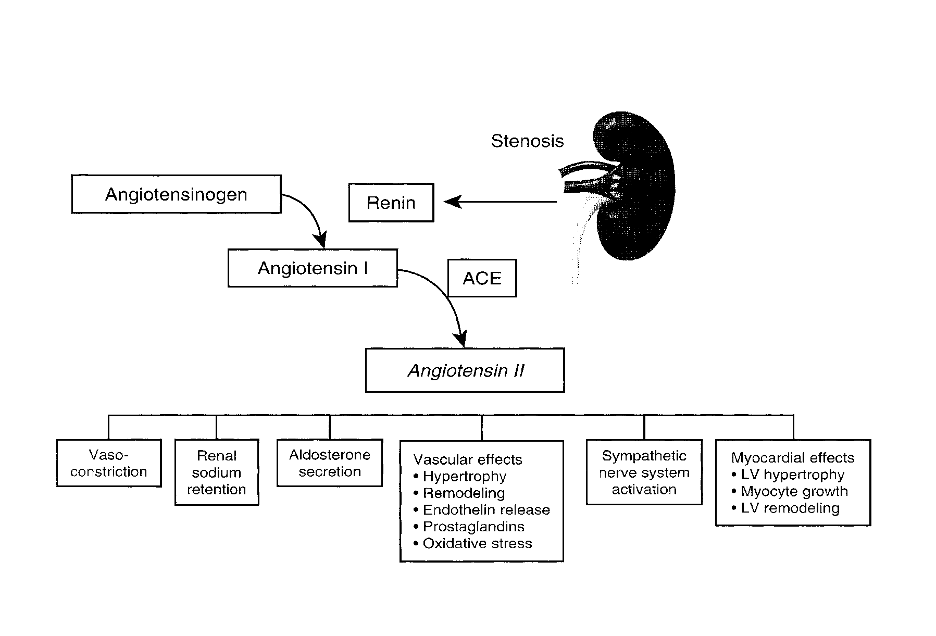
\includegraphics[width=13in]{images/renal1}

\textbf{I think the flow limitation part has been well established. What
next?}

Renal (especially bilateral) hypoperfusion induces activation of the
renin-angiotensin-aldosterone system which increases vascular tone and
impairs sodium excretion resulting in expansion of the extracellular
fluid volume.

\hypertarget{medical-management-and-evaluation}{%
\section{Medical Management and Evaluation}\label{medical-management-and-evaluation}}

\textbf{Can't we just treat their hypertension and give these patients an ACE
inhibitor at this point?}

Sure. And oftentimes we do. In fact, many of these patients can be
treated with medical therapy without loss of function or irreversible
fibrosis, sometimes for many years

\begin{itemize}
\item
  Studies in human subjects demonstrate that, despite a moderate
  reduction in renal perfusion pressure (up to 40 \%) and in renal
  blood flow (mean 30 \%), glomerular filtration is reduced but tissue
  oxygenation within the kidney cortex and medulla can adapt without
  the development of severe hypoxia.
\item
  But this only works to an extent.
\end{itemize}

\textbf{Explain that\ldots{}}

As the hypertension is treated, we're lowering the pressure gradient
across the stenosis and can actually increase the degree of renal
malperfusion and worsen the renal function.

\begin{itemize}
\tightlist
\item
  Oftentimes this loss of kidney function is a reversible consequence
  of antihypertensive therapy but it to some degree limits our ability
  to control the hypertension medically without causing further damage
  to the kidneys\ldots. And it can also reflect progressive narrowing of
  the renal arteries and/or progressive intrinsic kidney disease as
  more advanced vascular occlusion, corresponding to a 70 to 80\%
  narrowing of the renal artery, leads to demonstrable cortical
  hypoxia.
\end{itemize}

\textbf{Can we tell who has cortical hypoxia through diagnostic tests?}

A: To some degree. Cortical perfusion can be measured by blood oxygen
level dependent magnetic resonance (BOLD-MR). Additionally, inflammatory
markers sampled from renal veins of stenotic kidneys correlated strongly
with the degree of hypoxia (as measured by BOLD-MR), particularly after
correction of the stenosis with angioplasty

\textbf{So we have a patient with evidence of malperfused kidneys, either
through worsening renal function or uncontrolled hypertension, with
known discrete stenoses, and we even got a BOLD-MRI which confirms it.
Let's just revascularize them and be done with it?}

Not so fast. Although vascular stenosis or occlusion can initiate these
processes, long-standing ischemia causes parenchymal injury
characterized by inflammation and fibrosis which eventually becomes an
irreversible process. At some point, restoring renal blood flow provides
no recovery of kidney function or clinical benefit.

\textbf{So how can we determine who has CKD or hypertension due to
renovascular stenosis that we can actually help?}

This is probably the most important question since in this whole disease
process.

\begin{itemize}
\tightlist
\item
  To start, if a patient has the clinical manifestations of ischemic
  nephropathy or renovascular hypertension as we discussed above, a
  presumptive diagnosis of ischemic nephropathy can be made if there
  is radiologic documentation of significant stenosis (usually more
  than 70 \% luminal occlusion) of both renal arteries or of one renal
  artery to a solitary functioning kidney.
\end{itemize}

\textbf{But how do we know the vascular occlusive disease posing critical
hemodynamic limitation to kidney function?}

\begin{itemize}
\item
  Generally, luminal occlusion of at least 60 to 75 \% is required to
  limit blood flow and reduce perfusion pressure
\item
  This degree of stenosis is usually associated with a measurable
  translesional ``pull-back'' pressure gradient of 10 to 15 mmHg.
\item
  Doppler ultrasound criteria conventionally require peak systolic
  velocities above 180 to 200 cm/sec to identify more than 60 \%
  luminal stenoses but identifiable levels of cortical hypoxia
  (measured by blood oxygen level dependent magnetic resonance
  BOLD-MR) are usually associated with translesional velocities above
  385 cm/sec or reduction of single kidney glomerular filtration rate
  (GFR) in the range of 20 to 25 mL/min.
\end{itemize}

\textbf{Most importantly: is the condition of the kidneys such that restoring
renal blood flow is likely to benefit function?}

Short answer, we still can't be certain.

Long answer, we can at least have some idea by considering the renal
resistive index, the six-month trajectory of kidney function, and the
size of the kidneys or by performing a kidney biopsy (which is not
usually done).

\begin{itemize}
\item
  None of these factors predict the outcome of revascularization with
  certainty.
\item
  \underline{Improved and validated methods to evaluate the salvageability of
  kidney function in this disorder are greatly needed and are the holy
  grail of this disease process.}
\end{itemize}

\textbf{Let's go through some of these:}

\underline{Renal Resistive index:}

Some studies indicate that elevated resistive indices in segmental
vessels (above 0.80) measured by duplex ultrasound denote poor prognosis
for renal recovery while a low resistive index is a favorable sign.

\underline{Trajectory of kidney function}

The most consistent predictor of good recovery of kidney function after
revascularization has been a recent deterioration of kidney function
(ie, in the prior six to twelve months).

\underline{Kidney size}

Very small kidneys (less than 7 cm in longest diameter) are usually
considered unlikely to recover after revascularization.

\underline{Kidney biopsy}

Previous studies suggest that biopsy demonstrating preexisting
atheroembolic changes and interstitial fibrosis indicate a limited
potential for recovery.

\begin{itemize}
\tightlist
\item
  Biopsies are not usually performed.
\end{itemize}

\underline{Comparison of kidney morphology with kidney function}

Some investigators have recommended assessing morphologic parameters,
such as renal parenchymal volume and cortical thickness with MRI, and
comparing these parameters with kidney function measured by radionuclide
scanning

\begin{itemize}
\tightlist
\item
  In a stenotic kidney, apparently normal morphology combined with
  reduced function may indicate a ``hibernating kidney'' that could be
  salvaged with revascularization.
\end{itemize}

\textbf{So how do we get a definitive diagnosis?}

A definitive diagnosis is not usually made before revascularization. In
practice, confirmation of the diagnosis is based upon stabilization or
improvement of the GFR after successful revascularization.

\hypertarget{operative-managment}{%
\section{Operative Managment}\label{operative-managment}}

\textbf{Now we think our patient's renal artery stenosis maybe is causing
hypertension or decline in renal function and we can possibly reverse
it\ldots{} how do we treat it?}

For starters, all of these patients should receive medical therapy to
control their hypertension in addition to routine CKD care and
surveillance. They need to be aggressively treated for secondary
prevention of cardiovascular morbidity with aspirin, statins, cessation
of smoking, and, in patients with diabetes, glycemic control.

\textbf{Second, once diagnosis has been made we have 2 therapeutic
alternatives\ldots{} Which are?}

First, medical therapy alone- this generally involves ACE-I or ARB and
as we discussed.

Hemodynamically mediated acute kidney injury is the major limitation of
ACE inhibitors and ARBs in patients with bilateral renal artery stenosis
as lowering the systemic blood pressure is more likely to reduce the
renal perfusion and thus the intraglomerular pressure below the limits
of renal autoregulation\ldots{} in turn lowering the GFR.

\textbf{Okay, in other words we can have chronic normalization of the systemic
pressure that might eventually lead to ischemic atrophy due to the
reduced renal perfusion pressure distal to the stenosis? Any other
concerns with medical management alone?}

\begin{itemize}
\tightlist
\item
  We're addressing or prevention progression of stenosis in those with
  atherosclerotic disease.
\end{itemize}

\textbf{Since this isn't a vascular medicine podcast, what's our other
option?}

Procedural intervention (open or endovascular) along with medical
therapy.

\textbf{Now you're talking. Who should we fix operatively?}

Some but not all patients should undergo revascularization, Patient
selection single most important factor.

Depends upon the hemodynamic severity and likely recoverability of
kidney function

\textbf{You mentioned recoverability before, can you once again touch on what
helps us determine recoverability?}

\begin{itemize}
\item
  Recoverability indicators--

  \begin{itemize}
  \item
    A short duration of blood pressure elevation prior to the
    diagnosis of renovascular disease, since this is the strongest
    clinical predictor of a fall in blood pressure after renal
    revascularization
  \item
    Failure of optimal medical therapy to control the blood pressure
  \item
    Intolerance to optimal medical therapy (eg, deterioration of
    renal function during antihypertensive drug therapy)
  \item
    Recurrent flash pulmonary edema and/or refractory heart failure
  \item
    Otherwise unexplained progressive renal insufficiency,
    particularly if proteinuria is absent
  \end{itemize}
\end{itemize}

\textbf{But do we have any good data proving our interventions help?}

This is where things can get muddy.

Early on, observational studies demonstrated a high rate of procedural
success with percutaneous transluminal renal angioplasty (PTRA) and
stent placement (\textasciitilde85\%) in patients with ostial atherosclerotic disease,
as well as a high rate of clinical success measured by improvements in
blood pressure and kidney function in 50 to 75 \% of subjects.

\textbf{Anything better than observational studies?}

Unfortunately, randomized trials showed no additional benefit from
stenting when added to medical therapy with respect to blood pressure
control, renal function, cardiovascular events, and mortality. But these
studies have their own limitations.

\textbf{The one we keep hearing about is the CORAL trial. Tell me about
that.}

\begin{itemize}
\item
  CORAL trial \citep{cooperStentingMedicalTherapy2014}

  \begin{itemize}
  \item
    Cardiovascular Outcomes in Renal Atherosclerotic Lesions (CORAL)
    trial
  \item
    947 patients (80 \% had unilateral disease) who met the following
    two criteria:

    \begin{itemize}
    \item
      Unilateral or bilateral atherosclerotic renal artery
      stenosis \textgreater60 \% if diagnosed with conventional angiography,
      peak systolic velocity \textgreater300 cm/second if diagnosed by duplex
      Doppler ultrasonography, Luminal narrowing \textgreater80 \% if
      diagnosed with magnetic resonance angiography or
      computerized tomography angiography (or \textgreater70 \% with
      additional evidence of renal ischemia)
    \item
      Systolic hypertension despite two or more antihypertensive
      medications and/or an estimated glomerular filtration rate
      (eGFR) \textless60 mL/min/1.73 m2 that was presumably due to the
      stenosis.
    \item
      All patients received antiplatelet therapy plus best medical
      therapy including ARB
    \end{itemize}
  \item
    Revascularization had no additional effect on the primary
    outcome (a composite of cardiovascular or renal death, stroke,
    myocardial infarction, hospitalization for heart failure, a
    reduction in eGFR by more than 30 \%, or end-stage renal disease)
    as compared with medical therapy alone (35.1 versus 35.8 \%).
  \item
    No effect on any of the individual components of the primary
    outcome.
  \item
    Low procedural complication rate \textasciitilde2\%
  \end{itemize}
\end{itemize}

\textbf{Well, that sounds pretty convincing.}

\begin{itemize}
\item
  Limitations on existing treatment data:

  \begin{itemize}
  \item
    \underline{Considerable selection bias} -- For the most part, the
    patients enrolled in these trials did \textbf{not} meet the criteria
    for selecting patients likely to benefit from intervention (eg,
    short duration of blood pressure elevation, hypertension
    resistant to medical therapy, recurrent flash pulmonary edema):

    \begin{itemize}
    \item
      CORAL \citep{cooperStentingMedicalTherapy2014}

      \begin{itemize}
      \item
        Patients hospitalized for heart failure within 30 days
        of screening for the trial were excluded, thereby
        limiting the number of trial participants with recurrent
        flash pulmonary edema.
      \item
        Mean number of antihypertensive medications used by
        CORAL participants at baseline was 2.1- many had not
        failed optimal medical therapy
      \item
        More than 25 \% had controlled blood pressure upon entry
        into the trial.
      \item
        Mortality and event rates lower than in most previous
        registries, suggesting that many high-risk patients were
        not enrolled.
      \end{itemize}
    \item
      ASTRAL
      \citep{astralinvestigatorsRevascularizationMedicalTherapy2009}

      \begin{itemize}
      \tightlist
      \item
        Large number of patients had stenoses that were probably
        not clinically significant (50 to 70 \%), and patients
        were excluded if their primary doctors felt that they
        ``definitely'' needed revascularization.
      \end{itemize}
    \end{itemize}
  \item
    \underline{Results of the trials differ substantially from observational
    reports of ``high-risk'' subsets}

    \begin{itemize}
    \tightlist
    \item
      For the most part, patients selected by their treating
      clinicians to undergo revascularization have derived greater
      benefit from revascularization than did patients enrolled in
      the trials who were randomly assigned to revascularization
    \end{itemize}
  \end{itemize}
\end{itemize}

\hypertarget{endovascular-therapy}{%
\subsection{Endovascular Therapy}\label{endovascular-therapy}}

\textbf{We've determined our patient is an appropriate candidate for
intervention, and we don't fully buy into CORAL, what can we do?}

\begin{itemize}
\item
  \underline{Percutaneous renal angioplasty/stenting}in addition to medical
  therapy

  \begin{itemize}
  \item
    Most commonly employed if technically feasible.
  \item
    Most amenable lesions to angioplasty are those producing
    incomplete occlusion in the main renal artery.

    \begin{itemize}
    \tightlist
    \item
      Total occlusions and ostial lesions extending into aorta
      generally do not respond well to angioplasty alone due to
      elastic recoil.
    \end{itemize}
  \item
    Quick results: maximum antihypertensive response is generally
    observed at 48 hours after the procedure

    \begin{itemize}
    \tightlist
    \item
      But BP levels and antihypertensive drug requirements often
      change over subsequent weeks
    \end{itemize}
  \item
    In general, the effects of revascularization on blood pressure
    were greater in bilateral disease, but effects on renal function
    and mortality did not differ in those with bilateral as compared
    with unilateral stenosis .
  \item
    Most atherosclerotic lesions are now treated with primary
    stenting to avoid rapid development of restenosis.

    \begin{itemize}
    \item
      A higher initial primary success rate, defined as less than
      50 \% stenosis (88 versus 57 \%).
    \item
      At six months, a higher patency rate (75 versus 29 \%) and a
      lower restenosis rate (14 versus 48 \%).
    \item
      Twelve patients assigned to PTRA alone underwent stenting
      because of treatment failure within six months. These
      patients had a similar blood pressure response as those
      initially treated with stenting.
    \end{itemize}
  \end{itemize}
\end{itemize}

\textbf{What about complications?}

\begin{itemize}
\item
  Complication rate with percutaneous transluminal renal angioplasty
  with or without stenting is between 5 and 15 \%

  \begin{itemize}
  \item
    Mostly minor: puncture site hematoma and renal artery
    dissection.
  \item
    Serious complications more rare: renal artery thrombosis or
    perforation, AKI 2/2 atheroembolic disease (\textasciitilde1\%)or
    radiocontrast agent injury.
  \item
    Mortality exceedingly rare
  \end{itemize}
\end{itemize}

\textbf{Outcomes data}

\begin{itemize}
\item
  In the correct patient population:

  \begin{itemize}
  \item
    Unilateral disease

    \begin{itemize}
    \item
      PTRA alone results in normalization of blood pressure
      (removal of antihypertensive drug therapy) \textasciitilde8-20\%
    \item
      Some improvement 50-60\%
    \item
      Failure rate \textasciitilde20-30\%
    \item
      Restenosis rate of 8 to 30 \% at two years (without stent)
    \item
      Better results with unilateral fibromuscular disease.
    \item
      Less consistent for patients with chronic hypertension
      compared with patients who have an acute elevation in blood
      pressure
    \end{itemize}
  \item
    Bilateral disease

    \begin{itemize}
    \item
      25-30\% will recover kidney function to a meaningful degree,
      sometimes avoiding progression to end-stage kidney disease
      (ESKD) and/or the need for renal replacement therapy.
    \item
      \textasciitilde50\% will have little immediate change in kidney function
      but will ``stabilize''
    \item
      \textasciitilde20\% will have a progressive deterioration of kidney
      function, sometimes related to the procedure
    \end{itemize}
  \end{itemize}
\end{itemize}

\textbf{Guidelines}

\begin{itemize}
\item
  2005 ACC/AHA guidelines on peripheral artery disease recommends that
  a stent be placed in patients undergoing PTRA for treatment of
  atherosclerotic renal artery stenosis \citep{hirschACCAHA20052006}

  \begin{itemize}
  \item
    PTRA without stent placement is rarely performed unless the
    anatomy precludes stenting.
  \item
    POBA without stenting is generally less successful and
    associated with more complications (eg atheroemboli)
  \end{itemize}
\end{itemize}

\textbf{How durable is PTA/stenting?}

\begin{itemize}
\item
  Restenosis

  \begin{itemize}
  \item
    \textasciitilde11-17\%

    \begin{itemize}
    \tightlist
    \item
      11-39\% during the first one to two years
    \end{itemize}
  \item
    Detected as a rise in blood pressure requiring more intensive
    therapy
  \item
    Angioplasty/stenting injures the vascular endothelium, which may
    result in restenosis.
  \item
    Symptomatic stenosis leading to a rise in blood pressure or a
    fall in GFR are less common and are reported in 10 to 20 \% of
    patients
  \end{itemize}
\end{itemize}

\textbf{How do you follow these patients after stenting?}

\begin{itemize}
\item
  Follow-up of patients who have had a renal artery stent should
  include serial measurements of blood pressure and estimation of GFR.

  \begin{itemize}
  \item
    Post-stent duplex ultrasound @2-4weeks with
  \item
    Repeated examinations on a quarterly basis (not much data)
  \item
    Patients who develop an increase in pressure or reduced GFR
    after stenting should undergo duplex ultrasonography to identify
    restenosis
  \item
    Retreatment with angioplasty with or without repeat stenting can
    be attempted, but the restenosis rate after repeat angioplasty
    is increased.

    \begin{itemize}
    \tightlist
    \item
      Surgical reconstruction may be pursued in patients with
      recurrent episodes of restenosis and loss of kidney
      function.
    \end{itemize}
  \end{itemize}
\end{itemize}

\hypertarget{open-surgery}{%
\subsection{Open Surgery}\label{open-surgery}}

\textbf{What about an open operation?}

\begin{itemize}
\item
  \underline{Surgical revascularization} used in addition to medical
  therapy

  \begin{itemize}
  \tightlist
  \item
    Less common since the widespread application of effective
    antihypertensive drug therapy and endovascular stents (mid 90s)
  \end{itemize}
\end{itemize}

\textbf{So who still gets open repair?}

\begin{itemize}
\tightlist
\item
  Primarily for correction of complex vascular lesions and/or repeated
  episodes of in-stent restenosis
\end{itemize}

\textbf{How do we do it?}

\begin{itemize}
\item
  Involves bypassing the stenotic segment or of removing a small
  atrophic kidney with nearly complete arterial occlusion.

  \begin{itemize}
  \item
    From the aorta or hepatorenal or splenorenal bypass to avoid
    diseased aorta.
  \item
    Bilateral: either bilateral repair or unilateral repair with
    contralateral nephrectomy of a nonfunctioning, atrophic kidney.
  \end{itemize}
\end{itemize}

\textbf{How do outcomes compare to PTA/stenting?}

\begin{itemize}
\item
  Equally or more effective than PTRA in the treatment of
  atherosclerotic disease, with cure of or improvement in the
  hypertension occurring in 80 to 95 \% of patients.

  \begin{itemize}
  \tightlist
  \item
    Cure of hypertension after surgery is most likely in patients
    who have been hypertensive for less than five years
  \end{itemize}
\item
  Lack of complete response was usually associated with one of two
  factors:

  \begin{itemize}
  \item
    Presence of underlying primary/essential hypertension
  \item
    Development of intrarenal vascular disease due to exposure of
    the contralateral kidney to the elevated blood pressure.
  \end{itemize}
\end{itemize}

\textbf{Guidelines recommendations?}

\begin{itemize}
\item
  2005 American College of Cardiology/American Heart Association
  (ACC/AHA) guidelines \citep{hirschACCAHA20052006}

  \begin{itemize}
  \tightlist
  \item
    Open surgery in patients with atherosclerotic renal artery
    stenosis largely restricted to those who have multiple small
    renal arteries, have early primary branching of the main renal
    artery, require aortic reconstruction near the renal arteries
    for other indications (eg, aneurysm repair or severe aortoiliac
    occlusive disease), or to avoid manipulation of a highly
    diseased aorta or failed endovascular stents (using specific
    surgical techniques, including splenorenal, ileorenal, or
    hepatorenal bypass procedures).
  \end{itemize}
\end{itemize}

\textbf{So why not do it instead of stent?}

\begin{itemize}
\item
  In-hospital mortality: \textasciitilde3-10 \% in high volume centers

  \begin{itemize}
  \item
    Risk factors diffuse atherosclerosis, advanced age, chronic
    kidney disease, heart failure, or chronic lung disease.
  \item
    No deaths in 105 procedures for fibromuscular dysplasia (FMD).
  \end{itemize}
\end{itemize}

\hypertarget{fibromuscular-dysplasia-fmd}{%
\section{Fibromuscular Dysplasia (FMD)}\label{fibromuscular-dysplasia-fmd}}

\textbf{You mentioned FMD as a cause of renovascular hypertension, tell me
more about that\ldots{}}

Fibromuscular dysplasia (FMD) is a noninflammatory, nonatherosclerotic
disorder that leads to arterial stenosis, occlusion, aneurysm,
dissection, and arterial tortuosity.

\begin{itemize}
\tightlist
\item
  Virtually always diagnosed radiographically -- formerly
  pathologically, but rarely sent for specimen in modern diagnosis or
  treatment
\end{itemize}

\textbf{How do we classify it?}

\begin{itemize}
\item
  Most commonly classified by angiographic appearance:

  \begin{itemize}
  \item
    Multifocal FMD (more common)

    \begin{itemize}
    \item
      angiographic appearance of a ``string of beads.''
    \item
      corresponds pathologically to medial fibroplasia, the most
      common histologic type, and to perimedial fibroplasia, which
      is less common.
    \end{itemize}
  \item
    Focal FMD (less common)

    \begin{itemize}
    \item
      angiographic appearance of a ``circumferential or tubular
      stenosis''
    \item
      corresponds pathologically to intimal fibroplasia but medial
      hyperplasia and periarterial hyperplasia may also have a
      focal appearance.
    \end{itemize}
  \item
    These two different angiographic subtypes of FMD (multifocal and
    focal) have different phenotypic presentations and natural
    history

    \begin{itemize}
    \tightlist
    \item
      Is FMD is, in fact, a single disease?
    \end{itemize}
  \end{itemize}
\end{itemize}

\textbf{Where does it occur?}

\begin{itemize}
\item
  Has been observed in nearly every arterial bed
\item
  Involvement of the renal arteries \textasciitilde75-80\%
\item
  Involvement of the extracranial cerebrovascular arteries (eg,
  carotid and vertebral arteries) \textasciitilde75\%

  \begin{itemize}
  \tightlist
  \item
    2/3 of patients have multiple arteries involved.
  \end{itemize}
\end{itemize}

\textbf{Who has FMD?}

\begin{itemize}
\item
  \textasciitilde90\% of cases in adults are in women.

  \begin{itemize}
  \tightlist
  \item
    No female predominance among children with FMD.
  \end{itemize}
\item
  Mean age at diagnosis was 52 years, with a range of 5 to 86 years

  \begin{itemize}
  \tightlist
  \item
    In the past, it was believed that FMD was a disease of young
    women. However, older now know to make up a large proportion of
    affected
  \end{itemize}
\item
  35-50\% of cases in children and 5-10\% of cases in adults under the
  age of 60 years with renovascular hypertension
\item
  Often an incidental finding:

  \begin{itemize}
  \item
    4.4\% of potential kidney donors had evidence of FMD.
  \item
    CORAL trial:

    \begin{itemize}
    \tightlist
    \item
      FMD was discovered in 5.7\% of the total study population
      (8.8\% of enrolled females)
    \end{itemize}
  \end{itemize}
\end{itemize}

\textbf{What causes FMD?}

The etiology of FMD remains unknown, but some mechanisms have been
proposed

\begin{itemize}
\item
  Genetics may play an important role in development

  \begin{itemize}
  \item
    Some studies report autosomal mode of inheritance with variable
    penetrance
  \item
    Potential association with a single nucleotide variant in the
    phosphatase and actin regulator 1 gene (PHACTR1)
  \item
    Variant rs9349379 is also a risk locus for coronary artery
    disease, migraine headache, and cervical artery dissection.
  \end{itemize}
\item
  Predominance of young/childbearing age women hormonal influences are
  thought to play a role

  \begin{itemize}
  \tightlist
  \item
    Remains unproven.
  \end{itemize}
\item
  Mechanical factors such as stretch and trauma unproven.
\end{itemize}

\textbf{Does FMD present differently that the atherosclerotic renovascular
disease we talked about?}

\begin{itemize}
\item
  Varies widely depending on artery affected and as it results from:
\item
  Ischemia related to stenosis
\item
  Dissection and occlusion of major arteries (renal infarction,
  stroke, myocardial infarction)
\item
  Rupture of aneurysms
\item
  Embolization of intravascular thrombi from dissection or aneurysms
\end{itemize}

\textbf{What are the common presenting symptoms and signs}

\begin{itemize}
\item
  Manifestations of renal FMD (eg, hypertension, flank pain) are more
  likely to occur in men, as are arterial dissections and aneurysms.

  \begin{itemize}
  \item
    Most common presenting signs:
  \item
    Hypertension -- 67\% (66\% of women and 74 \% of men)
  \end{itemize}
\item
  But overall hypertension is the most common manifestation of renal
  artery FMD in both genders

  \begin{itemize}
  \tightlist
  \item
    Flank pain and abdominal pain can result from ischemia, aneurysm
    rupture, or dissection of renal and mesenteric arteries,
    respectively.
  \end{itemize}
\end{itemize}

\textbf{Are these dissections common?}

\begin{itemize}
\item
  High prevalence of aneurysm and/or dissection

  \begin{itemize}
  \item
    Aneurysm (22\%) and dissection (26\%).

    \begin{itemize}
    \item
      34\% of aneurysms were renal
    \item
      11\% of dissections were renal
    \end{itemize}
  \item
    42\% had an aneurysm and/or dissection.
  \end{itemize}
\end{itemize}

\textbf{So should we screen for these dissections in a patient with known
FMD?}

\begin{itemize}
\item
  Every patient diagnosed with FMD should have one-time,
  head-to-pelvic CTA (or MRA) is an alternative.

  \begin{itemize}
  \tightlist
  \item
    CTA of the neck and head on one day followed one week later by
    CTA of the chest, abdomen, and pelvis
  \end{itemize}
\end{itemize}

\textbf{When should we suspect FMD?}

\begin{itemize}
\item
  Hypertension (particularly in a woman under the age of 60 years)
  with findings that would prompt an evaluation for secondary
  hypertension:

  \begin{itemize}
  \item
    Severe or resistant hypertension.
  \item
    Onset of hypertension before the age of 35 years.
  \item
    A sudden rise in blood pressure over a previously stable
    baseline.
  \item
    A significant increase in the serum creatinine concentration
    after the institution of therapy with an angiotensin-converting
    enzyme (ACE) inhibitor or angiotensin receptor blocker (ARB) in
    the absence of an excessive reduction in blood pressure.
  \item
    An epigastric/abdominal bruit.
  \end{itemize}
\item
  Renal artery dissection (or carotid, vertebral, coronary)
\item
  Aneurysm in a visceral, carotid, vertebral, or intracranial vessel.
\item
  Renal infarction.
\end{itemize}

\textbf{How do we diagnose this and/or distinguish it from renovascular
atherosclerotic disease?}

\begin{itemize}
\item
  Confirmed by diagnostic imaging that reveals consistent findings
\item
  Noninvasive imaging test is usually performed first. This includes
  CTA, MRA, and Duplex ultrasound.
\end{itemize}

\textbf{Let talk about CTA\ldots{}}

\begin{itemize}
\item
  CTA is preferable due to higher spatial resolution than MRA, less
  dependence upon technical expertise, and a shorter scan time
\item
  Excellent diagnostic accuracy for FMD of the main renal arteries,
  although the sensitivity decreases when FMD is only present in the
  smaller branch renal arteries.
\item
  Multirow detector CT scanners, which offer more rapid image
  acquisition, variable section thickness, three-dimensional
  rendering, diminished helical artifacts, and smaller contrast
  requirements, may gain an increased role in the diagnosis and
  follow-up of renal artery FMD
\end{itemize}

\textbf{What about MRA?}

\begin{itemize}
\item
  Inconsistent detection of FMD and is performed if CTA is
  contraindicated
\item
  The spatial resolution in the branch vessels is not adequate, and
  artifact may occur, suggesting ``beading'' when none is present.
\item
  May miss mild FMD.
\item
  Can be useful for detecting aneurysms and dissections
\end{itemize}

\textbf{And finally, Duplex ultrasonography}

\begin{itemize}
\item
  Detects elevated blood flow velocities in the mid and distal
  portions of the renal artery, most common locations for FMD.
\item
  Increased peak systolic velocity, turbulent blood flow, and
  tortuosity of the mid and distal artery.

  \begin{itemize}
  \tightlist
  \item
    \% diameter stenosis reports less helpful and usually inaccurate
  \end{itemize}
\item
  lowest spatial resolution of all of the cross-sectional imaging
  modalities
\item
  most operator dependence
\item
  first choice only in high-volume centers with extensive expertise in
  this technique
\end{itemize}

\textbf{What about non invasive testing?}

\begin{itemize}
\item
  DSA is performed in patients if there is a high clinical suspicion
  of FMD, and treatment with revascularization is planned if a
  stenosis is found.

  \begin{itemize}
  \item
    Can improve visualization of the arteries by eliminating
    background soft tissue and bone and has higher spatial
    resolution than any of the other imaging modalities
  \item
    Can measure the pressure gradient across the stenosis

    \begin{itemize}
    \item
      Pressure decrease threshold of 10 \% or more of the mean
      pressure should be used to decide whether a lesion is
      hemodynamically significant
    \item
      IVUS and optical coherence tomography (OCT) can be helpful
      in determining if a dissection or intramural hematoma is
      present as well as help to determine if angioplasty has
      improved the stenosis.
    \end{itemize}
  \item
    Negative DSA excludes a diagnosis of FMD in the vascular bed
    that was imaged.
  \end{itemize}
\end{itemize}

\textbf{Any place for pathologic diagnosis in modern therapy?}

\begin{itemize}
\item
  Histopathology (and histologic classification) is \textbf{no longer} part
  of the diagnosis.

  \begin{itemize}
  \tightlist
  \item
    Only in the rare patient who requires surgical revascularization
    or resection of an aneurysm.
  \end{itemize}
\end{itemize}

\textbf{So how do we treat this, what warrants intervention and are those
interventions different than what we offer atherosclerotic disease of
the renal arteries?}

\begin{itemize}
\item
  All patients with FMD should be placed on antiplatelet therapy (ASA)
  unless otherwise contraindicated
\item
  \underline{Antihypertensive therapy}

  \begin{itemize}
  \item
    Most patients will require antihypertensive therapy, even if
    they undergo revascularization.
  \item
    Majority of patients with \textbf{focal} FMD have their blood
    pressure cured with angoplasty
  \end{itemize}
\end{itemize}

\textbf{But what about revascularization?}

\begin{itemize}
\item
  \underline{Revascularization} Goal: control of hypertension

  \begin{itemize}
  \item
    BP can be controlled in most adults with multifocal FMD with a
    mean of two antihypertensive medications
  \item
    Weigh risks and benefits in well controlled hypertension.
  \end{itemize}
\item
  \textbf{No} randomized trials comparing revascularization with medical
  therapy
\end{itemize}

\textbf{Well then who do we treat?}

\begin{itemize}
\item
  Recent-onset hypertension, with goal to cure hypertension.
\item
  Resistant hypertension despite compliance with an appropriate
  three-drug regimen.
\item
  Patients unable to tolerate antihypertensive medications or who are
  noncompliant with their medication regimen.
\item
  Adults with bilateral renal FMD, or unilateral renal FMD to a single
  functioning kidney, and unexplained progressive renal insufficiency
  thought to result from renal artery stenosis
\item
  Hypertensive children.
\item
  may be at higher risk than adults for progressive renal parenchymal
  loss, and therefore could benefit from revascularization even if
  their hypertension can be well-controlled with one or two
  antihypertensive medications.
\end{itemize}

\textbf{And what kind of results do we get with revascularization?}

\begin{itemize}
\item
  Hypertension is cured or improved following revascularization in a
  large proportion of patients with FMD.

  \begin{itemize}
  \item
    Much better than 2/2 atherosclerosis
  \item
    Varies considerably from study to study, although hypertension
    control improves in most patients and depends in large part upon
    the definition of cure.
  \item
    Not good data on stabilization of either GFR or renal size in
    patients with FMD.
  \end{itemize}
\end{itemize}

What options do we have in terms of revascularization?

\textbf{Angioplasty and open surgery}

Do we have good results treating FMD with these?

\begin{itemize}
\item
  Improvement in blood pressure (including those with and without
  cure) was similar with PTA as compared with surgery (86 versus 88
  \%).
\item
  Older age and longer duration of hypertension prior to
  revascularization were significantly associated with a lower cure
  rate.
\end{itemize}

\textbf{How do these compare?}

\begin{itemize}
\item
  PTA achieves similar technical success and is associated with a
  lower risk of adverse events in observational studies
\item
  Most patients with FMD who are selected for renal revascularization
  have PTA rather than surgery
\item
  Major adverse events were more frequent with surgery (15 versus 6
  \%).
\end{itemize}

\textbf{So why choose open surgery?}

\begin{itemize}
\item
  Cure rates were higher with surgery (54 versus 36 \%).
\item
  Surgery rather than PTA if PTA fails or if the arterial anatomy is
  not amenable to PTA

  \begin{itemize}
  \tightlist
  \item
    Patients with small renal arteries (\textless4 mm), with branch renal
    artery disease, or with extensive intimal fibroplasia.
  \end{itemize}
\end{itemize}

\textbf{So how do we perform Percutaneous transluminal angioplasty} for FMD?

\begin{itemize}
\tightlist
\item
  \underline{Without} stent placement\ldots{} unlike PTA for atherosclerotic RAS
\end{itemize}

\textbf{Why not place a stent?}

\begin{itemize}
\item
  Patients do very well with angioplasty alone, no reason to place a
  stent.

  \begin{itemize}
  \item
    Lesion is so fibrotic that the pressure gradient cannot be
    obliterated with an angioplasty, a stent will not correct this
    problem

    \begin{itemize}
    \tightlist
    \item
      Such patients should be referred for surgery.
    \end{itemize}
  \end{itemize}
\item
  Usually have stenoses in the mid and distal portions of the artery
  rather than at the ostium or proximal portion (as occurs with
  atherosclerosis).

  \begin{itemize}
  \tightlist
  \item
    Should surgical revascularization become necessary due, for
    example, to in-stent restenosis, patients may require more
    complex branch repair to bypass the occluded stent since the
    stent often covers the renal artery up to the point of the first
    intrarenal branch.
  \end{itemize}
\end{itemize}

\textbf{Do we ever place stents?}

\begin{itemize}
\tightlist
\item
  Stents placed when a dissection results from the performance of PTA
  or in the rare instance in which a perforation of the renal artery
  occurs during angioplasty.
\end{itemize}

\textbf{And we're getting good outcomes with PTA alone?}

\begin{itemize}
\item
  Technical (angiographic) success rates for PTA 83-100
\item
  Rate of restenosis 12-34\% over follow-up intervals of six months to
  two years

  \begin{itemize}
  \item
    Difficult to determine if patients with FMD develop restenosis,
    or if the lesion was not completely treated correctly the first
    time.
  \item
    Not necessarily associated with recurrent hypertension.
  \end{itemize}
\end{itemize}

\textbf{But generally we can achieve significant and sustained reductions in
systolic blood pressure, diastolic blood pressure, serum creatinine, and
number of antihypertensive agents.}

\begin{itemize}
\tightlist
\item
  Systolic blood pressure response was better in patients with FMD
  affecting the main renal artery than in patients with branch vessel
  involvement.
\end{itemize}

\textbf{Any specific technical tips?}

\begin{itemize}
\item
  Cutting balloon angioplasty should be avoided

  \begin{itemize}
  \tightlist
  \item
    Increased risk of rupture
  \end{itemize}
\item
  Post angioplasty visual inspection alone is \textbf{not} accurate.

  \begin{itemize}
  \item
    Measure pressure differential using a pressure guidewire, with a
    mean gradient of \textless5 mmHg across the treated segment suggesting
    a satisfactory result

    \begin{itemize}
    \tightlist
    \item
      Measure before and after angioplasty
    \end{itemize}
  \item
    Post-procedure renal duplex scanning

    \begin{itemize}
    \tightlist
    \item
      Degree of turbulence is less prominent, and velocity
      elevation in the mid-distal renal artery returns to normal.
    \end{itemize}
  \item
    Intravascular ultrasound or optical coherence tomography (OCT)
    is occasionally used to evaluate the elimination or reduction of
    various endoluminal defects.
  \end{itemize}
\end{itemize}

\textbf{What should we do if it doesn't work?}

\begin{itemize}
\item
  If either has no improvement in blood pressure or an initial
  improvement followed by recurrence, repeat angiogram and PTA.

  \begin{itemize}
  \tightlist
  \item
    Restenosis may actually represent inadequate angioplasty during
    the first procedure
  \end{itemize}
\item
  Persistent HTN despite technically successful PTA suggests that the
  cause of hypertension is unrelated to fibromuscular disease or is
  related to small vessel disease within the kidney (nephrosclerosis)
  due to longstanding hypertension.
\end{itemize}

\textbf{What kind of complications do we see after this?}

\begin{itemize}
\item
  Mostly related to vascular access
\item
  Rarely: renal artery perforation, dissection, or segmental renal
  infarction may occur.
\item
  Decreasing over time- 16 \% in 1998 to 3 \% in 2001
\end{itemize}

\textbf{Ok, lets switch gears to open revascularization?}

\begin{itemize}
\item
  Aortorenal bypass with a saphenous vein graft is the most common
  technique

  \begin{itemize}
  \tightlist
  \item
    Artificial graft material used occasionally
  \end{itemize}
\end{itemize}

\textbf{For everyone? What about for pediatric patients?}

\begin{itemize}
\tightlist
\item
  Pediatric patients: hypogastric artery grafts are used or else
  aortic reimplantation of the renal artery is performed because vein
  grafts become aneurysmal
\end{itemize}

\textbf{How does this compare again to PTA?}

\begin{itemize}
\item
  Similar success rates compared to PTA (82-89\% patency) but with
  higher morbidity.

  \begin{itemize}
  \item
    Perioperative mortality appears to be very low (\textasciitilde1.2\%)
  \item
    Usually limited to complex cases so success and complication
    would probably be higher if simpler cases were included.
  \end{itemize}
\end{itemize}

\textbf{What's Monitoring and follow-up look like for these patients?}

\begin{itemize}
\item
  Medical management only:

  \begin{itemize}
  \item
    Renal artery stenosis and kidney dysfunction may progress
    despite good blood pressure control

    \begin{itemize}
    \tightlist
    \item
      Mostly in patients with focal FMD and intimal fibroplasia
    \end{itemize}
  \item
    Every patient with FMD should have measurement of serum
    creatinine and renal artery duplex ultrasound every 12 months.
  \end{itemize}
\end{itemize}

\textbf{And After revascularization}?

\begin{itemize}
\item
  Duplex ultrasonography and serum creatinine measurements performed
  on the first office visit post procedure, then every six months for
  two years, and then yearly, if stable.
\item
  With worsening on new hypertension, or unexplained increase in the
  serum creatinine, he or she should be imaged at that time with
  duplex ultrasound (or CTA if the ultrasound is equivocal or poor
  quality).
\end{itemize}

\hypertarget{renal-artery-aneurysms}{%
\section{Renal Artery Aneurysms}\label{renal-artery-aneurysms}}

\textbf{Ok, that's a pretty good review, but let's switch gears and talk about
renal artery aneurysms}

\begin{itemize}
\item
  Renal artery aneurysms are rare.

  \begin{itemize}
  \item
    Autopsy studies have revealed an incidence of 0.01\% to 0.09\%.
  \item
    Renal artery aneurysms are bilateral in about 10\% of cases with
    more than 90\% of true renal artery aneurysms being
    extraparenchymal.
  \end{itemize}
\item
  Females \textgreater{} males

  \begin{itemize}
  \tightlist
  \item
    Females and males equal with FMD excluded
  \end{itemize}
\item
  Most frequent site of involvement is primary bifurcation,
  intraparenchymal (\textless10\%)
\item
  Most are saccular
\item
  Right slightly more common than left, bilateral 10\%
\item
  Size criteria currently controversial*

  \begin{itemize}
  \item
    2.5 common criteria for visceral arterial intervention, but
    paucity of data suggesting rupture risk drastically increases at
    this size
  \item
    Many aneurysms with circumferential calcification which could
    offer protection against rupture
  \end{itemize}
\item
  The majority of renal artery aneurysms are asymptomatic, and less
  than 3\% rupture.

  \begin{itemize}
  \item
    Present with flank pain, hypotension
  \item
    10\% mortality
  \item
    90\% risk of kidney loss
  \end{itemize}
\item
  Although arteriosclerotic changes have been identified in most
  aneurysms in patients with multiple lesions, this is not a uniform
  finding, suggesting that arteriosclerosis may not be the most
  important factor in the genesis of renal artery aneurysms.
\item
  More likely due to a congenital medial degenerative process with
  weakness of the elastic lamina.
\item
  Fibromuscular dysplasia (FMD) is often a direct contributor to the
  development of an aneurysm.

  \begin{itemize}
  \item
    Medial fibroplasia is typically associated with multiple
    stenoses and post-stenotic dilatation of the distal two thirds
    of the renal artery.
  \item
    Renal artery aneurysms in association with FMD are generally
    only a few millimeters in diameter.
  \item
    The typical angiographic appearance of a renal artery involved
    with medial fibroplasia is a ``string of beads.''
  \end{itemize}
\item
  The majority of renal artery aneurysms are saccular.
\item
  A rare cause of renal artery aneurysms is Ehlers-Danlos' syndrome.

  \begin{itemize}
  \tightlist
  \item
    This disorder is associated with extreme arterial fragility and
    spontaneous rupture.
  \end{itemize}
\item
  Renal artery dissection caused by guide wires or catheters can
  occur, but is rare.
\item
  In an elderly patient, observation of this aneurysm with Duplex
  surveillance is the appropriate treatment.
\item
  For larger aneurysms in younger patients, aneurysmorrhaphy with
  primary repair or patching can be performed with low mortality.

  \begin{itemize}
  \tightlist
  \item
    Endovascular techniques such as coiling have been reported to be
    successful in treating these saccular aneurysms; however,
    covered stent placement may be difficult in the distal renal
    artery near potential branch points of the artery.
  \end{itemize}
\end{itemize}

\hypertarget{thoracic-aorta}{%
\chapter{Thoracic Aorta}\label{thoracic-aorta}}

\hypertarget{aortic-dissection}{%
\section{Aortic Dissection}\label{aortic-dissection}}

\textbf{01 Nov 2021:} \emph{Matt Spreadbury, MD; Adham Elmously, MD; Einar Brevik,
MD and Joseph Lombardi, MD}

\textbf{What~is an aortic dissection?}

It's when a tear occurs in the intima that results in separation of
layers of the intima and media and allows blood to flow through the
false lumen.

\textbf{How common are they and how serious are they?}

Acute dissections occur around 3/100000 - 2-3x more common than ruptured
aortic aneurysm. For Type A dissections, early mortality 1-2\% per hour -
if untreated,~20\% die within 6 hours, 50\% within 24 hours, 70\% first
week.~

Main cause of death in type A is aortic rupture into the pericardium,
acute aortic regurgitation, and coronary ostia compromise. While
patients with descending thoracic aortic dissections are more likely to
die from end organ compromise due to obstruction of visceral or
extremity vessels in the acute phase of the disease.~

\textbf{The time frame is also important.}

\begin{itemize}
\item
  Hyperacute \textless24 hours~
\item
  Acute~ \textless{} 2 weeks ~
\item
  Subacute 2 weeks -- 3 months -\textgreater{} TEVAR
\item
  Chronic \textgreater3 months~ -\textgreater{} Chronic aneurysmal degeneration/ partial false
  lumen thrombosis (highest risk) = operative treatment
\end{itemize}

\textbf{When we think about aortic dissections there are a few
classifications, how can we break it down?}

Historically, there are the Stanford and Debakey Criteria.

Anatomical Stanford

\begin{itemize}
\item
  ~Type~ A - involves the ascending aorta, 2/3 (most common)
\item
  ~Type~ B - arises from distal to L subclavian, 1/3
\end{itemize}

Debakey

\begin{itemize}
\item
  A

  \begin{itemize}
  \item
    1 - ascending + descending
  \item
    2 - ascending only
  \end{itemize}
\item
  B - distal or at the LSCA.

  \begin{itemize}
  \item
    3a - Descending aorta above diaphragm
  \item
    3b - Descending aorta above and below diaphragm
  \end{itemize}
\end{itemize}

\textbf{How about the new system proposed by Dr Lombardi, the SVS-STS
classification system?}

The new system published in 2020 keeps A and B and adds a number system
which divides the aorta into zones from 0 proximaly to 12 distally in
the mid SFA. \citep{lombardiSocietyVascularSurgery2020}

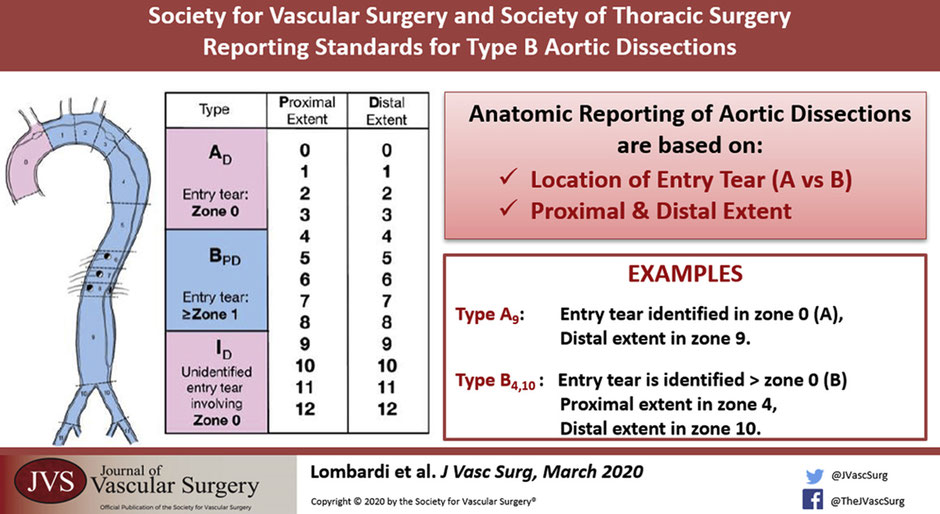
\includegraphics[width=13.06in]{images/thoracic_dissection1}

\begin{itemize}
\item
  Type A is now JUST the ascending aorta to the innominate, also
  called Zone 0.~
\item
  Type B is now~an entry tear in Zone 1 or greater~and distally to
  whichever zone the dissection lands in.
\end{itemize}

\textbf{This anatomical}~\textbf{classification~is based on reading the CT angio.
What else could we see on a CT angio that we have to know about?}

So aside from the aortic dissection its self, you could see a bleb of
contrast sticking out. That could be an penetrating aortic ulcer. That
is an atherosclerotic lesion that penetrates the internal elastic lamina
of the aortic wall.

Another key finding can be an intramural hematoma which is a hyperdense
crescent shaped hemorrhage within the aortic wall. There is no
identifiable direct communication between the true and false lumen. IMH
are classified in the same way but with the abbreviation IMH p-d zones.

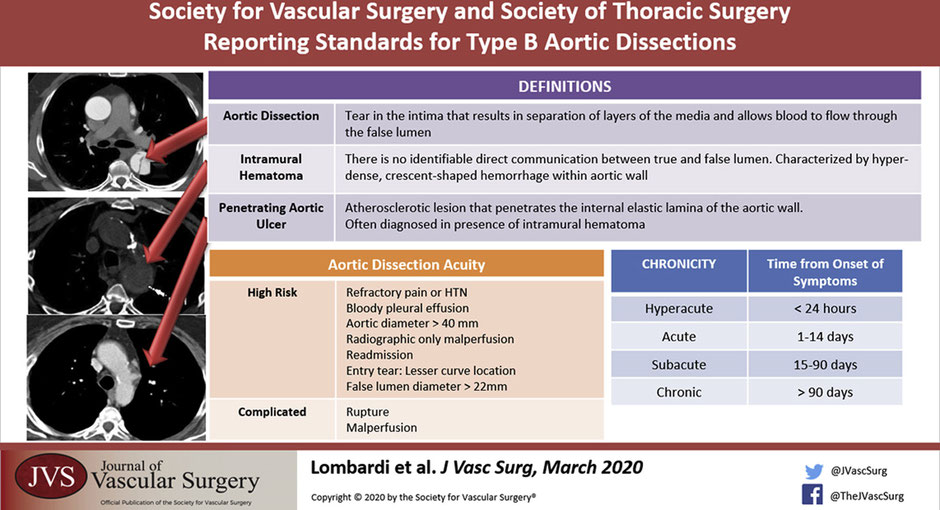
\includegraphics[width=13.06in]{images/thoracic_dissection2}

\textbf{Whats the significance of these two in combination?}

There is a higher chance of aortic rupture if a penetrating aortic ulcer
is seen with intramural hematoma.

\textbf{When a patient presents with an aortic dissection how can we classify
them clinically?}

\begin{itemize}
\item
  Uncomplicated~

  \begin{itemize}
  \item
    Stable hemodynamics~
  \item
    No evidence of malperfusion
  \item
    Pain controlled~
  \end{itemize}
\item
  Complicated~

  \begin{itemize}
  \item
    End organ ischemia / malperfusjon
  \item
    Rupture or impending rupture
  \end{itemize}
\item
  High risk~

  \begin{itemize}
  \item
    Uncontrollable pain / hypertension~
  \item
    Bloody pleural effusion
  \item
    Aortic diameter \textgreater40mm / False lumen diameter \textgreater{} 22mm
  \item
    Readmission
  \item
    Radiographic only malperfusion~
  \item
    Entry tear on the lesser curve
  \end{itemize}
\end{itemize}

\textbf{What is the danger of a false lumen? How does it lead to symptoms and
malperfusion? Likewise which arteries commonly branch off the true
lumen?}

The false lumen can lead to end organ ischemia as the intimal flap can
cover the ostia of branching vessels. This can be a static or a dynamic
obstruction.

Likewise it also leads to weakening in the wall of the aorta which can
become a threatened rupture or rupture if the diameter of the false
lumen is larger than 22mm.~

The celiac trunk, SMA, right renal typicaly come of the true lumen. Left
renal comes off the false.~

Also the dissection most commonly goes down into the left common illiac
rather than the right. You might be able to detect down stream effects
of this on clinical exam with reduced left sided groin pulse.

\textbf{What kind of patients get aortic dissections?}

Hypertension (older patients) / cocaine or Meth (younger patients)~

Marfans, loeys-Dietz, Ehlers danlos Type 4, Turners, Arteritis, Bicuspid
aortic valve.

We also have a traumatic cause of aortic dissections. That being called
blunt thoracic aortic injury:

\begin{itemize}
\item
  Grade 1: intima tear
\item
  Grade 2: IMH
\item
  Grade 3: Pseudo aneurysm
\item
  Grade 4: Aortic rupture.
\end{itemize}

\textbf{How do these patients present?}

Signs and symptoms --~Chest pain 90\% tearing pain radiating between the
shoulder blades.~

Chest pain extending to the abdomen abdomen? Think mesenteric ischemia
or aortic tear

Type A - Stroke 5-10\%,~Syncope 15\%, tamponade, carotid dissection,
paralysis.~

Others: MI -- Hypovolemic shock -- leg ischemia

\textbf{What is the~workup?}

Physical Exam --~Asymmetric pulses / blood pressure differences /
Diastolic murmur,

Investigations - CXR, EKG, D-dimer + Troponin, CTA, ECHO for type A.~

The big distinction is to find out if this is a type A or type B because
the treatment strategy is completely different.

\begin{itemize}
\item
  Type A need an emergent operation
\item
  Type B starts with medical management, follow up~CT angio~ +/- Trans
  esophageal echo in the OR. Reevaluate at 24 hours.~
\end{itemize}

\textbf{What are the details of Type A treatment?}

Operative treatment. 30\% op mortality. Cardiothoracics take the lead on
this one. However vascular surgeons should be involved in the management
of type A as after the repair, a type A can become a functional type B.

Type B is in the realm of vascular surgery. What is the first management
step after we have diagnosed a type B dissection?

Invasive impulse therapy. That means redusing the force of transmitted
impulse down the aorta. Blood pressure goals of 100-120mmHg. Hr \textless{}
60bpm.~

\textbf{How would you achieve that?}~

Start with a beta-blocker (esmolol or labetalol) first then a
vasodilator (nitroprusside). This is to stop the sympathetic surge after
vasodialation that could increase pressure and thus tearing forces
inside the aorta worsening the dissection.~

Initial CT, 72 hours, 3 months x 4, q6 months x2, q12 month. (Descending
thoracic aorta that dialates first.)~

\textbf{Why isnt open surgery indicated for type B dissections?}

Open surgery is not recommended due to the high mortality 30\% if \textless{} 48
hours. 18\% if \textgreater{} 49 hours.~

In the acute setting mortality can be up to 50\% with a 20\% paraplegia
risk. Its been described as sowing tissue paper.

\textbf{What is the management plan for a complicated Type B aortic
dissection?}

Start with invasive medical management and plan for TEVAR.~The goal with
TEVAR being to direct the blood flow into the true lumen and seal the
entry tear.~ If there was a dynamic obstruction (flap occludes branching
vessels.) Then TEVAR would reestablish the true lumen hence removing the
dynamic obstruction. Endovascular fenestration can also equalise the
pressure in the true and false lumen. \citep{lombardiSTABLEIIClinical2020}

For a static occlusion there could be a thrombus or stenosis in the
branched vessel so a stent might be indicated.~

\textbf{What are the major risks of TEVAR in the management of Type B aortic
dissections?}

Retrograde type A (reported 2\% in literature however it can be around
20\% in some experiences), 5\% paraplegia, and stent induced new entry.

\textbf{Is there a role for TEVAR in uncomplicated type B dissections?}

The INSTEAD and INSTEAD XL trials looked at uncomplicated Type B
dissections. There was NO statistical difference at 2 years comparing
OMT vs TEVAR but at 5 years there was good aortic remodelling and better
long term survival in patients treated in the subacute stage.~

Timing for TEVAR is a difficult choice. In chronic dissections the
septum thickens leading to a potentially difficult TEVAR. ~Anecdotally
TEVAR is best at 2w-3m.

\hypertarget{thoracoabdominal-aneurysms-taaa}{%
\section{Thoracoabdominal Aneurysms (TAAA)}\label{thoracoabdominal-aneurysms-taaa}}

02 Dec 2021: Mr.~Mohamed Barkat, Mr.~Nick Greaves, and Mr.~Michael
Jenkins

Resources

\begin{itemize}
\item
  \href{https://pubmed.ncbi.nlm.nih.gov/3951025/}{Crawford
  Classification}
\item
  \href{https://www.esvs.org/wp-content/uploads/2015/12/Consensus-document-ESVS-EATCS-Aortic-Arch.pdf}{ESVS recommendation of management of Thoracic aortic
  pathologies}
\item
  \href{https://www.optechtcs.com/article/S1522-2942(18)30073-4/fulltext}{Open Repair of Thoracoabdominal Aortic Aneurysm:
  Step-by-Step}
\item
  \href{https://www.circulationfoundation.org.uk/}{\textless https://www.circulationfoundation.org.uk\textgreater{}}
\item
  \href{https://www.bset.co.uk/}{\textless https://www.bset.co.uk/\textgreater{}}
\item
  \href{https://www.vascularsociety.org.uk/}{\textless https://www.vascularsociety.org.uk/\textgreater{}}
\item
  \href{https://podcasts.apple.com/us/podcast/yale-vascular-review/id1587352652}{Yale Vascular Review Podcast Episode 1: Thoracoabdominal
  Aneurysms}
\end{itemize}

\hypertarget{aortopathies}{%
\section{Aortopathies}\label{aortopathies}}

\textbf{18 May 2020}: \emph{Dr.~Anna Ohlsson and Dr Sherene Shalhub; University of
Washington}

\textbf{What are the common genetic aortopathies?}

There are several well-known genetic disorders which account for genetic
aortopathies. The most well-known are Marfan syndrome, Loeys-Dietz
Syndrome, and Vascular Ehlers-Danlos Syndrome,

There are less commonly known ones such as Familial Thoracic Aortic
Aneurysms and Dissections due to pathogenic variants smooth muscle cells
genes such as~\emph{ACTA2}. There are others in which the causative gene is
not known.

\textbf{Why are they such a big deal?}

These are cases in which the building blocks of the aortic wall are
defective. What~ I mean by this, is that these patients have pathogenic
variants in the genes that affect cell signaling or smooth muscle cell
structure that lead to suboptimal composition of the aortic wall.~ These
alterations ultimately lead to cystic medial necrosis in the aortic
wall.

As such they are at more risk for aortic aneurysms and dissections that
can lead to the premature death of the patient.

To put the frequency in perspective, Marfan syndrome occurs in 1:5000 of
the population while Vascular Ehlers-Danlos syndrome (also known as
VEDS) occur in 1:50000 of the population.

\textbf{Let's dive into them then -- what are the defining features of each
and the high yield information?}

The high yield information is being able to pair the genetic syndrome
and phenotype with its associated genetic mutation.~ A useful exercise
following this broadcast is to list the disorders in a table and write
out their associated gene mutation, what protein defect or deficit
occurs, the typical phenotype, and the common vascular pathology
associated.

But before we dive in, I want you to keep in mind some of shared
features.~ One is that the associated aneurysms and dissections tend to
occur at younger ages and dissect at lower blood pressures than what we
see with sporadic dissections (these are the dissections that are not
familial or associated with a syndrome)

One is that these are inherited in an autosomal dominant matter but
there can be variation in how the pathogenic variants are expressed
among affected people and even within families. The other thing to
remember, is that in roughly half of these cases, the affected patient
is the first in their family to have a given pathogenic mutation. The
flip side of this, is in half the cases, there is a family history of
aortic aneurysms, dissections, and sudden death.

\textbf{We will start with Marfan syndrome.}

\underline{Marfan syndrome} is caused by pathogenic variants in
the~\emph{FBN1}~gene (also known as fibrillin-1 gene). These variants lead to
improper formation of the microfibrils that maintain elastin, a key
component of the arterial wall.~

These patients are prone to aneurysmal degeneration and dissections of
the aortic root but can also dissect the descending thoracic aorta. They
commonly have lens dislocations (ectopia lentis).~ They have common
skeletal features such as

being tall, thin,~with long arms and legs, scoliosis, pectus deformities
(carnitatum or exicavtum), and club feet. They can also have a history
of spontaneous pneumothoraces and mitral valve prolapse.

\textbf{How is Marfan syndrome similar or different from the other genetically
triggered aortopathies that you mentioned?}

\underline{Loeys Dietz Syndrome} is similar to Marfan syndrome in all the
features including the aortic root aneurysms. They don't seem to have
lens dislocation and they have other unique features such as bifid uvula
or cleft palate, and hypertelorism (which is an abnormally increased
distance between the eyes). ~What is different about Loeys Dietz
Syndrome from Marfan syndrome is that they can have arterial aneurysms
of other arteries instead of the aorta, such as the SMA, axillary, or
other peripheral arteries.

\underline{Vascular Ehlers-Danlos syndrome} has some shared features to
Marfan Syndrome with both such as spontaneous pneumothoraces, but these
patients tend to be short and can have easy bruising. They also have
similar features to Loeys Dietz syndrome in terms of arterial aneurysms.
Common features of VEDS would be thin translucent skin where you can
easily see their veins, thin lips, thin bridge of the nose, large eyes,
easy bruising, acrogeria -- or an aged appearance of the hands

However, unlike Marfan and Loey Dietz, the majority of VEDS patients
tend to not have aortic root aneurysms. One thing to remember about VEDS
is that it is a~\emph{subtype}~of Ehlers Danlos syndromes.~ It's very
important to distinguish it from the other subtypes because most of the
other 12 Ehlers-Danlos syndromes are not associated with arterial
pathology. So people with vascular EDS are prone to arterial, uterine,
and intestinal rupture and their average lifespan is 48 due to these
highly morbid pathologies.~ 25\% of patients with vEDS will have
experienced some clinical manifestation by age 20, and that number is
close to 90\% by age 40.~~~

\textbf{I remember learning about classic Ehler's Danlos presenting with
hypermobile skin and joints.~ Is this something you see with Vascular
EDS as well?}

Patient's with vEDS don't have the same hypermobile skin or joint laxity
as we classically think of with classic Ehler's Danlos.~ In fact, some
vEDS patients report losing confidence in their physicians who ask them
about joint and skin hypermobility because it suggests to them that
their doctor doesn't know about their disease process.~ These patients
often know more than most of the doctors they meet about their
condition, and it's a source of constant frustration for them.~ It can
also be a problem if the severity of the disease is underestimated, as
we discussed they can present much younger than most patients with
highly morbid issues -- like arterial rupture.

\textbf{You mentioned arterial pathology in Loeys Dietz and VEDS. Can you tell
me more about that?}

In both types you can see subclavian, carotid, SMA, and iliac artery
aneurysms and dissections, as well as less frequently vertebral, SFA,
and popliteal aneurysms and dissections.

\textbf{How do you diagnose these genetically triggered aortopathies?}

There are clinical diagnostic criteria for each, but ultimately genetic
and laboratory testing is very important for the final diagnosis.

Ghent's criteria is used to clinically diagnose Marfan's syndrome. The
big ones are aortic root dilation, known family history of Marfan's or
not, the diagnosis of ectopia lentis which clinically is manifested as
iridonesis (lens shimmering). Additionally, genetic testing for
pathogenic FBN1 variants is also diagnostic.

To date, there are 5 types of Loeys-Dietz as of last check. These are
due to pathogenic variants in the TGF-B signaling pathway, such as
TGF-beta receptors and SMAD3 genes.~

Vascular EDS is caused by a mutation in the COL3A1 gene which encodes a
defective type of III procollagen.~ The defect in the procollagen makes
it unable to properly fold into a triple helix that forms the normal
collagen structure.~ This causes the defective procollagen to be
degraded intracellularly and as a result there is an overall deficit in
type III collagen which is an important component of arterial walls and
other structures.~ The confirmatory test for VEDS is collagen testing
which can confirm the collagen III defect.

\textbf{How would you manage these patients?}

Medical optimization and surveillance is key to try to extend the time
as much as possible before they get a dissection and avoid it if at all
possible.~

We start with lifestyle modification.~ Avoid ``burst'' exertions such as
sprinting and weight-lifting.~ Anything that very strenuous.~~ That's
not to say that they shouldn't exercise.~ Light exercise is encouraged,
but this would be activities like light jogging, swimming laps, or
biking.~

In order to minimize aortic shear stress, a resting heart rate of under
70 beats per minute and an exercising heart rate under 100 should be the
goal.~ This can be accomplished with beta blockers.~ Propranolol has
been shown to significantly decrease the rate of aortic growth in
Marfans patients with a baseline aortic root diameter under 4cm.~ There
is research into the use of Losartan in murine models that suggests it
inhibits TGF-beta in the aortic wall, which is an important pathway that
contributes to the breakdown of the wall. ~However, randomized
controlled studies have failed to show an increased benefit of Losartan
over beta blockers in Marfans patients. ~ACE inhibitors are also being
tested and are shown to decrease the risk of type b aortic dissection
over 6 years.

In vascular EDS instead of propranolol, celiprolol has been studied by
the French and shown to reduce vascular rupture from 50 down to 20\% in
vEDS, although the mechanism of this is not yet clear and does not
appear to be necessarily the same as decreasing shear stress as in
Marfan's syndrome.~~ In general taking care of these patients involves
trying to minimize complications from procedures and interventions.~ For
instance, use ultrasound for any line that is necessary and avoid
arterial lines, intramuscular injections, or other invasive lines if
possible to minimize the chance of a complication.~ Patients are advised
to wear medical bracelets notifying that they have vEDS.

We also discuss the importance of forming a care team based on their
needs. This usually includes a cardiologist, a cardiac surgeon, a
vascular surgeon, and a primary care physician.

\textbf{What about surgical treatment for those who need it?}

For patients with Marfan's, prophylactic surgery is recommended for
aortic root dilation \textgreater5cm or thoracic aorta \textgreater5.5cm.~ Often times the
thoracic and abdominal aorta are involved.~ Open and endovascular
surgery are options for these patients. Open procedures often include
open thoracoabdominal aortic aneurysm repairs, open cardiac surgery for
arch replacement, or cervical debranching procedures.~ Endovascular
procedures can include regular TEVARs or branched TEVARs which require
extensive aortic coverage.~ Open surgery can be well tolerated and is
ideal in the sense that you can replace the entire aorta which avoids
the future complications from continued aneurysmal degeneration, loss of
proximal or distal seal zones, or device issues that can plague
endovascular methods.~ However open surgery, of course caries higher
complication risk and morbidity up front and does share some
complications with endovascular treatments as well.~ Sometimes these
patients will have hybrid procedures and often their care will require
multiple surgery teams including cardiac and vascular surgery.~ An
important thing to be up front with all of these patients about is that
this is a long term relationship with their surgeon, as they often
require multiple staged procedures, things aren't fixed in one
procedure, and even after they have been surgically addressed there is a
lifetime of maintenance and surveillance.~ Ultimately, the decision for
open vs.~endovascular approaches will vary between patients based on
their specific anatomy and arterial issues, what their body can
tolerate, and ultimately what their goals of care
are.\citep{lumEndovascularProceduresPatients2012a} Some may require having
their entire aorta replaced, while others may only need ongoing medical
therapy and surveillance and it's important to set expectations early.

\textbf{What about VEDS, when surgery cannot be avoided?~ How do you mitigate
the risk of complications?}

The tissue is very fragile.~ So using instruments that are the least
traumatic is key -- like fogarty clamps for vessels.~ Sutures often must
be pledgetted to reinforce them.~ Leave no tension on anastomoses or
suture lines.~ Always keep a backup plan in mind-- when arteries cannot
be repaired, can they safely be ligated or embolized?~ Generally any
large bore access for endovascular treatment is avoided because access
site complications are high and can lead to devastating consequences.~
In situations of extremis, like a rupture, these patients' tissues have
been known to completely breakdown.~ Try to avoid the worst case
scenario, but of course sometimes it's the only option left to get out
of the OR.~ Be upfront with the patient about how complications may
arise, set expectations, and think about goals of care early.

\textbf{We discussed earlier that these aortopathies can have shared
phenotypic characteristics, some of which can be used in a clinical
diagnosis, but are all of these genetic aortopathies syndromic?}

Let's start by saying that all patients with Marfan syndrome and VEDS
can have the syndromic features we just talked about. ~However, it's not
always the case and the absence of these feature does not exclude the
diagnosis.~ In fact, we recently treated a middle-aged woman with an
aortic dissection who had Marfan Syndrome confirmed with genetic
testing.~ She had been diagnosed prior to her dissection because her
daughter had undergone genetic testing.~ However, on meeting her, I
would not have guessed she had Marfan Syndrome, had I not known.~ She
was average height, obese, and had no other relevant physical findings
on exam or history.~

This ties into another genetic aortopathy that we have not discussed yet
which are the familial thoracic aortic aneurysms and dissections.~ They
do not have any syndromic features. For example, patients with ACTA2
pathogenic variants that cause alpha actin mutations which again
contribute to degeneration of the arterial wall.~ These patients tend to
present 10 years younger than sporadic thoracic aortic aneurysms,
generally in their late 50s compared to late 60s, and women seem to be
less often effected than men.~

\textbf{Dr.~Shalhub, I know vascular genetics is one of your passions.~ Is
there anything else you want people to remember from this broadcast?}

Don't forget the family.~ Once you've made the diagnosis in one of them,
remember it is autosomal dominant, so it's important to make sure the
family understands and that they are set up with the appropriate care
team and monitoring.~ They may not all develop the same medical issues,
however as we discussed, ongoing medical management and lifestyle
changes are the key.

\hypertarget{links}{%
\subsection{LINKS:}\label{links}}

VEDS Research Colaborative study:~

\href{https://www.vedscollaborative.org/get-involved}{\underline{https://www.vedscollaborative.org/get-involved}}

\url{https://depts.washington.edu/vedscoll/}

\hfill\break

\hypertarget{venous-disease}{%
\chapter{Venous Disease}\label{venous-disease}}

\textbf{28 Nov 2021}: \emph{Mr.~Andrew Nickinson, Mr.~Aminder Singh and Mr Manj
Gohel}

\begin{itemize}
\item
  Chronic lower limb venous insufficiency

  \begin{itemize}
  \item
    02:55 - What is chronic venous insufficiency?
  \item
    10:09 - Approach to managing superficial venous reflux
  \item
    20:47 - The role of surgery in superficial venous reflux
    \citep{brittendenRandomizedTrialComparing2014, gohelLongTermResults2007, gohelRandomizedTrialEarly2018}
  \item
    27:31 - What is superficial venous thrombosis?
  \end{itemize}
\item
  Deep venous thrombosis \citep{kakkosEditorChoiceEuropean2021}

  \begin{itemize}
  \item
    34:38 - Screening for malignancy and thrombophilias in patients
    with DVT
  \item
    40:33 - The role of compression in proximal DVTs
  \item
    42:17 - What is post thrombotic syndrome?
  \item
    46:42 - The evidence for catheter directed clot burden reduction
    in proximal DVT
    \citep{vedanthamPharmacomechanicalCatheterDirectedThrombolysis2017}
  \item
    52:17 - Management of phelgmasia
  \end{itemize}
\item
  Proximal deep venous outflow obstruction

  \begin{itemize}
  \item
    54:04 - The basics of proximal deep venous outflow obstruction
  \item
    57:30 - When to consider imaging the proximal deep veins in
    patients with symptoms of venous disease
  \item
    1:08:07 - Pelvic congestion syndrome
  \item
    1:11:15 - Training and service provision in venous interventions
  \end{itemize}
\end{itemize}

\hypertarget{vascular-trauma}{%
\chapter{Vascular Trauma}\label{vascular-trauma}}

\hypertarget{peripheral}{%
\section{Peripheral}\label{peripheral}}

\textbf{22 Sep 2019}: \emph{Kevin Kniery, MD, MPH; Todd Rasmussen, MD}

\hypertarget{abdominal-arterial}{%
\section{Abdominal Arterial}\label{abdominal-arterial}}

\textbf{22 Dec 2019:} \emph{Kevin Kniery, MD, MPH; Adham Elmously, MD; Todd
Rasmussen, MD}

\hypertarget{abdominal-venous}{%
\section{Abdominal Venous}\label{abdominal-venous}}

\textbf{18 Jan 2020}: \emph{Kevin Kniery, MD, MPH; Adham Elmously, MD; Todd
Rasmussen, MD}

Check out Dr.~Rasmussen's book

\url{https://www.elsevier.com/books/richs-vascular-trauma/9781455712618}

\url{https://www.amazon.com/Richs-Vascular-Trauma-Todd-Rasmussen/dp/1455712612}

\hypertarget{cerebrovascular-trauma}{%
\section{Cerebrovascular Trauma}\label{cerebrovascular-trauma}}

\textbf{25 May 2020}: \emph{Kevin Kniery, MD, MPH; Adam Johnson, MD, MPH; Nicole
Rich, MD, MPH; Todd Rasmussen, MD}

EAST Blunt Cerebrovascular Injury Guidelines

\url{https://www.east.org/education/practice-management-guidelines/blunt-cerebrovascular-injury}~

Check out Rich's Vascular Trauma

\url{https://www.elsevier.com/books/richs-vascular-trauma/9781455712618}

\hypertarget{endovascular-approaches}{%
\section{Endovascular Approaches}\label{endovascular-approaches}}

\textbf{09 Feb 2021}: \emph{Kevin Kniery, MD, MPH; Marlin ``Wayne'' Causey MD; Todd
Rasmussen, MD}

Seminal Papers in Blunt Thoracic Aortic Injury

\begin{itemize}
\item
  AAST 1997 Paper:~\url{https://pubmed.ncbi.nlm.nih.gov/9095103/}
\item
  AAST 2008 Paper:~\url{https://pubmed.ncbi.nlm.nih.gov/18545103/}
\item
  JVS 2011 Paper:~\url{https://pubmed.ncbi.nlm.nih.gov/20974523/}
\item
  Timing of repair of BTAI JVS
  2020:~\url{https://www.jvascsurg.org/article/S0741-5214(20)31575-5/fulltext}
\end{itemize}

Dr.~Ben Starnes' podcast on Behind The Knife on
BTAI:~\url{https://bit.ly/2LuycWq}

\hypertarget{angioaccess}{%
\chapter{Angioaccess}\label{angioaccess}}

\textbf{28 Mar 2020}: \emph{Young Lee, MD and Matthew Smeds, MD}

Management of Dialysis access is an important topic of discussion, not
only because it is a significant part of board examinations, but also
because healthcare costs continue to rise for ESRD patients,
particularly during the transition from CKD to ESRD. This is attributed
to use of dialysis catheters and frequent hospitalizations for
arteriovenous access failures and related procedures.

The National Kidney Foundation-Dialysis Outcomes Quality Initiative
(NKF-KDOQI) and SVS has provided guidelines in the follow areas:

\begin{itemize}
\item
  Timing of referral to access surgeons
\item
  Operative strategies to maximize placement of autogenous AV accesses
\item
  First choice for autogenous access
\item
  Choice of AV access when a patient is not a suitable candidate for a
  forearm autogenous access
\item
  The role of monitoring and surveillance of AV access management
\item
  Conversion of a prosthetic AV access to a secondary autogenous AV
  access
\item
  Management of nonfunctional or failed AV access
\end{itemize}

\textbf{This brings us to the question, who needs dialysis access?}

Patients should be referred to a vascular surgeon for access when their
creatinine clearance is \textless25mL/min which is CKD stage 4. You want to
provide adequate time for your autogenous access to mature, so the ideal
time for access creation would be \textgreater{} 6 months for anticipated need of
dialysis. This allows for time for any subsequent interventions if your
access is not maturing.

\textbf{Should prosthetic access also be placed several months before
anticipated dialysis?}

Prosthetic access patency is limited by duration of access placement,
thus, if a patient requires prosthetic access, placement should be
delayed until about 3-6 weeks before initiation of dialysis

\textbf{For dialysis access creation, which site should be considered and used
first?}

Due to the easier accessibility and lower infection rates, upper
extremity access sites are used first. Furthermore, you want to place
your access as far distally in the extremity as possible to preserve the
proximal arm for future accesses.

\textbf{What are some important considerations in a patient's history when
planning a dialysis access?}

It is important to find out recent history of peripheral IV lines, sites
of any indwelling catheters including pacemakers and defibrillators, as
well as placement of previous catheters. Any previous access procedures
should be identified. In additions, any history of trauma or surgery to
the upper extremities is important to identify. Moreover, you also want
to consider the patient's quality of life, thus, noting which extremity
is dominant is important. If possible, you want to create your dialysis
access in the nondominant arm so that when the patient is receiving
dialysis multiple times a week, they are able to use their dominant arm
during their dialysis sessions

\textbf{As with any preoperative planning, physical examination is extremely
important. Central venous stenosis can cause problems such as prolonged
bleeding after dialysis sessions at the puncture site. What are some
signs of central venous stenosis?}

Unilateral arm swelling or edema and prominent venous collaterals are
signs of central venous stenosis. Central venous stenosis can lead to
venous hypertension which affects access patency and function, and also
causes disabling edema. ~Beyond signs of central venous stenosis, when
examining a patient, an Allen's test should always be performed to
evaluate palmer arch patency.

\textbf{Preoperative planning should also include arterial and venous
assessments. What are your size requirements for the artery and the vein
to be used in your dialysis access creation?}

First, you want equal pressure gradients in bilateral upper extremities
and the artery should be greater than or equal to 2mm. A venous duplex
should also be done to evaluate for diameter, distensibility and
continuity. A vein mapping is useful to determine the size of the
patient's superficial veins at various points in the forearm and upper
arm. The vein should be at least 2.5mm.

\textbf{Autogenous access should always be considered first due to higher
patency rates, lower infection rates, and longer duration of access
survival. What are the different configurations of autogenous
accesses?}

The first and best option would be direct arteriovenous anastomosis.
However, if that is not possible, then venous transposition should be
considered next follow by venous translocation. Venous transposition is
for deeper veins such as the basilic vein, which is transposed so the
vein lies just below the skin for easier access for puncture during
dialysis sessions. Transpositions are generally a 2-stage procedure in
which the direct arteriovenous anastomosis is created during the first
stage and once the vein has arterialized 4-6 weeks later, the second
stage of transposition is done when the vein is easier to mobilize.
Translocation procedures include harvesting the femoral or saphenous
vein and using it as a conduit for AV access creation in the upper
extremity.

\textbf{When can a venous transposition be done in a one stage procedure?}

When the vein is \textgreater4mm

\textbf{It was mentioned earlier that the dialysis access should be created as
distally as possible on the extremity. What are some of the most distal
locations?}

The snuffbox fistula, which is the posterior radial branch to cephalic
direct access and Brescia-cimino-appel fistula which is the
radial-cephalic wrist direct access are two of the most distal fistulas
that can be created.

\textbf{What are your arterial and venous options in the upper extremity?}

In the forearm, you have your radial, ulnar, and brachial arteries and
cephalic and basilic veins. In the upper arm, you have your brachial or
proximal radial arteries and cephalic, basilic, brachial and axillary
veins.

\textbf{If you need to use a prosthetic graft, what would you use?}

PTFE is the most common,~ they make tapered 4-7mm grafts to ensure the
size of your arterial anastomosis isn't too large to minimize chances of
steal.

\textbf{The techniques of arteriovenous fistula creation are standard. Can you
go through the techniques?}

First the vein is identified and the distal end is transected and
flushed with heparin. By flushing with the heparin, you are able to
access the caliber and extent of the vein as well as identify any side
branches

Then after distal and proximal control of your artery, a 4-6mm
arteriotomy is made. The length is limited to decrease incidence of
arterial steal. The artery is then flushed with heparin to avoid
thrombosis during the anastomosis and an anastomosis is created between
the side of the artery and the end of the vein. A 6-0 or 7-0
nonabsorbable continuous suture should be used to create the anastomosis
to avoid future dilation of the anastomosis.

\textbf{What are some other options if an access is not able to be created in
the upper extremity?}

Autogenous accesses can also be created in the lower extremity. Femoral
artery to femoral vein or saphenous vein anastomosis can be created.
Both veins have to be transposed. However, one must ensure that the ABI
is normal because limb ischemia can be a devastating consequence.
Furthermore, for morbidly obese patients, the excess pannus can hinder
access in the groin region.

Access creation in the chest wall or cervical region is also possible
with axillary artery to ipsilateral axillary vein loop access, axillary
artery to contralateral axillary or jugular vein straight access (ie
necklace access) and brachial artery to jugular vein straight access.

\textbf{For patients with central venous stenosis or occlusion, what is
another alternative upper extremity access creation?}

For these patients, the hemodialysis reliable outflow (HeRO) device can
come to the rescue. This device is composed of 2 components: a graft
which is made of 6mm PTFE with a titanium coupler at one end, and a
venous outflow component of a 19 Fr silicone catheter reinforced with a
nitinol braid to prevent kinking. The graft portion is anastomosed to an
artery, usually brachial, and is tunneled subcutaneously and the venous
component is percutaneously placed into the right atrium via the IJ or
subclavian vein. The two components are connected with a titanium
coupler at the deltopectoral groove. If you need more immediate
dialysis, the super HeRO comes to the rescue in which the graft portion
is the early cannulation graft.

\textbf{When is the newly created dialysis access ready for use?}

A good way to remember this is the rule of 6's. it's ready to use when
the Fistula is 6mm in Diameter, has a flow of 600ml/min, is 6mm from the
surface of the skin and usually takes 6 weeks to mature. Prosthetic AV
accesses can be used as early as 2 weeks postoperatively. If you use the
early cannulation grafts, the access can be used as early as 24 hours
after access creation. This is great because it offers the potential for
avoidance of dialysis catheters in patients who need dialysis
immediately.

\textbf{What are some reasons why an access may fail to mature?}

Sometimes your access may have arterial inflow stenosis. This is
difficult to detect clinically because there will be a palpable thrill,
however, due to the stenosis, the flow is not sufficient enough for
dialysis. In the absence of arterial inflow issues, collateral or large
venous branches can divert blood away from the main access channel
resulting in insufficient flow.

\textbf{If the newly created AV fistula is not maturing, what are some
secondary procedures to help with maturation?}

Open procedures include vein patches, interposition vein grafts, vein
transposition to proximal arteries, branch ligations, and vein
superficialization. Endovascular procedures include arterial and venous
angioplasties.

\textbf{Once a dialysis access is created, maintenance of the access is
extremely important. The flow disturbances and hemodynamic changes
associated with AV access creation causes intimal hyperplasia leading to
venous outflow stenosis. This can ultimately lead to access thrombosis
and failure. What are some methods of detecting access failure?}

One way of detecting a well functioning access is a strong thrill at the
arterial anastomosis which continues a few centimeters into the outflow
vein. If you feel a pulsation near the venous outflow, then a stenosis
or thrombosis is likely. If you feel a thrill distal to the area of
pulsation, then you have likely localized your area of stenosis. It is
important to note that you may feel a pulsation at a pseudoaneurysm
independent of venous outflow issues.

Another way to detect stenosis is collateral veins or upper extremity
edema. This is indicative of venous hypertension likely secondary to
stenosis. You will typically see this in the shoulder area or anterior
chest as a results of subclavian vein stenosis/thrombosis. Moreover,
these high venous pressures as a result of the stenosis can result in
excessive and prolonged bleeding after removal of needles from the
dialysis puncture sites. This is often the first sign of elevated venous
pressures.

\textbf{What are some endovascular interventions for a failing access?}

The most common intervention is a simple balloon angioplasty of the
stenosed area. Insufflation times are generally up to 2-3 minutes.
Treatment of stenosis 2/2 intimal hyperplasia often require high
pressures of 20atm or more. However, this is a double edge sword because
this can lead to trauma in the veins stimulating a further intimal
hyperplasia process. Some advocate a cutting balloon before high
pressure dilation. Stenting is also an option to treat residual stenosis
or dissections after balloon angioplasty. Covered stents have shown good
patency results.

\textbf{If endovascular interventions fail, what are some open options for
managing a failing access?}

Generally an interposition graft or patch angioplasty is performed and
the results of the two techniques are largely equivalent.

\textbf{If an AV access has ultimately failed and thrombosed, what are your
endovascular options at this point?}

Some endovascular options are catheter directed thrombolysis with about
2-4mg of tPA injected into the clot, followed by balloon angioplasty
(typically an 8mm by 8cm high pressure balloon). A mechanical
thrombectomy device, such as angiojet, can also be used in combination
to thrombolysis.

\textbf{Alternatively, an open thrombectomy with a thromboembolectomy balloon
and patch angioplasty of venous stenosis areas can also be used.
Moreover, a hybrid approach of open thrombectomy with percutaneous
interventions of venous stenosis areas has been described.}

\textbf{Earlier, you mentioned steal syndrome, can you explain to us what this
is?}

Steal syndrome is also known as Access Related Hand Ischemis = ARHI. It
is an uncommon but devastating complication of access creation. All
patients with arteriovenous fistulas have some degree of physiologic
steal or reversal of flow in part of the artery distal to the fistula.
However, this is not sufficient enough to cause ischemia. Rather,
ischemia results from inadequate collateral circulation and inability of
peripheral arteries to meet the increased demand. Diseased vessels do
not dilate and stenosis of arteries leads to decreased distal perfusion
pressure. Furthermore, hypotension during dialysis further decreases
perfusion causing symptoms. Steal can be limb threatening and is graded
from 0 -- 3. Grade 0 is no symptoms, Grade 1 is mild ischemia with signs
of cool extremity and flow augmentation with access occlusion. Grade 2
is moderate/intermittent ischemia that is experienced only during
dialysis and patients feel claudication. Grade 3 is severe, ischemic
pain at rest with tissue loss.

\textbf{What are some symptoms and signs of Steal syndrome?}

Symptoms include coolness, parasthesias, rest pain, and weakness. Signs
of steal include cool to touch, pallor, cyanosis, delayed capillary
refill, absent pulses/signals, diminished sensation, weak grip, and in
severe cases ulceration or gangrene. If the patient shows improvement
with access compression, diagnosis is confirmed.

\textbf{When is an intervention necessary to treat steal syndrome?}

You do not need to intervene for grade 0 and 1. For grade 3 an
intervention is mandatory. The goal of treatment includes symptom
resolution and access preservation, and this is achieved by reducing
access flow and increasing distal arterial flow.

\textbf{What are your intervention options for resolving steal syndrome?}

One simple option is banding to reduce access flow. This is done by
suture plication, placement of single narrowing tie or wrap by
constrictive cuff to cause a stenosis in the AV access near the arterial
anastomosis. A minimally invasive approach is used by the MILLER banding
which uses an endoluminal 4 or 5mm balloon as a sizer and a suture is
placed around the access with the balloon inflated. This procedure
increases arterial inflow towards the hand.

Revision using distal inflow (RUDI) involves ligation of the fistula at
the arterial anastomosis and reestablishment of flow via a more distal
artery by bypass or vein translocation. This allows for decreased flow
through the access by reducing the fistula diameter and by taking inflow
form a smaller vessel. However, ultimately, the fistula is placed at
risk

Proximalizaiton of arterial inflow (PAI) involves ligation of AV
anastomosis, and the inflow is moved to a more proximal level with a
prosthetic interposition. Dialysis can be continue via the vein. The
main advantage is the native artery's continuity.

Distal revascularization-interval ligation (DRIL) is ultimately
considered the best option by many vascular surgeons due to the
excellent results shown. There is an arterial bypass created originating
proximal to the access and ending distal to the access, with ligation of
the artery distal to the anastomosis. This prevents retrograde flow from
distal vessels and allows for a low resistance pathway for arterial
supply to the hand.

Lastly for palmar arch steal syndrome from radio-cephalic av accesses,
distal radial artery ligation (DRAL) can be performed to prevent
reversal of flow in the palmar arch. However, the ulnar artery patency
needs to evaluated first.

\textbf{Steal syndrome is not the only complication of AV access creation.
What are some other nonthrombotic complications?}

Other nonthrombotic complications include pseudoaneurysms which is a
result of trauma due to repeated punctures or poor technique and true
aneurysms which is a result of hemodynamically significant stenosis.
Both can lead to cannulation difficulties, increased risk of thrombosis,
pain, bleeding and cosmetic deformities.

Prosthetic grafts can results in seroma from ultrafiltration of the
graft and most resolve without intervention.

Most interestingly, access creation can result in neuropathy. It is
important to note that over 2/3s of the patients have preexisting
peripheral neuropathy. Neuropathy is also graded from 0-3, with 0 as
asymptomatic, 1 as mild intermittent changes (pain, paresthesia,
numbness with sensory deficit), 2 as moderate persistent sensory
changes, and 3 as severe sensory changes with progressive motor loss
(motion, strength, muscle wasting). Ischemic monomelic neuropathy is
rare but occurs acutely after AV access creation. Within hours of
surgery, patients develop acute pain, weakness, or paralysis of hand and
forearm muscles with prominent sensory loss. However, the hand is warm
with palpable pulse or audible signal in distal radial and ulnar
arteries. It is important to note that pain out of proportion is what
differentiates IMN from ARHI. Treatment is access ligation or emergent
augmentation of flow.

\textbf{Since we've beaten to death arteriovenous accesses, we are ready to
focus our attention to a different type of dialysis access. We cannot
forget about dialysis catheters. What is the difference between an acute
and chronic hemodialysis catheter?}

Chronic catheters have a subcutaneous cuff at the exit site and tunneled
to the vein. This decreased infection rates and is less likely to become
dislodged. Tunneled hemodialysis catheters can be used up to 12 months.

\textbf{If catheters cause so much problems such as infection and central
venous stenosis, what would be an indication for them?}

The most common indication would be for urgent hemodialysis. But other
indications include patient who are not operative candidates due to
advanced comorbidities, or patients who are unable to have an AVF or AVG
due to anatomic feasibility.~ Temporary dialysis access may also be
needed in patients who have just had a peritoneal dialysis catheter
placement or in chronic peritoneal dialysis catheter patients requiring
abdominal or inguinal surgery.

\textbf{Which site is the most ideal site for a hemodialysis catheter?}

The right internal jugular vein is preferred because it has the best
patency

\textbf{Every procedure has potential complications. What are the immediate
complications of catheter placement?}

When placed in the internal jugular veins, there is always a chance of a
pneumothorax or hemothorax. Wire embolism can occur is control of the
wire is lost during the procedure. If the guidewire is placed too far,
then there is always a chance of arrhythmia. Thus, the best place for
the wire is through the IVC. With a left internal jugular vein approach,
there is always a risk of thoracic duct laceration. If a leak is
apparent, then the catheter needs to be removed immediately and a
pressure dressing applied.

\hypertarget{vascular-lab}{%
\chapter{Vascular Lab}\label{vascular-lab}}

\textbf{06 Jan 2022}: \emph{Alaska Pendleton, MD and Aahita Dua, MD}

So let's start with an overview of ultrasound modalities, waveforms, and
changes proximal and distal to flow-limiting stenosis:

\hypertarget{overview}{%
\section{\texorpdfstring{\textbf{Overview}}{Overview}}\label{overview}}

\textbf{Brief overview of ultrasound:}~Ultrasonography uses~\href{https://en.wikipedia.org/wiki/Sound_wave}{sound
waves}~with~\href{https://en.wikipedia.org/wiki/Frequency}{frequencies}~higher
than those audible to humans. Ultrasound images are created by sending
pulses of ultrasound
into~\href{https://en.wikipedia.org/wiki/Tissue_(biology)}{tissue}~using
a~\href{https://en.wikipedia.org/wiki/Ultrasound_transducer\#Use_in_medicine}{probe}.
Reflected pulses are recorded and displayed as an image. There are many
types of ultrasound images, but two modes commonly seen in vascular
ultrasonography are B-mode and doppler:

\textbf{B-mode (Brightness) imaging}~is a 2-D, black and white display of
tissue~\href{https://en.wikipedia.org/wiki/Acoustic_impedance}{acoustic
impedance}s.

\textbf{Doppler mode}~uses the Doppler effect to measure and visualize blood
flow.

\textbf{Spectral Doppler}~converts frequency shifts from moving blood to
velocities using the Doppler equation, and displays a ``spectrum'' of
these frequencies as Doppler waveforms.

\textbf{Color Doppler}~presents velocity information as a color-coded overlay
on top of a B-mode image. Duplex ultrasonography is a term commonly used
for the simultaneous presentation of B-mode and doppler data.

\hypertarget{waveforms}{%
\section{Waveforms}\label{waveforms}}

\textbf{What do normal spectral waveforms look like?}

\underline{Normal spectral waveform:}

Brisk upstroke, sharp peak, rapid downstroke. A spectral window under
the waveform, that is that black space between the spectral waveform and
the 0 velocity axis,~represents the absence of lower velocities. This
is~indicative of laminar flow within the vessel~(Image 1: normal
spectrum waveform)

How can we differentiate high vs low resistance waveforms?

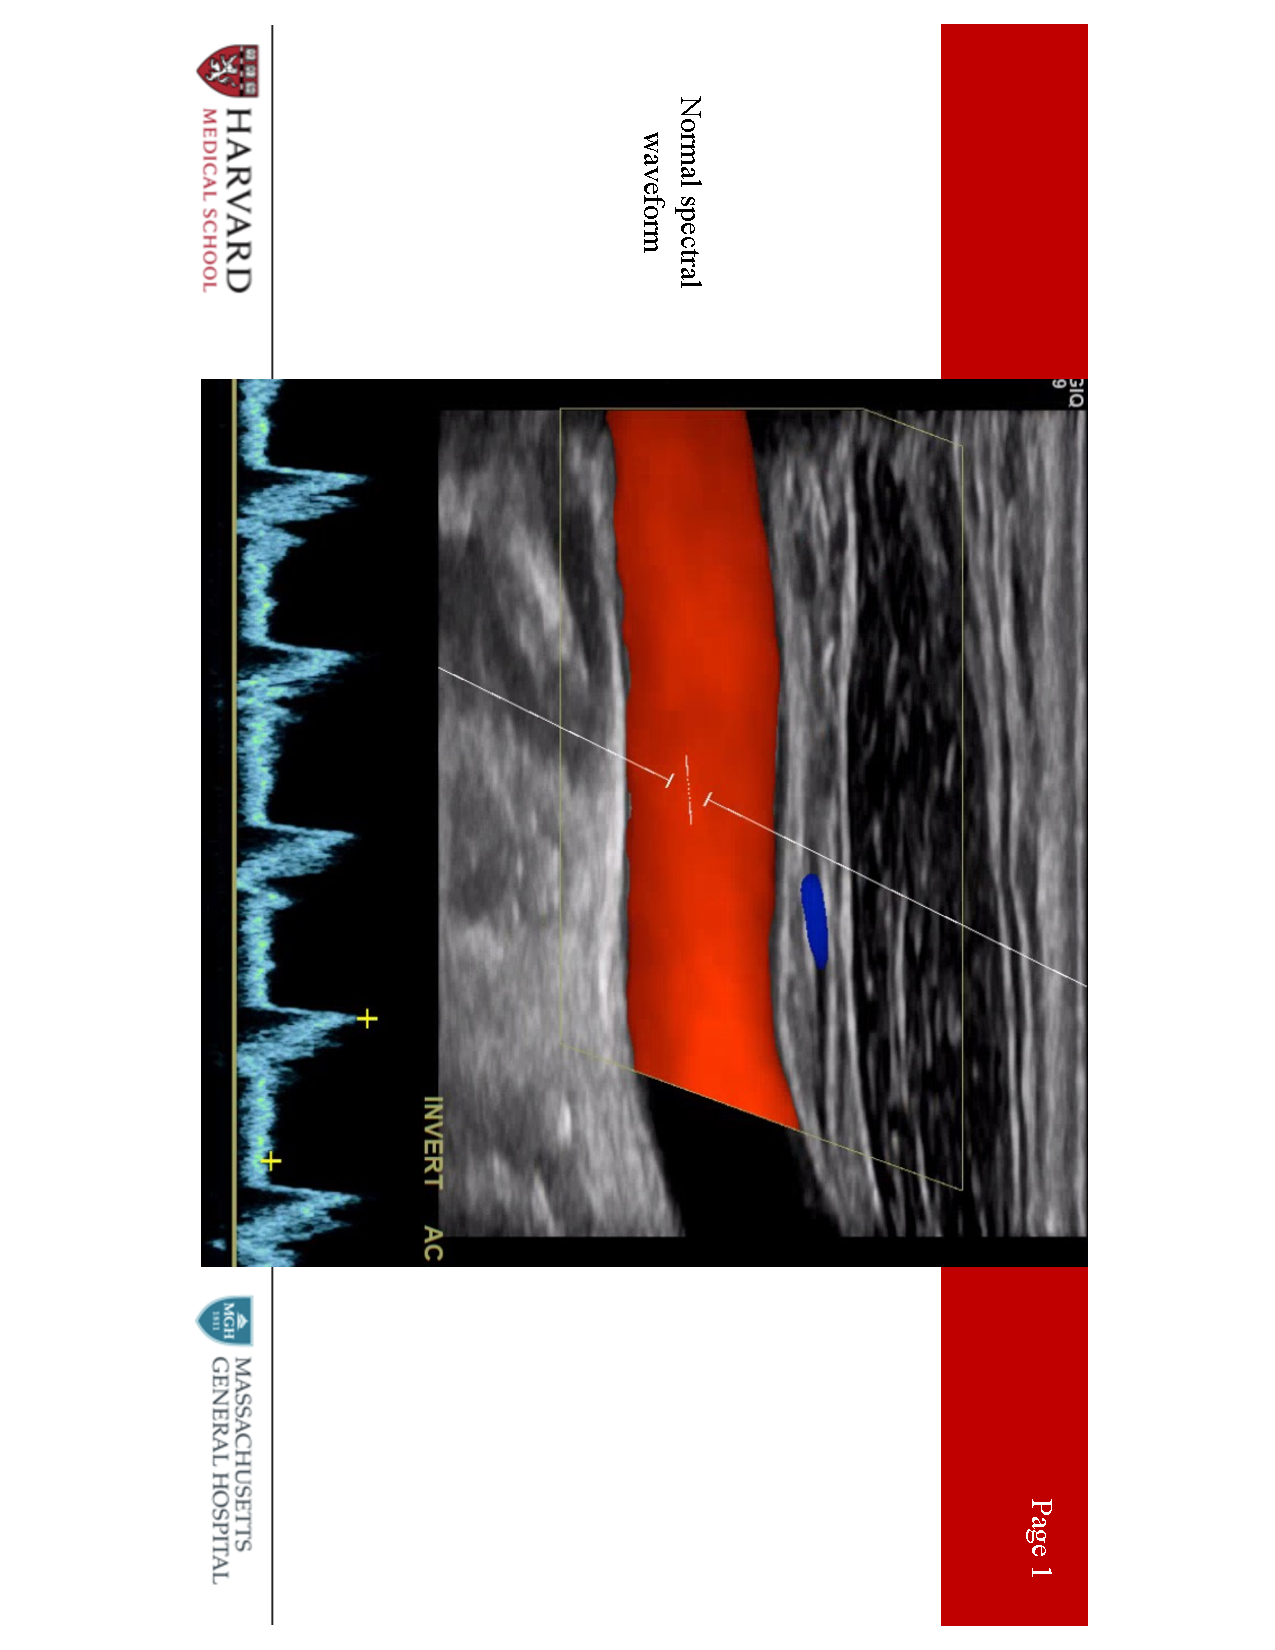
\includegraphics[width=10in]{images/vasc_lab/Slide2}

\underline{Low vs high resistance waveforms:}

Waveform profiles change depending upon the nature of the distal
vascular bed being supplied. Organs like the brain, kidneys, liver, and
spleen have constant high metabolic demand, and are therefore low
resistance vascular beds. Waveforms for arteries supplying these organs
demonstrate constant forward flow throughout the cardiac cycle because
the distal bed being supplied has low resistance leading to high
end-diastolic flow.

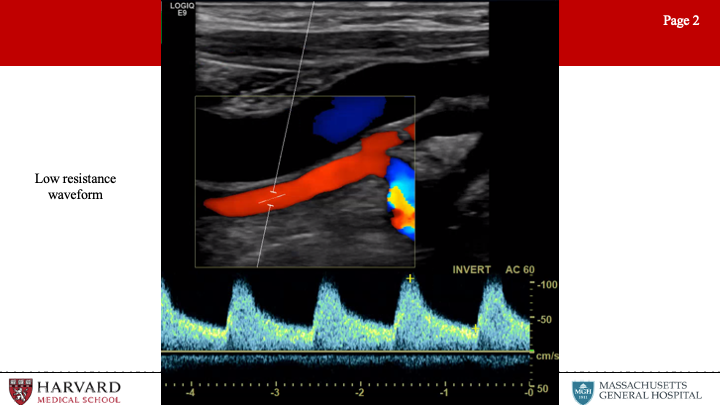
\includegraphics[width=10in]{images/vasc_lab/Slide3}

This would also be seen in the postprandial SMA. In contrast, high
resistance waveforms are seen for arteries supplying resting peripheral
muscles, fasted mesenteric beds (such as the~fasting~SMA), and the
External carotid artery. High resistance waveforms are characterized by
triphasic morphology (preprandial~ SMA or ECA).

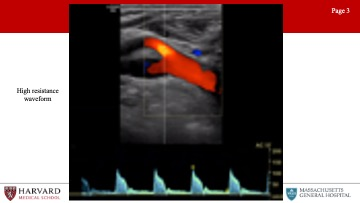
\includegraphics[width=10in]{images/vasc_lab/Slide4}

That is, sharp peaks, early diastolic flow reversal, brief forward flow
from elastic recoil of the artery, and then no flow during the remainder
of the diastolic phase.

\textbf{How does flow-limiting stenosis change the waveform?}

First let's define~\textbf{Stenosis:}~A hemodynamically significant stenosis
(area reduction \textgreater50\%) will result in a doubling of velocity from the
inflow segment to the area of maximal stenosis (velocity ratio \textgreater{} 2).

Now what do waveforms look like AFTER a flow-limiting stenosis?

\underline{Tardus et parvus}~refers to a pattern of Doppler ultrasound
spectral waveform resulting from arterial stenosis. The tardus et parvus
waveform is delayed with prolonged systolic acceleration (tardus) and
diminished with a small systolic amplitude and rounded systolic peak
(parvus). This phenomenon is observed downstream from the site of
stenosis. Tardus parvus in the CFA? Upstream (iliac) stenosis. Tardus
parvus in the brachial artery? Upstream (subclavian or axillary)
stenosis.

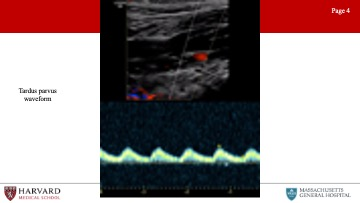
\includegraphics[width=10in]{images/vasc_lab/Slide5}

\textbf{So what will the waveform look like BEFORE a flow-limiting stenosis?}

\underline{Distal stenosis:} Distal occlusive disease will result in a high
resistance waveform, with absent diastolic flow. (Image 5: Distal
stenosis with absent diastolic flow)

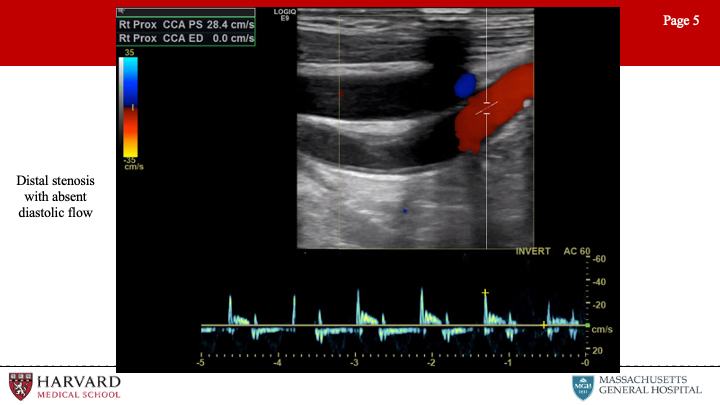
\includegraphics[width=10in]{images/vasc_lab/Slide6}

Now that we've covered the basics, let's move through by organ-~system
high-yield vascular lab studies, findings, and pathologies.We'll start
with the extracranial evaluation, a highly-tested area of vascular
ultrasonography.

\underline{\textbf{Extracranial:}}

What does a typical extracranial evaluation involve?

-~~~~~~~Examine CCA (2 views), ICA (2 views), ECA, vertebral arteries

What are normal ICA and ECA waveforms?

-~~~~~~~\textbf{Normal ECA vs ICA waveform:}

The external carotid artery waveform reflects a high resistance vascular
bed. This means minimal diastolic flow. Conversely, the ICA waveform
reflects a low resistance vascular bed with antegrade diastolic flow.
(Image 6: normal ICA waveform)~This makes sense, as the ICA is supplying
the brain while the ECA is supplying the face. Intuitively, the common
carotid artery~ is a mixture of the ICA and ECA waveform morphologies.
Like the ICA with forward flow throughout diastole, but less as compared
to the ICA due to the high resistance influence of the ECA.

Another way of differentiating the external and internal carotid
arteries is the ``temporal tap''. Tapping on the superficial temporal
artery (a branch of the ECA) will be transmitted as small pulsations in
the diastolic component of the external carotid artery. (Image 7: ECA
waveform with~temporal tap)

Can you talk about diagnostic criteria for ICA stenosis?

-~~~~~~~\textbf{Parameters for ICA stenosis:}

These are a few numbers that are (unfortunately) essential to memorize
for the VSITE and RPVI.

Although criteria differ between guidelines, the Carotid Consensus
Criteria, define ICA stenosis \textgreater= 70\% as a peak systolic velocity \textgreater=
230 cm/sec, EDV \textgreater{} 100 cm/sec, and ICA/CCA ratio \textgreater{} 4.0. Of note,
post-stenting criteria vary from pre-stenting criteria. Stenosis
criteria are not clearly defined for the CCA or ECA. (Image 8: stenotic
ICA)

When is surgery indicated for ICA stenosis?

-~~~~~~~\textbf{Parameters for when surgery indicated}:

Asymptomatic Carotid Atherosclerosis Study (ACAS) \textgreater60\% stenosis
asymptomatic, NASCET \textgreater50\% stenosis symptomatic

Let's talk about other pathologies that can be visualized on
extracranial ultrasound:

-~~~~~~~\textbf{Pathologies:}

Stenosis (plaque), dissection (flap), aneurysms (rare), occlusion (no
flow, do not operate), carotid body tumor (splaying of ECA/ICA, fed by
ECA branches), FMD.

FMD is frequently encountered on the VSITE/RPVI. How would this appear
on the exams?

-~~~~~~~\textbf{Fibromuscular dysplasia}~of the internal carotid arteries
affects women more commonly than men. Duplex findings show a ``chain of
lakes'' appearance, demonstrative of multiple septa and small aneurysms.
Velocity elevations and increased turbulence in the waveform patterns is
typically found on Doppler interrogation.~(Image 9: Fibromuscular
dysplasia in the ICA)~How to treat? Aspirin if asymptomatic, POBA if
symptomatic.

Are there other frequently tested pathologies demonstrated on
extracranial exam?

-~~~~~~~\textbf{Subclavian steal:}~Subclavian steal occurs when a proximal
subclavian stenosis or occlusion leads to reversal of vertebral artery
flow. This causes ``stealing'' of~ blood from the posterior cerebral
circulation, and presents as vertebrobasilar insufficiency. How does
this look on duplex? Normal vertebral flow looks very similar to ICA:
antegrade low resistance waveforms with constant forward flow throughout
the cardiac cycle. As subclavian stenosis progresses, one can see
mid-systolic velocity decelerations ('bunny ears'') , and with severe
steal, there is a complete reversal of flow in the vertebral artery
towards the arm rather than towards the brain. (Image 10: subclavian
steal as demonstrated by mid-systolic decelerations in the vertebral
artery)

-~~~~~~~\textbf{Innominate stenosis:}~A phenomenon that is related to this,
is innominate stenosis. Here again the patient will present with
vertebrobasilar insufficiency, indicative of diminished vertebral
antegrade flow, but additionally will experience right hemispheric
insufficiency secondary to diminished R ICA antegrade flow. The
right-side duplex will demonstrate flow reversal in the vertebral
artery, abnormal waveforms in the subclavian, as well as steal pattern
waveforms in the common and internal carotid arteries. The common
denominator for all of these findings is significant disease in the
innominate artery.

~

So that covers extracranial vascular lab evaluation. What about
intracranial? This is less frequently tested, so we will discuss just a
brief overview of views and some of the more commonly tested
pathologies.

\underline{\textbf{Intracranial:}}

-~~~~~~~Three primary views: temporal, foraminal (occipital), orbital
views

-~~~~~~~~~~\textbf{Temporal view:}~Used to interrogate PCA, ACA, MCA, and
ICA.

The~MCA, ICA and PCA flow direction is towards the probe, the~, The
ACA~flow direction~is AWAY.

-~~~~~~~~~~\textbf{Occipital view:}~Basilar and vertebral arteries (both
away).

-~~~~~~~~~~\textbf{Orbital view:}~Ophthalmic and ICA

-~~~~~~~Arteries differentiated by depth. MCA 3-6 cm, everything else
deeper.

What are some frequently tested pathologies that are identified on TCD?

-~~~~~~~\textbf{Indications often tested:}

-~~~~~~~\textbf{MCA spasm (severe PSV\textgreater200)}: Can be seen in sickle cell
disease with studies indicating a strong correlation between mean
velocities of \textgreater200cm/s and the rate of stroke in children with sickle
cell disease. With blood transfusions, stroke risk can be reduced from
\textgreater10\% to \textless1\% per year.\textsuperscript{\href{https://paperpile.com/c/NdGHca/WRZA}{1}}

-~~~~~~~\textbf{Cerebral ischemia during CEA:}~Comparing transcranial Doppler
sonography, near-infrared spectroscopy, stump pressure measurement, and
somatosensory evoked potentials, cerebral ischemia was most accurately
predicted by the percent change in transcranial Doppler detected middle
cerebral artery velocity. Detection of a greater than 50\% drop in middle
cerebral artery velocity using transcranial Doppler is 100\% sensitive
for detecting cerebral
ischemia.\textsuperscript{\href{https://paperpile.com/c/NdGHca/m4Pw}{2}}

-~~~~~~~TCD can also demonstrate microemboli (high spikes on spectral
doppler) during CEA

~

Having covered head and neck vasculature, let's move on to peripheral
vasculature. This is a huge area both on the VSITE/RPVI and in practice.
In this section we'll cover first the upper, then the lower extremity
vasculature.

So first, what are characteristics of waveforms in the peripheral
vasculature?

\underline{\textbf{Peripheral:}}

-~~~~~~~Normal waveforms are indicative of high resistance distal beds,
so we would expect triphasic waveforms

What are normal arterial parameters in the upper extremities?

\underline{\textbf{Upper Extremity:}}

-~~~~~~~\textbf{Normal parameters:}~Normal pressure gradient between the
right and left brachial pressures is \textless20 mmHg. Normal finger pressure
is \textgreater80\% of the ipsilateral brachial systolic pressure. So a normal
digital brachial index is \textgreater=0.80. A gradient between digits of \textgreater15
mmHg is considered abnormal.~

~

Let's talk about some of the most frequently tested pathologies,
starting with arterial TOS.

-~~~~~~~~~~\textbf{Arterial TOS:}~Results from compression of the subclavian
artery at the level of the first rib within the scalene triangle.
Arterial TOS testing is done by placing a sensor, most often
photoplethysmography (PPG), on one finger of each hand, recording the
resting waveforms and then recording while during maneuvers to evoke
arterial compression in the thoracic outlet.

Can you tell us a little more about PPG testing?

-~~~~~~~~~~\textbf{Photoplethysmography (PPG)}~uses an infrared light to
illuminate superficial tissue. The reflection is received by a
photosensor, and amplitude of the reflected light is proportional to the
volume of red blood cells in the sample area. A normal digital arterial
PPG has a brisk upstroke with a narrow systolic peak, and a dicrotic
notch on the downslope during diastole (Image 11: normal PPG).~Digital
PPGs change with progression of peripheral vascular disease. The first
changes are a loss of amplitude and loss of the dicrotic notch. More
advanced disease~findings include a flattened systolic peak and a
prolonged upstroke. Significant arterial TOS is suggested when there is
a loss or persistent flattening of the digit waveforms during any of the
positional changes that can compress the subclavian artery (either with
the clavicle, first rib and scalene muscle). However, it should be noted
that up to one-third of patients without arterial TOS may have some
degree of subclavian artery compression with positional maneuvers.

What are other diseases affecting the upper extremity?

-~~~~~~~\textbf{Raynaud's:}~Vasospastic disorder characterized by temporary
vasospasm. Diagnosis may be assisted by decrease in digital waveforms
with immersion of the hand in cold water.

-~~~~~~~~~~\textbf{Thromboangiitis obliterans:}~Is a segmental
non-atherosclerotic inflammatory disorder characterized by
microthrombosis that primarily involves the small- and medium-sized
arteries. Ultrasonography may demonstrate the classical ``corkscrew''
collateral development at the level of occlusion. TA has a male
predominance and first line treatment is smoking cessation.

~

Before we segue to the lower extremities, this is a good time to discuss
an entity frequently tested on the VSITE, and that constitutes for many
vascular surgeons a notable portion of their practice, and that is
hemodialysis access, and specifically fistulas.

\underline{\textbf{Fistulas:}}

Ultrasound is one of the key modalities used in identifying suitable
anatomy for fistula placement, suitability of a fistula for dialysis,
and finally complications of fistulas.

So first, assessment for fistula placement:

-~~~~~~~\textbf{Assessment for fistula placement:}

-~~~~~~~The optimal configuration for an AVF is determined on the basis
of vein mapping and noninvasive studies. Veins should measure \textgreater3 mm in
diameter (\textgreater2.5 mm may be acceptable, as veins are likely to dilate under
anesthesia), and there should be no arterial inflow stenosis or venous
outflow stenosis. Duplex ultrasound arterial imaging can be performed at
the same time as vein mapping and can provide important predictors of
fistula maturation, such as arterial diameter and flow. The minimal
arterial lumen diameter is 2 mm.

How can we tell if a fistula is ready to be used for hemodialysis
access?

-~~~~~~~~~~\textbf{Assessment for fistula suitability for dialysis:}~Rule of
6's: At six weeks post-creation the diameter of the fistula should be at
least 6 mm and the depth no more than 0.6 cm. The flow rate should be at
least 600mL/min, and the length of the fistula should be 6 cm to allow
for a successful two-needle dialysis.

What do normal fistula spectral waveforms look like?

-~~~~~~~~~~\textbf{Waveform:}~The arterial waveform should demonstrate very
low resistance throughout diastole. End diastolic velocity should be one
half to two thirds of peak systolic velocity in a well-functioning
fistula. As a side note, this is also what one would see in an
iatrogenic arteriovenous fistula, as between the femoral artery and
vein.

Let's discuss commonly encountered complications and pathologies
identified in association with fistulas:

-~~~~~~~\textbf{Pathology:}

-~~~~~~~~~~\textbf{Pseudoaneurysms:}~Pseudoaneurysms commonly occur when a
puncture fails to seal and the blood is contained by the surrounding
soft tissue. As in other locations, pseudoaneurysms are defined on
imaging by a communicating neck between the arterial vessel and
pseudoaneurysmal sac with ``to-and-fro'' waveform at duplex. While small
pseudoaneurysms can be managed without intervention or surgery, larger
pseudoaneurysms, pseudoaneurysms associated with infection or overlying
skin changes or bleeding may require excision and repair.

-~~~~~~~~~~\textbf{Steal syndrome:}~Hemodialysis-related steal, also known as
access-related hand ischemia, which may occur in over half of all
patients undergoing access creation. Steal is characterized by
retrograde diastolic flow distal to the donor artery. Of note, reversal
of flow in and of itself is not sufficient to cause distal ischemia with
an intact palmar arch. This is commonly seen after access creation and
represents physiologic steal phenomenon, rather than symptomatic steal
syndrome. Digital pressures \textless60 mm Hg are highly sensitive and specific
for predicting steal. Patients who have no symptoms (Grade 1
access-related hand ischemia), may be closely monitored without any
intervention. How do we treat more severe steal? Flow rate measurements
of the fistula can help determine the optimal treatment (banding,
revision using distal inflow, distal revascularization with interval
ligation, proximalization of arterial inflow or ligation of the
fistula).

So steal can occur in the context of high fistula output, can we talk a
bit about low fistula flow, as from stenosis?

-~~~~~~~~~~\textbf{Central venous stenosis:}~Venous outflow stenosis is the
most common reason for arteriovenous graft failure. A low flow rate
results in recirculation during the dialysis session. Venous obstruction
manifests as arm swelling, and with central venous stenosis may present
with collateral development over the upper extremity and chest wall.

-~~~~~~~~~~\textbf{Stenosis of fistula:}~Arterial and mid-graft stenosis can
also cause complications, but are less common than venous stenosis.
Stenosis on imaging will be represented by narrowing of luminal diameter
on b-mode ultrasound, high-resistance waveform proximal to the stenosis,
and tardus parvus waveform distal to the stenosis.

~

Awesome. So now that we've briefly covered fistulas, let's return to
peripheral vasculature, this time in the lower extremities.

~

\underline{\textbf{Lower Extremity:}}

~

Can you please tell us about some of the diagnostic modalities that are
used to examine perfusion in the lower extremities?~

-~~~~~~~~~~\textbf{Diagnostic Modalities:}

-~~~~~~~~~~\textbf{ABIs:}~Ankle-brachial index measurement requires
calculating the ratio of the highest ankle systolic pressure (posterior
tibial artery or dorsalis pedis) over the highest brachial systolic
pressure. Regardless of whether you're doing the R or L ABI, use the
higher arm pressure for both ratios. Normal ABI \textgreater0.9, severe disease
indicated by ABI\textless0.5, and CLI by ABI\textless0.3. The ankle-brachial index in
diabetic patients is frequently unreliable due to incompressibility of
the tibial vessels at the level of the cuff secondary to calcification.
Consequently, toe pressures are mandatory in all patients with diabetes
mellitus. Normal TBI\textgreater0.7.

-~~~~~~~\textbf{TcPO2:}~When there is significant tissue loss, preventing TBI
measurement, another option is transcutaneous oximetry
(TcPO2).~~Transcutaneous oximetry is a non-invasive method of measuring
the tissue partial pressure of oxygen through a heated sensor on the
skin. A TcPO2 value of 40 mmHg is the critical value below which wound
healing is impaired and ischemia develops.

Are there other non-invasive ways of determining extremity perfusion?

-~~~~~~~~~~\textbf{PVRs:}~Pulse volume recordings. Normal PVR waveforms have
a rapid upstroke, sharp peak, prominent dicrotic notch and downslope.
Typically 4 cuffs. High thigh cuff should be 30\% greater than brachial
pressure, hence a thigh-brachial index of 1.3 is normal. However,
ABI/PVRs may not demonstrate significantly abnormal values/waveforms in
individuals with single level disease. (Image 12: PVRs- normal right leg
and abnormal left leg)

-~~~~~~~~~~\textbf{Exercise Test:}~During exercise testing, patients are
placed on a treadmill after baseline resting ABIs are measured. The
patient is then asked to walk for 5 minutes or until physical discomfort
requires test cessation. The point when a patient stops is defined as
the absolute claudication distance. Diagnostic criteria for a positive
test include a drop-in ankle pressure of greater than 20 mmHg from
baseline, drop in ABI greater than 0.2 from baseline, or inability of
ankle pressures to return to baseline after 3 minutes.

So just to briefly summarize, what are parameters associated with poor
wound healing?

-~~~~~~~\textbf{Parameters associated with poor wound healing:}~Considering
these various testing modalities, what are factors associated with poor
likelihood of wound healing? An ankle pressure \textless50 mmHg, ABI \textless{} 0.40,
TcPO2 \textless20 mmHg, or a toe pressure \textless20 mmHg are considered predictive
of non-healing.

Ultrasound is frequently used for graft surveillance. Can you talk about
graft surveillance parameters?

-~~~~~~~\textbf{Restenosis/Graft surveillance:}~Suggested ultrasound
surveillance bypass graft begins immediately after surgery and then
continues at 3, 6, and 12 months and then every 6 to 12 months
thereafter. A velocity ratio (Vr) is defined as the peak systolic
velocity (PSV) at the site of a stenosis divided by the PSV in a normal
vessel segment proximal to the stenosis. The highest risk for graft
thrombosis, and highest cause for concern is suggested by PSV \textgreater300
cm/s, Vr \textgreater3.5, a graft flow velocity \textless45 cm/s or a drop in ABI
\textgreater0.15.\textsuperscript{\href{https://paperpile.com/c/NdGHca/OBYf}{3}}

Let's talk about pathologies frequently encountered in the lower
extremities:

-~~~~~~~\textbf{Pathologies:}

-~~~~~~~~~~\textbf{Pseudoaneurysms (particularly femoral):}~Gray-scale
ultrasonography demonstrates a hypoechoic cystic structure adjacent to
an arterial supply. Color Doppler typically demonstrates a ``yin-yang
sign'' within the pseudoaneurysm sac. The hallmark ultrasound sign is
identification of a neck between the sac and the feeding artery with a
``to-and-fro'' spectral Doppler waveform measured at the neck. This
represents the flow in and out of the PSA during systole and diastole
(Image 13:~pseudoaneurysm with a ``yin-yang sign'').

-~~~~~~~~~~\textbf{Dissections:}~Characteristic ultrasound findings on color
Doppler include a parallel blood-flow channel that separates the true
and false lumen (Image 14:~dissection). Of note, if the false lumen is
filled by a thrombus, it may not distinguishable from an intramural
hematoma or noncalcified plaque

There are several disease pathologies that are frequently tested
relating to the popliteal fossa. Can you talk briefly about these?

-~~~~~~~~~~\textbf{Adventitial cystic disease:}~This is a rare (but often
tested) pathology. Adventitial cystic disease is a nonatherosclerotic
etiology of claudication, most often affecting the popliteal artery in
the lower extremity and leading to stenosis or occlusion. Duplex imaging
of the popliteal artery will demonstrate an
anechoic~\emph{intraluminal}~region with a smooth contour and stenosis
documented by velocity increase on spectral doppler~(Image 15:
adventitial cystic disease).~~This is not to be confused with a

-~~~~~~~\textbf{Bakers Cyst:}~which is a benign, cystic structure found in
the popliteal fossa and arising from the joint capsule. Flexion of the
knee may result in compression of the popliteal artery by the cyst. On
b-mode ultrasound, a well-defined, anechoic~ cystic structure with a
`neck' extending into the joint space between the semimembranosus tendon
and the medial head of the gastrocnemius will be identified (Image
16:~Baker's cyst).

-~~~~~~~\textbf{Popliteal entrapment syndrome:}~decrease in ABI or loss of
distal pulses with passive dorsiflexion or active plantar flexion of the
foot caused by compression of the popliteal artery by the gastrocnemius.

Now that we've covered the extremities, let's discuss ultrasound
evaluation of abdominal vasculature.

~

\underline{\textbf{Abdominal:}}

First, let's discuss the aorta and AAAs.

-~~~~~~~\textbf{Aortic Pathologies:}

-~~~~~~~\textbf{AAA:}~Ultrasound screening of a AAA is non-invasive,
accurate, and cost-effective. Sensitivity of 98\% and specificity of 99\%
for AAA diagnosis. Size criteria for AAA repair is 5.5 cm men, 5.0-5.5
cm in women, measured outer~wall to outer~wall cross-sectional diameter.

Can ultrasound be used for graft surveillance s/p EVAR?

-~~~~~~~\textbf{S/p EVAR:}~Surveillance color duplex ultrasound is safe if CT
imaging at 1 year exhibits no sac growth, graft migration, or endoleak
(or stable type II endoleak). Can detect endoleaks, sac expansion, and
limb occlusion. Migration difficult to assess given challenge of renal
arteries visualization in a long axis view of the aorta.

What other pathologies can be identified on ultrasound evaluation of the
abdomen?

-~~~~~~~\textbf{CIA aneurysms:}~SVS defines CIA aneurysms as any permanent,
localized dilatation of the iliac artery \textgreater1.5 cm in diameter (diameter
1.5x the normal diameter)

-~~~~~~~\textbf{Para-anastomotic pseudoaneurysms:}~As previously discussed
(reported in up to 0.5\% to 10\% of cases)

-~~~~~~~\textbf{Penetrating aortic ulcers:}~Describes an ulcerating
atherosclerotic lesion that penetrates the intima and progresses into
the media. Associated with atherosclerotic plaque on ultrasound

-~~~~~~~\textbf{Dissections:}~(as already discussed) a dissection flap is
usually identified and color flow demonstrates dual channels (true and
false lumens). Turbulent flow patterns are frequently encountered.

So far we have steered clear of the mesenteric vasculature. But this is
an area frequently encountered on exams. Let's start with mesenteric
vessel stenosis.

-~~~~~~~\textbf{Mesenteric Pathologies:}

-~~~~~~~\textbf{Celiac and SMA stenosis:}~May present as chronic mesenteric
ischemia.~PSV \textgreater275 cm/s in the SMA or \textgreater200 cm/s in the celiac artery
indicates \textgreater=70\% stenosis. Normal SMA Doppler waveforms in the fasting
patient show high resistance waveform, PSV \textless275 cm/s and no spectral
broadening. In the postprandial state, the waveform becomes low
resistance, with a slightly increased PSV and little to no spectral
broadening. Significant SMA stenosis may be differentiated by the
presence of spectral broadening and elevated PSV and EDV. Distal to the
stenosis, one would expect a tardus parvis waveform. EDV \textgreater45 in SMA or
\textgreater55 in celiac are predictive of stenosis (would expect higher diastolic
flow in celiac trunk given low resistance vascular bed of liver and
spleen).

What other mesenteric vessel pathologies may be identified on vascular
ultrasound?

-~~~~~~~\textbf{Dissections:}~Rare without concomitant aortic dissection.

-~~~~~~~\textbf{Aneurysms:}~Rare. Repair \textgreater2 cm celiac, hepatic, SMA
aneurysms and \textgreater3 cm splenic and renal.

-~~~~~~~\textbf{Median arcuate ligament syndrome:}~MALS can cause
significantly elevated velocities at the origin of the celiac artery.
Testing is for reversible mechanical compression, as opposed to a fixed
lesion from atherosclerotic disease. During deep inspiration or in the
upright position, celiac velocities should normalize if stenosis is
secondary to MALS.

Ok, so I recognize that we are jumping ahead here discussing venous
circulation, but as this represents another component of a mesenteric
vascular exam, let's discuss portal venous ultrasonography.

-~~~~~~~\textbf{Portal vein:}~Normal portal venous flow is hepatopetal
(toward the liver), whereas abnormal portal venous flow is hepatofugal
(away from the liver). (The root ``fugua'' means to flee, or flight). Flow
should be in the same direction as the hepatic artery. Other
abnormalities that may be visualized are portal vein thrombosis (often
associated with portal venous hypertension in patients with chronic
cirrhosis, hepatitis, or hepatocellular carcinoma). Acute portal vein
thrombosis on ultrasound demonstrates dilatation of the portal vein with
hypoechoic intraluminal thrombus. Chronic portal vein thrombosis is
characterized by a contracted vein with heterogeneous/hyperechoic echoes
and may be associated with collateral formation.~ Can also assess for
hepatic artery stenosis/thrombosis and for functioning of TIPS
(transjugular intrahepatic portosystemic shunt).

Awesome, and so before jumping fully into venous circulation, let's
complete our discussion of abdominal ultrasound evaluation with a
discussion of the renal vasculature.

-~~~~~~~\textbf{Renal Pathologies:}~ostial (atherosclerotic) vs mid-artery
(FMD)

-~~~~~~~\textbf{Atherosclerotic stenosis:}~PSV\textgreater200 cm/s predictive of \textgreater60\%
stenosis. Renal artery-to-aortic PSV ratio (RAR) \textgreater3.5 also correlates
with a \textgreater60\% stenosis. The renal resistive index (RRI) is calculated as
the RA PSV-EDV/PSV. The RRI (\textgreater0.8) is an indicator of intrinsic
parenchymal renal disease.

-~~~~~~~~~~\textbf{FMD:}~As discussed for the carotids, FMD manifests as
beaded lesions in medium and small arteries, with the renal arteries the
most commonly affected. Ultrasound demonstrates increased PSV in the mid
and distal renal artery. Stenoses in the mid and distal renal artery are
suggestive of FMD, atherosclerotic disease is primarily ostial in
nature.

So far we've predominantly focused on arterial findings, let's discuss
venous vascular lab evaluations:

\underline{\textbf{Venous:}}

-~~~~~~~\textbf{Venous Exam:}~Uses a linear transducer. Complete deep venous
reflux duplex examination includes color and pulsed wave spectral
doppler imaging. Spontaneous Doppler waveforms as well as provocative
maneuvers are recorded in the common femoral, femoral, popliteal, and
tibial deep veins. Superficial veins (GSV, SSV, and perforator veins)
are evaluated with provocative maneuvers to test valve competency.
Diameters are also included for superficial veins. Transverse B-mode
images are used for vessel compression (as when looking for thrombus) to
ensure that the vein is fully compressible under probe pressure as
opposed to simply slipping out of view, as may occur in longitudinal
views. Reflux exam should be performed with a patient standing, with
assessment performed on the non weight-bearing leg.

We've talked extensively about normal arterial waveforms; what do normal
venous waveforms look like?

-~~~~~~~\textbf{Normal venous waveforms:}~Normal flow patterns of iliac and
femoral veins demonstrate phasicity and should augment with distal
compression. In the upper extremity central veins, doppler waveforms
normally demonstrate pulsatility and phasicity.

What does this mean? Pulsatility, phasicity, and augmentation?

\textbf{Pulsatility:}~Refers to changes in the venous waveform in accordance
with the cardiac cycle. Pulsatility is normal in the upper extremity
veins central veins, given their proximity to the heart (Image 17:
pulsatility in an~upper extremity vein). This is an abnormal finding in
the lower extremity veins, and may be a sign of pulmonary hypertension,
right heart failure, or tricuspid regurgitation.

\textbf{Phasicity:} (also called respiratory phasicity) is variation in the
waveform with respiration~(Image 18: phasicity in a vein). This results
from increasing and decreasing intrathoracic pressures secondary to
respiration. Phasicity is an indicator of a patency proximal to the
point of measurement. So if we see lack of phasicity (continuous flow)
in the left femoral vein but normal phasicity in the right, we would be
concerned for left iliac vein occlusion or stenosis. If we saw absence
of phasicity (continuous flow) in the bilateral femoral veins, we would
be concerned for IVC obstruction or stenosis.~

\textbf{Augmentation:}~Distal compression that augments forward flow (Image
19: augmentation in a lower extremity vein). For example, if we are
measuring flow at the femoral vein and we squeeze the calf and we see
augmentation in the waveform, this indicates lack of occlusion in the
venous system from the knee to the probe.

What are venous pathologies that are commonly tested/encountered?

-~~~~~~~\textbf{Pathologies:}~2 primary pathologies are reflux and
obstruction

-~~~~~~~\textbf{Reflux:}~Venous reflux due to valvular incompetence is best
assessed with duplex scanning in the upright position. Reflux in the
common femoral vein and the saphenofemoral junction may be elicited with
a Valsalva maneuver (which increases intra-abdominal pressure), but
release of a pneumatic cuff compression is a more reproducible method.
Reflux is identified as reverse flow - that is, away from the heart -
following valsalva or release of the compression cuff (Image 20: reflux
in a lower extremity vein). Consensus guidelines suggest a cutoff value
of 1 second for abnormally reversed flow (reflux) in the femoral and
popliteal veins and of 0.5 seconds for the great saphenous vein, small
saphenous vein, tibial, and deep femoral veins.

-~~~~~~~\textbf{Perforator veins:}~Perforator veins connect the deep and
superficial venous systems, penetrating the deep fascia overlying the
muscle.~ Size \textgreater3.5 mm and reflux \textgreater350 ms (deep to superficial) is
associated with perforator reflux. Pathological perforator = in
association with a healed or non-healed ulcer.

What are some other examples of reflux?

-~~~~~~~\textbf{Ovarian vein reflux:}~The ultrasound evaluation of pelvic
congestion syndrome is performed in steep reverse Trendelenburg and
standing positions with a low-frequency probe. Reflux is identified
during the Valsalva maneuver. There are no validated criteria for the
duration of reflux. Rather, an ovarian vein diameter \textgreater6 mm is
considered significant.

-~~~~~~~\textbf{May Thurner:}~Also known as iliac vein compression syndrome,
refers to a chronic compression of the left~\href{https://radiopaedia.org/articles/common-iliac-vein?lang=us}{common iliac
vein}by the
overlying right~\href{https://radiopaedia.org/articles/common-iliac-artery?lang=us}{common iliac
artery}~(CIA),
with or without~\href{https://radiopaedia.org/articles/deep-vein-thrombosis?lang=us}{deep venous
thrombosis}.
Notably, patients present with unilateral (left) lower extremity edema
and pain, varicosities, DVT or venous ulcers. Intravascular ultrasound
will demonstrate \textgreater50\% stenosis of the iliac vein from compression.
Distal waveforms will demonstrate absence of phasicity if
obstruction/stenosis is severe with continuous flow.

Ok, let's transition from reflux to thrombosis:

-~~~~~~~\textbf{Thrombosis:}~Characteristics of acute thrombus are an
echolucent and incompressible thrombus in a thin-walled vein with
significant distension~(Image 21: non-compressible vein positive for
DVT).~Acute thrombus typically causes the vein to dilate with a diameter
greater than the diameter of the adjacent artery. Venous wall
thickening/scarring, a contracted vein, recanalization, and
collateralization is found in chronic thrombosis.

Let's discuss 2 Specific examples of venous thrombosis: VTOS and EHIT

\textbf{Venous TOS:}~Venous thoracic outlet syndrome is thrombosis or severe
stenosis of the subclavian or axillary veins secondary to chronic
extrinsic mechanical compression. Repetitive injury to the subclavian
vein at the level of the costoclavicular space results in chronic injury
to the veins. Venous duplex may show a dilated, non-compressible vein
consistent with an acute subclavian vein DVT, or lack of
pulsatility/phasicity if obstruction/stenosis is more centrally located.

\textbf{EHIT or Endovenous Heat Induced Thrombosis:}~S/p endovenous thermal
ablations (RFA or laser ablation) of the GSV. 4 Grades: Grade 1 is
thrombus in the GSV up to the level of the CFV. If \textless{} 50\% of the CFV
lumen is involved this is EHIT grade 2. EHIT grade 3 is extension into
the CFV occupying \textgreater50\% of the lumen and grade 4 is occlusion of the CFV
(Image 22: EHIT Grade 2). EHIT grades 3-4 are typically treated with
anticoagulation to reduce risk of PE. To minimize the risk of EHIT, the
catheter should be positioned at least 2 cm from the saphenofemoral
junction.

~

Finally, let's wrap up this episode with a discussion of imaging
artifacts. These are frequently encountered and tested in vascular
ultrasound, and it is important to recognize imaging artifacts in order
to prevent incorrect interpretation.

\underline{\textbf{Artifacts:}}

-~~~~~~~\textbf{Acoustic shadowing:}~Shadowing on an ultrasound image is
characterized by a signal void behind structures that strongly absorb,
reflect, or refract ultrasonic waves (Image 23:~acoustic shadowing).
Practically speaking, this most typically occurs deep to strongly
reflective surfaces such as calcified plaques, and appears as a ``dark
area'' beneath the plaque.~\textbf{Acoustic enhancement}~is essentially the
inverse situation, and appears as a ``bright area'' deep to structures
that transmit ultrasound waves exceptionally well. This can happen deep
to fluid-filled structures such as cysts.

-~~~~~~~\textbf{Mirroring}: A mirror-image artifact is caused by
reverberation of ultrasound and shows structures that exist on one side
of a strong reflector as also being present on the other side of the
reflector (Image 24: mirror-image artifact).This is often seen around
the pleura and the diaphragm, due to the strong reflection of ultrasound
from the air-filled lung. These artifacts can occur in both B-mode
imaging where you see the mirrored image and Doppler, in which you see
the mirrored waveform.

-~~~~~~~\textbf{Refraction:}~A refraction artifact is the result of
ultrasound waves passing through tissues with different propagation
velocities (such as air and water) and causes a structure to be
improperly positioned laterally in the image. This is the phenomenon
that results in a straw appearing bent when in a glass of water.

-~~~~~~~\textbf{Speed artifact:}~Depth determination by an ultrasound machine
is based on calculations using an average propagation velocity of sound
in soft tissue of 1540 m/s. If the ultrasound wave passes through a
medium at a different speed than predicted by the machine, an inaccurate
image depth will be displayed. If the ultrasound passes less quickly
through the material than soft tissue (as occurs in air or fluid), then
the image will be displayed deeper than the true depth. In practical
application, this is what causes a ``bayonet'' sign, or apparent bending
of a needle when it passes from soft tissue into a cystic structure.

-~~~~~~~\textbf{Inappropriate color gain:}~Overly gained images will show
``speckling'' in areas in which no flow is present (such as in soft
tissue) (Image 25: color over-gaining). Under-gaining will result in
reduced sensitivity to low velocity flow.

-~~~~~~~\textbf{Inappropriate angle correction:}~Make sure the angle
correction cursor is centered in the vessel and parallel to the walls,
otherwise the Doppler velocity measurement will be incorrect (Image 26:
inappropriate angle~correction).

Finally, can we talk about aliasing, as I feel like this comes up a lot
on exams:

-~~~~~~~\textbf{Aliasing:}~Unlike~\href{https://radiopaedia.org/articles/continuous-wave-doppler?lang=us}{continuous wave
Doppler},
pulsed wave and color flow Doppler are characterized by rapid pulses of
ultrasound waves (at a rate called the pulse repetition frequency).
The~\href{https://radiopaedia.org/articles/nyquist-limit?lang=us}{Nyquist
limit}~defines
the frequency at which aliasing will occur, as equal to the PRF/2. So
what does this mean practically? In pulsed wave doppler, if the velocity
of blood is greater than ½ the PRF, the peak velocity will be cut off,
and wrapped around to the bottom of the scale (Image 27: Doppler
aliasing). This results in inaccurate measurement of peak velocities,
and may be remedied by increasing the PRF and hence the scale. In color
flow doppler, aliasing appears as red to blue hues without separation of
a black region indicating no flow. This occurs in areas of high velocity
(such as immediately post-stenosis). This can be remedied with an
increase in the color scale. Of note, if asked to determine the
direction of blood flow in a vessel demonstrating aliasing, one should
assess the flow in low-velocity areas of blood flow, as seen along
vessel walls.

~

\textbf{Select Citations:}

1.~~~~Bulas, D. I.~\emph{et al.}~Transcranial Doppler (TCD) screening for
stroke prevention in sickle cell anemia: pitfalls in technique
variation.~\emph{Pediatr. Radiol.}~\textbf{30}, 733--738 (2000).

2.~~~~Moritz, S., Kasprzak, P., Arlt, M., Taeger, K. \& Metz, C. Accuracy
of cerebral monitoring in detecting cerebral ischemia during carotid
endarterectomy: a comparison of transcranial Doppler sonography,
near-infrared spectroscopy, stump pressure, and somatosensory evoked
potentials.~\emph{Anesthesiology}~\textbf{107}, 563--569 (2007).

3.~~~~Bandyk, D. F.~\emph{et al.}~Hemodynamics of vein graft stenosis.~\emph{J.
Vasc. Surg.}~\textbf{8}, 688--695 (1988).

~

~

\hypertarget{endovascular}{%
\chapter{Endovascular}\label{endovascular}}

\hypertarget{vascular-access}{%
\section{Vascular Access}\label{vascular-access}}

\textbf{29 Apr 2020}: \emph{Sammy Siada, MD and Rafael Malgor, MD}

Endovascular procedures are the cornerstone of any modern vascular
surgery practice. Because most endovascular procedures are performed
percutaneously using arterial or venous access, it is critical that
vascular surgeons are facile with various techniques and devices used
for endovascular access. Today we'll be discussing the various access
sites, techniques for access, closure devices, and complications.

\textbf{What factors play a role when choosing a site for access?}

The factors to think about when thinking about which vessel to access
are:

\begin{itemize}
\item
  The appropriateness of the access site the procedure performed
\item
  Ability to obtain hemostasis at the conclusion of the procedure
\item
  Ability to convert to open if necessary
\item
  Effects of access on the tissues supplied by the accessed vessel and
  distal limb perfusion
\end{itemize}

\textbf{What makes a vessel appropriate for access?}

One of the most important factors when planning your access is the size
of the vessel. The vessel needs to be able to accommodate the catheters
and devices that will be used to perform the procedure. For instance, a
brachial artery with less than 4mm diameter should not be accessed by a
large bore sheaths, such as a 12Fr sheath.

The vessel also needs to be a in a location that can allow access to the
target vessel of interest. Additionally, the vessel needs to have an
area that is relatively healthy to access the vessel safely and minimize
complications. Heavily calcified vessels especially those with anterior
wall calcification might not be appropriate for access.

\textbf{What about the ability obtaining hemostasis at the end of the
procedure?}

The ability to obtain hemostasis is critical to be able to perform
endovascular procedures safely which is one reason why the common
femoral artery is the most commonly accessed vessel.

Hemostasis is most commonly achieved through manual compression by
compressing the artery against the femoral head. The brachial artery can
also be compressed against the humerus, but because it's a more mobile
vessel, compression is less effective and can lead to hematoma or
pseudoaneurysm formation which may necessitate an operation to prevent
compression of the median nerve

Patients who will need to be uninterruptedly anticoagulated peri and
postoperatively pose a challenge to hemostasis. The use of closure
devices is very important in these situations to prevent access
bleeding.

A variety of closure devices can also be used to assist in hemostasis,
each with their own inherent advantages and disadvantages. In general,
closure devices are contraindicated in small diameter and heavily
calcified vessels.

\textbf{In any minimally invasive procedure, there is always a chance that you
may need to convert to open. How does converting to open play a role in
vascular access?}

Conversion to open is uncommon with vessel access accounting for \textless5\% of
the cases. Sometimes a large sheath is accidentally pulled out and a
cutdown becomes necessary to repair the artery. Closure devices aren't
100\% effective in hemostasis and may also require a cutdown for
definitive control if they fail, especially when obtaining large bore
access.

This makes choosing the right vessel critical. For example, if a large
sheath is accidentally pulled out of the CFA during an EVAR, the repair
can be done through a straightforward groin cutdown. In contrast, the
subclavian artery is rarely accessed percutaneously because converting
to open would require a more challenging peri-clavicular incision or
even a thoracotomy for repair.

\textbf{Large diameter sheaths are often used, particularly in aortic
procedures. These sheaths can be occlusive which can result in
downstream tissue ischemia. What considerations should be taken when
thinking about downstream tissue ischemia?}

When performing diagnostic procedures using small diameter sheaths and
catheters, anticoagulation may or may not be necessary depending on how
diseased the access vessel is.

However, when using large devices (e.g.~in EVARs), the sheaths can be
partially or completely occlusive which mandates full anticoagulation to
prevent thrombosis. The other thing to consider is the length of time
that the sheath remains in the vessel as the leg can only tolerate
ischemia for 4-6 hours. This is usually pertinent when performing
complex endovascular aortic procedures.

To minimize downstream tissue ischemia, a large bore sheath should be
pulled back to decrease the length of vessel obstruction by its shaft in
order to unblock proximal vessel collateral branch vessels. For
instance, when performing an aortic procedure through a femoral access
attempt to pull the sheath back into the external iliac artery to
increase distal limb perfusion through the internal to femoral artery
collateral branch vessels.~~

The long story short is to be liberal with anticoagulation when there is
reduced flow in the vessel such as the iliofemoral system during EVAR or
tibial access

\textbf{Do the principles that we've described also apply to veins?}

The same principles apply but there are some notable differences between
arterial and venous access.

Veins are a low-pressure system, so hemostasis is easier to achieve and
hemorrhagic complications are much less common. However, this poses a
challenge during access as there is less radial force keeping the vein
open making the vein more susceptible to compression by the ultrasound
probe and the needle.

If a large bore sheath is necessary to perform a venous procedure, a
suture-mediated closure device can be utilized to achieve hemostasis
especially in patients that will be kept fully anticoagulated

Additionally, a syringe may be needed to confirm access and can also
prevent air embolism

\textbf{Let's talk about accessing the common femoral artery. Why is the CFA
the most common vessel used for access?}

It is large caliber and can accommodate large sheaths up to 26-28 Fr.~It
also allows for a wide set of procedures and is ergonomically easy to
work with given its location. It is relatively easy to hold manual
pressure and if a conversion to open is needed, a femoral cutdown is
relatively straightforward.

\textbf{Where in the common femoral artery is the best spot to access?}

The ideal puncture site is in the CFA in the medial third of the femoral
head in between the inguinal ligament and the femoral bifurcation in the
middle of the femoral head.

Accessing the vessel above the inguinal ligament makes compressing the
artery very difficult which can lead to life-threatening retroperitoneal
bleed.

A puncture that is too distal and into the SFA increase the risk of
thrombosis or dissection causing acute limb ischemia as well as AV
fistula formation between the superficial femoral and profunda femoris
artery.

\textbf{What are the different ways to obtain CFA access?}

There are three different ways to access the CFA: manual palpation,
fluoroscopic guided, and ultrasound guided.

With manual palpation, a finger is placed above and below the desired
access point directly on the pulse and the needle is inserted in between
the two fingers.

Fluoroscopic guidance uses bony landmarks relative to the position of
the needle.

The standard of care in the modern era for obtaining CFA access is to
use ultrasound guidance. Ultrasound allows visualization of the vessel
and surrounding structures. PAD within the vessel can readily be
identified with ultrasound, allowing safe access in a relatively
disease-free part of the artery. Ultrasound also clearly shows the
femoral bifurcation. Using ultrasound allows for subtle corrections in
the angle of the needle and how it interacts with the surrounding
tissues. It is rapid, real-time, inexpensive, and safe.

\textbf{What anatomic considerations should be taken when accessing the CFA?}

The CFA is the continuation of the external iliac artery as it courses
under the inguinal ligament. It is about 5-8 cm in length and then
bifurcates in to the superficial femoral and profunda femoris arteries

The inguinal ligament is a good external landmark to estimate where the
CFA is. It is critical to emphasize that the inguinal ligament does not
correspond to the groin crease and this is especially true in obese
patients. An imaginary line is drawn from the ASIS to the pubic
tubercle. The artery generally runs a third of the way from the pubic
tubercle to the ASIS. A metallic instrument can be placed in this area
to mark it externally and a fluoroscopic image can be obtained to
identify the relation of the instrument to the medial third of the
femoral head. This imaginary line also marks the superior-most extent of
the access

The CFA is most often accessed in a retrograde fashion in between the
inguinal ligament and femoral bifurcation. This allows for a multitude
of potential diagnostic and therapeutic procedures in most parts of the
body.

\textbf{Can the CFA be accessed antegrade?}

Yes. Sometimes antegrade CFA access is used when performing an
intervention distal on the ipsilateral leg. The advantage of antegrade
access is better pushability and torquability of wires, catheters, and
sheaths when performing complex peripheral intervention where no other
proximal procedures are needed.

Antegrade access is more challenging than retrograde access, however.
This is particularly true in patients with a very short CFA, short
distance between the inguinal ligament and the femoral bifurcation
because the needle requires a steeper angle of entry to allow for
cannulation well above the femoral bifurcation.

Obtaining antegrade access is especially difficult in obese patients and
will usually require an assistant to retract the pannus to allow proper
needle placement. I would say antegrade access is relatively
contra-indicated in morbidly obese patients with large pannus.
Ultrasound guidance remains key here as well.

\textbf{What are some other commonly accessed arteries for endovascular
procedures?}

The tibial vessels can be accessed percutaneously for retrograde
recanalization for severe LE PAD. It is usually performed using
micropuncture kits which we will discuss a little later. It is usually
done with ultrasound guidance and uses small sheaths and wires. The PT
and AT are more commonly used because they are easier to access.

The radial artery is commonly used in coronary interventions and is
increasingly being used by vascular surgeons. It is easily palpable over
the distal radius and can be cannulated with ease. Hemostasis is
straightforward using compression. In the rare setting of radial
occlusion, the hand rarely becomes ischemic because most people are
ulnar dominant. It can accommodate sheaths up to 6 French.

The brachial artery can be accessed percutaneously over the olecranon
process with the arm supinated. Ultrasound guidance allows for
visualization of the brachial bifurcation. It can accommodate 6-7 Fr
sheaths. Hemostasis is critically important as bleeding can result in a
hematoma that results in median nerve compression, which is a surgical
emergency.

\textbf{Let's not forget about venous access. What are some of the most
commonly accessed veins?}

The CFV is commonly accessed for procedures involving the IVC and iliac
vessels and their branches for conditions such as May-Thurner, pelvic
congestion syndrome, and IVC filter placement. Treatment of PE can also
be performed through the CFV. The CFV can easily be compressed over the
femoral head and is located medial to the CFA. Ultrasound guidance
should be used to prevent arterial injury and backwalling.

The internal jugular vein can be accessed using US guidance (to prevent
carotid injury; IJ is lateral to the carotid). IJ access is used most
commonly for central venous catheters as well as IVC placement and
filter retrieval. It is also an excellent access to treat pulmonary
embolism via thrombolysis or thrombectomy. The IJ can be utilized to
perform ovarian and internal iliac vein embolization. IJ is also the
preferred access to perform TIPS, which is often of less interest to
vascular surgeon.

The popliteal vein can be accessed with the patient in the prone
position or the distal femoral vein in the supine position to diagnose
and treat DVTs of the extremity veins. Ultrasound is also helpful to
avoid arterial access and especially if the vein is thrombosed

Arm veins (cephalic/basilic) can be also readily accessed for vein
mapping or fistula interventions.

\textbf{Let's move on to access technique. Historically, there are two types
of puncture needles: single-wall and double-wall. Can you talk about the
differences?}

Double wall needles were commonly used back in the day for femoral
access. They have an outer hollow blunt-tipped needle and an inner sharp
stylet. The needle was inserted through and through the artery and the
stylet removed and the blunt hollow needle pulled back until blood is
returned. These aren't favored anymore because they cause unnecessary
backwalling of the artery. Double wall access kits are used in treating
endoleaks from both a transcaval and translumbar routes to allow access
into the aneurysm sack and needle removal to avoid puncturing the
endograft.

Single wall needles are typically the choice for diagnostic procedures.
18-gauge needles accommodate an 0.035 in wire and 21 gauge accommodates
a 0.018 in wire.

\textbf{Can you describe the micropuncture technique for percutaneous
access?}

Micropuncture technique is the most commonly used method for
percutaneous access nowadays. The advantage of the micropuncture
technique is the use of a small needle which can be removed and
repositioned with a negligible risk of bleeding and minimal amount of
manual compression needed.

Ultrasound is used to cannulate the artery with a 21-gauge needle. It is
best to visualize the needle entering the artery and to be intraluminal
without being against the wall Blood return is then seen and a floppy
tip micropuncture (0.018) wire is inserted under fluoroscopic guidance
to make sure the wire passes into the vessel easily. A 4 Fr introducer
sheath is placed over the wire gently to avoid kinking the wire. The
inner cannula of the sheath is removed, and a 0.035 guidewire is placed
under fluoroscopic guidance. It is important to remember that there are
two types of introducer sheath depending on amount of subcutaneous scar
tissue containing either a soft or a stiffened cannula. The 4 Fr is
removed over the wire while holding manual pressure and desired sheath
(usually 5 or 6 Fr) is placed for definitive access. The side port is
then aspirated for arterial blood and flushed with heparinized saline.

\textbf{With any invasive procedure, there are risks of complications. What
are some of the complications of percutaneous vascular access?}

Hematomas are the most common complication and have an incidence of
about 3\%. Most of these hematomas are clinically insignificant but
retroperitoneal hemorrhage from a high puncture above the inguinal
ligament can be life-threatening. These may require conversion to open
and direct repair of the vessel or covered stent placement (especially
if the puncture is above the inguinal ligament). Proximal balloon
occlusion can be helpful to control hemorrhage while the vessel is being
repaired.

Groin hematomas are not uncommon and are usually self-limiting. An
expanding hematoma that is seen early can be treated with simple manual
pressure at the bedside. If the hematoma is large and compressing
surrounding structures or threatening skin integrity or if the patient
is hemodynamically unstable, then surgical evacuation may be necessary

Pseudoaneurysms are an uncommon complication with an incidence of about
0.6\%. Most pseudoaneurysms are treated with ultrasound-guided
compression or thrombin injection. Thrombin injection requires a narrow
neck into the pseudoaneurysm. If the pseudoaneurysm is \textgreater2cm, compresses
surrounding structures, threatens skin integrity, or has failed thrombin
injection, then surgical repair is required.

Thrombosis of the CFA is a known complication but fortunately is rare
with an incidence of 0.2\%. This can result from manual compression of
the CFA that has severe atherosclerotic disease or prior groin
reconstruction. This generally requires a cutdown, endarterectomy,
thrombectomy, and patch angioplasty.

Lastly, AV fistula can form and are usually between the femoral artery
and vein with an incidence of 0.5-0.9\%). These usually occur from a low
puncture of the CFA bifurcation or profunda. They are usually
asymptomatic and detected on exam (palpable thrill) and confirmed with
duplex imaging. If the fistula is small, it generally can be observed
with close duplex surveillance. If it enlarges or becomes symptomatic,
then repair is indicated. Covered stent grafts can be placed with
minimal morbidity, making this optimal for high risk patients. Open
surgery also is highly successful. Deciding between non-operative,
endovascular, or open treatment is up for debate and is up to the
clinical judgement of the surgeon.

  \bibliography{references.bib}

\end{document}
